\section{Construction of template distributions}
There were no selection criteria found to make a clear rejection of the background events without sacrificing a significant amount of signal. For this reason, a multivariate approach using Boosted Decision Trees that combines several discriminating variables in the TMVA framework is used. For the training, the BDTs are trained against all backgrounds, where the \NPL\ background is not taken into account. The BDT settings  avoid over-training and  maintain a good discriminating power against all backgrounds. The background and signal yields follow the relative fractions predicted by the simulation. 


The variables used to construct the BDTs include the angles, distances, masses and transverse momenta:
\begin{enumerate}
	\item pseudo rapidity of the SM top: TT+ST \Zut  , ST \Zct 
	\item invariant mass of the W lepton and the SM b jet: TT+ST \Zut , TT+ST \Zct\ 
	\item $\Delta \Phi$ between the W lepton and the SM b jet: TT+ST \Zut , ST \Zct\ 
	\item minimal $\Delta R$ between the W lepton and jets: TT \Zut 
	\item invariant mass of the Z boson: TT \Zut , TT \Zct\ 
	\item $\Delta \Phi$ between the W lepton and the Z boson: TT+ST \Zut , TT \Zct\ 
	\item $\Delta R$ between the W lepton and the SM b jet: TT+ST \Zut , TT \Zct\ 
	\item  number of CSVv2 medium WP b jets: TT \Zut , TT \Zct\ 
	\item invariant mass of the FCNC top: TT \Zut , TT \Zct\ 
	\item $\Delta R$ between the Z boson and the FCNC light jet: TT \Zut , TT \Zct\ 
	\item $\Delta R$ between the FCNC light jet and the SM b jet: TT \Zut , TT \Zct\ 
	\item charge of the W lepton times the absolute pseudo rapidity of the W lepton: ST \Zut 
	\item b discriminant of the highest $p_T$ jet: ST \Zut , ST \Zct\ 
	\item total Ht of the leptons: ST \Zut 
	\item the $p_T$ of the W lepton times its charge: ST \Zut 
	\item total invariant mass of the leptons: ST \Zct\ 
	\item $\Delta R$ between the W lepton and Z boson: TT+ST \Zct\ 
	\item total invariant mass of the event: TT \Zct\ 
	\item b discriminant of the FCNC light jet: TT \Zct\ 
	\item $\Delta R$ between the SM b jet and Z boson: TT \Zct\ 
\end{enumerate}
The pre fit distributions of the variables used for creating the multivariate discriminator are given in \Sec{sec:BDTvars}. The resulting multivariate discriminator are shown in \Sec{sec:BDTs}. 

\subsection{Distributions of the BDT variables}
\label{sec:BDTvars}
\todo{include distributions of the vars}


\subsection{BDTs}
\label{sec:BDTs}
\todo{better to do normalised? }
\begin{figure}[htbp]
	\centering
	% % 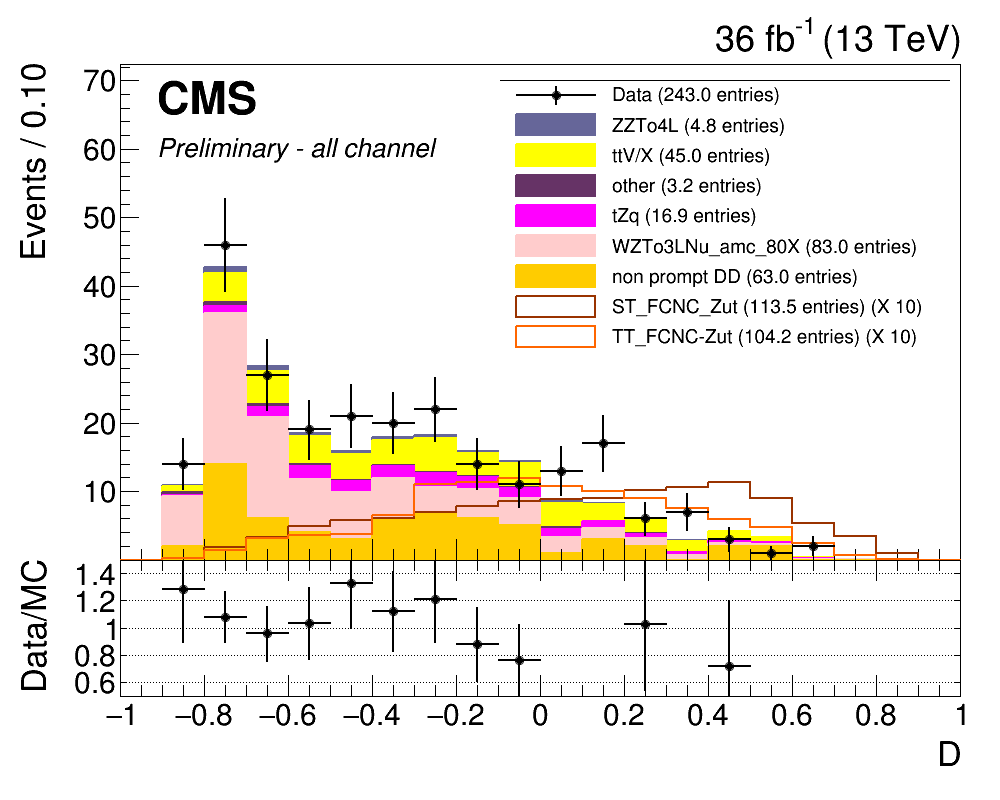
\includegraphics[width=0.47\linewidth]{FiguresAfterUnblinding/BDTunweighted//toppair_Zut_BDT_all_Stack}
	% % 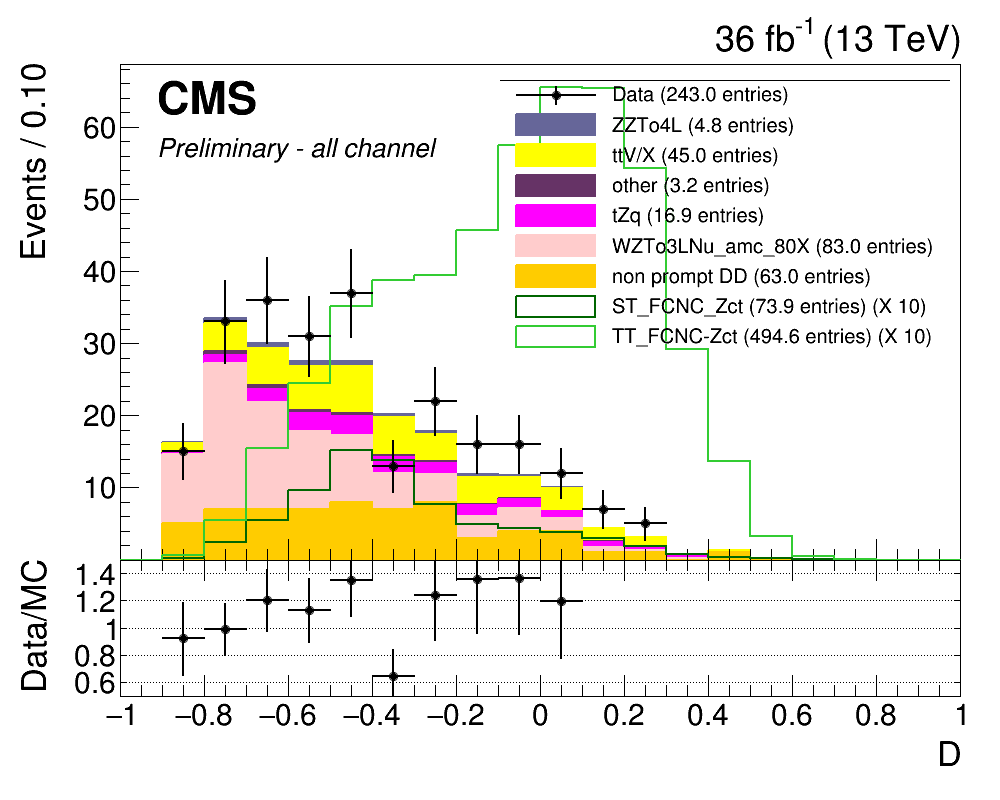
\includegraphics[width=0.47\linewidth]{FiguresAfterUnblinding/BDTunweighted//toppair_Zct_BDT_all_Stack}
	% % 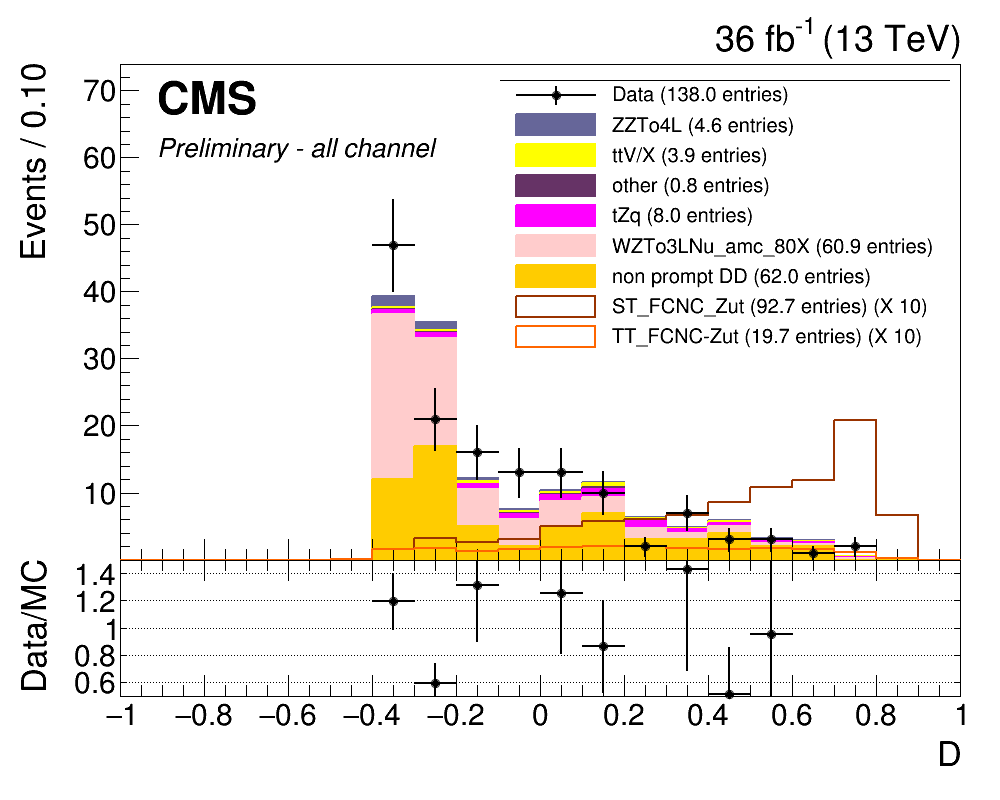
\includegraphics[width=0.47\linewidth]{FiguresAfterUnblinding/BDTunweighted//singletop_Zut_BDT_all_Stack}
	% % 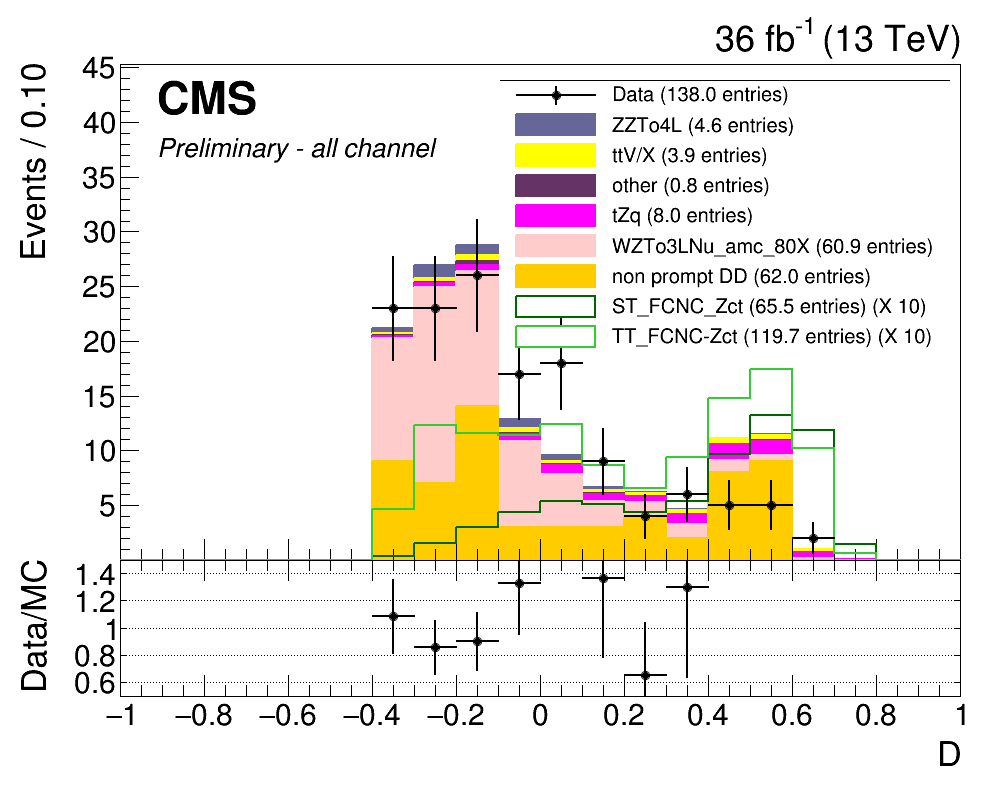
\includegraphics[width=0.47\linewidth]{FiguresAfterUnblinding/BDTunweighted//singletop_Zct_BDT_all_Stack}
	\caption{Distributions of the discriminating variable before the fit, all different leptonic channels together. Upper left: \TTSR\ \Zut , upper right: \TTSR\ \Zct ; lower left: \STSR\  \Zut , lower right: \STSR\  \Zct .}
	\label{fig:bdtallstack}
\end{figure}	

\begin{figure}[ht]
	\centering
	% % 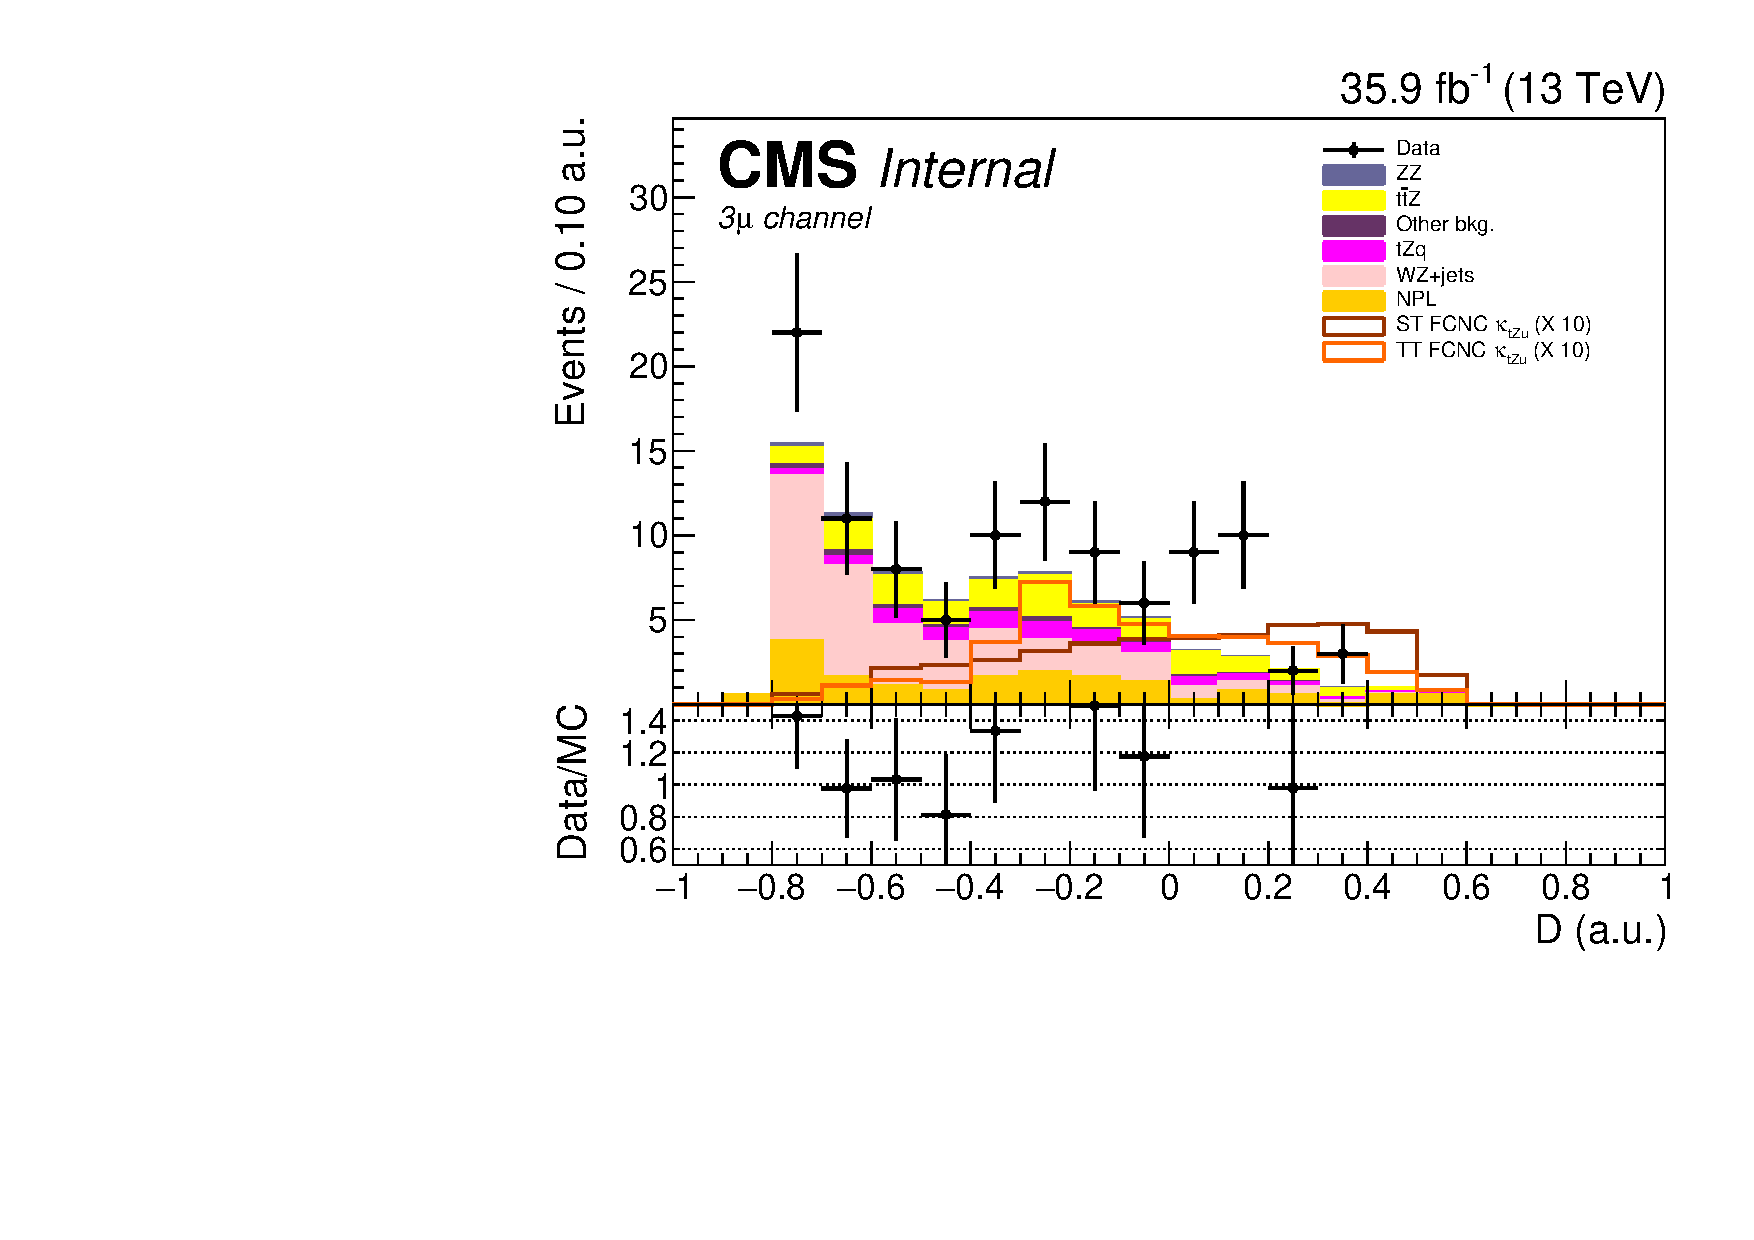
\includegraphics[width=0.47\linewidth]{FiguresAfterUnblinding/BDTunweighted//toppair_Zut_BDT_uuu_Stack}
	% % 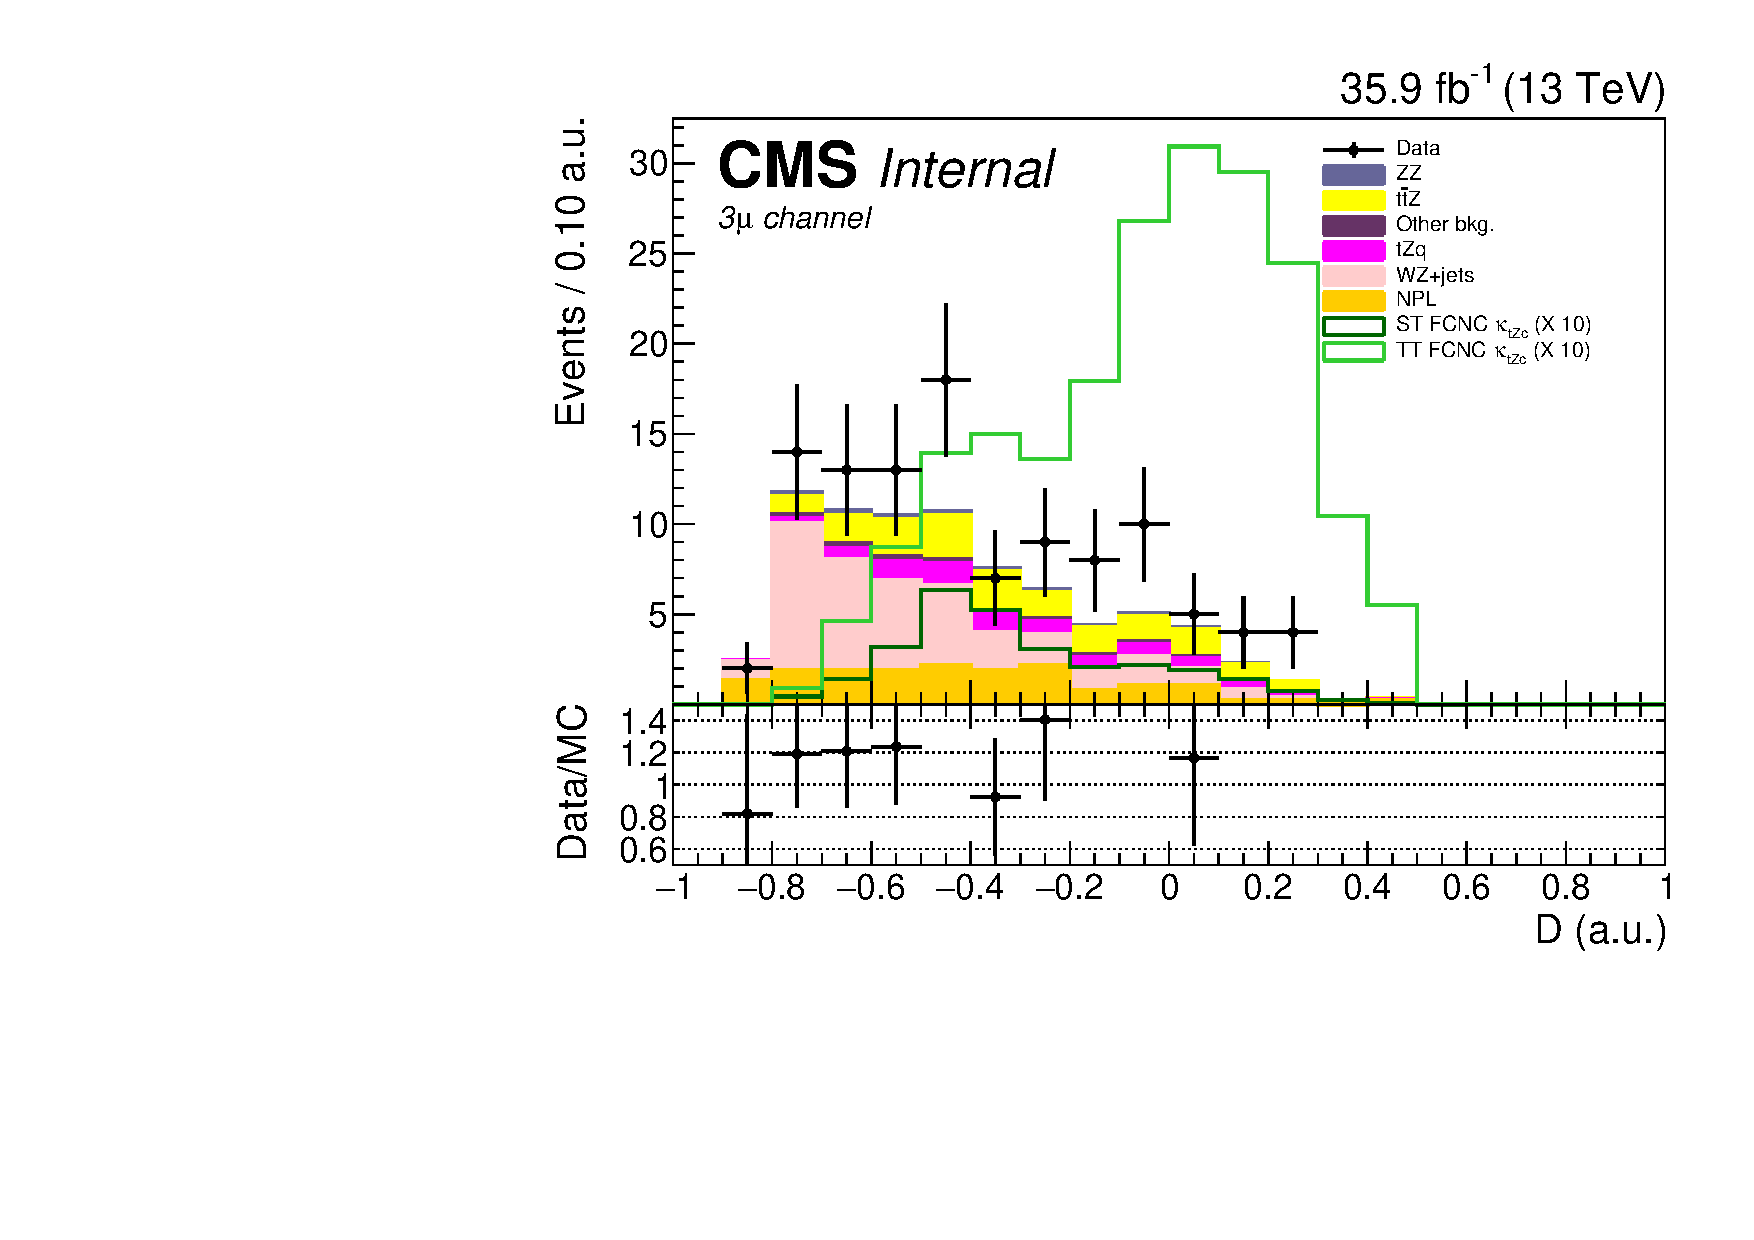
\includegraphics[width=0.47\linewidth]{FiguresAfterUnblinding/BDTunweighted//toppair_Zct_BDT_uuu_Stack}
	% % 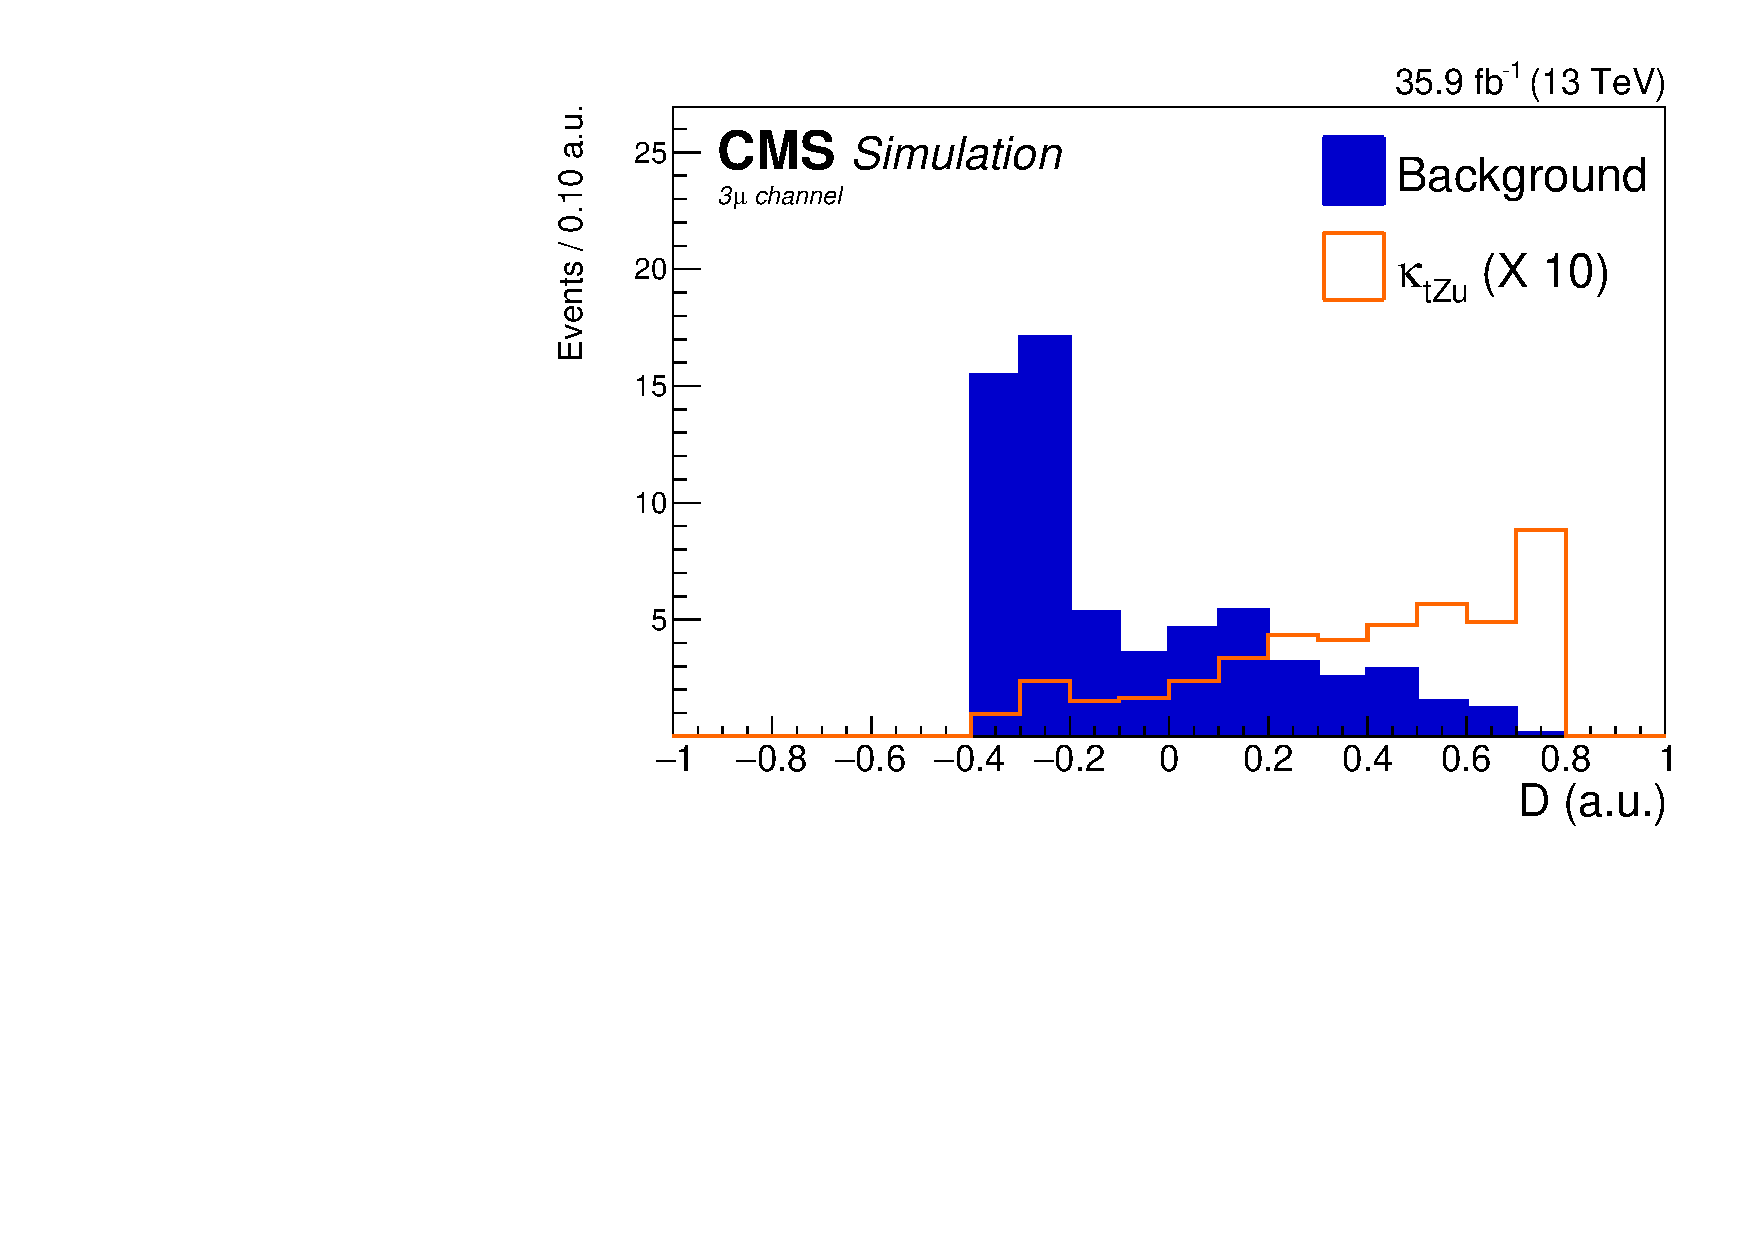
\includegraphics[width=0.47\linewidth]{FiguresAfterUnblinding/BDTunweighted//singletop_Zut_BDT_uuu_Stack}
	% % 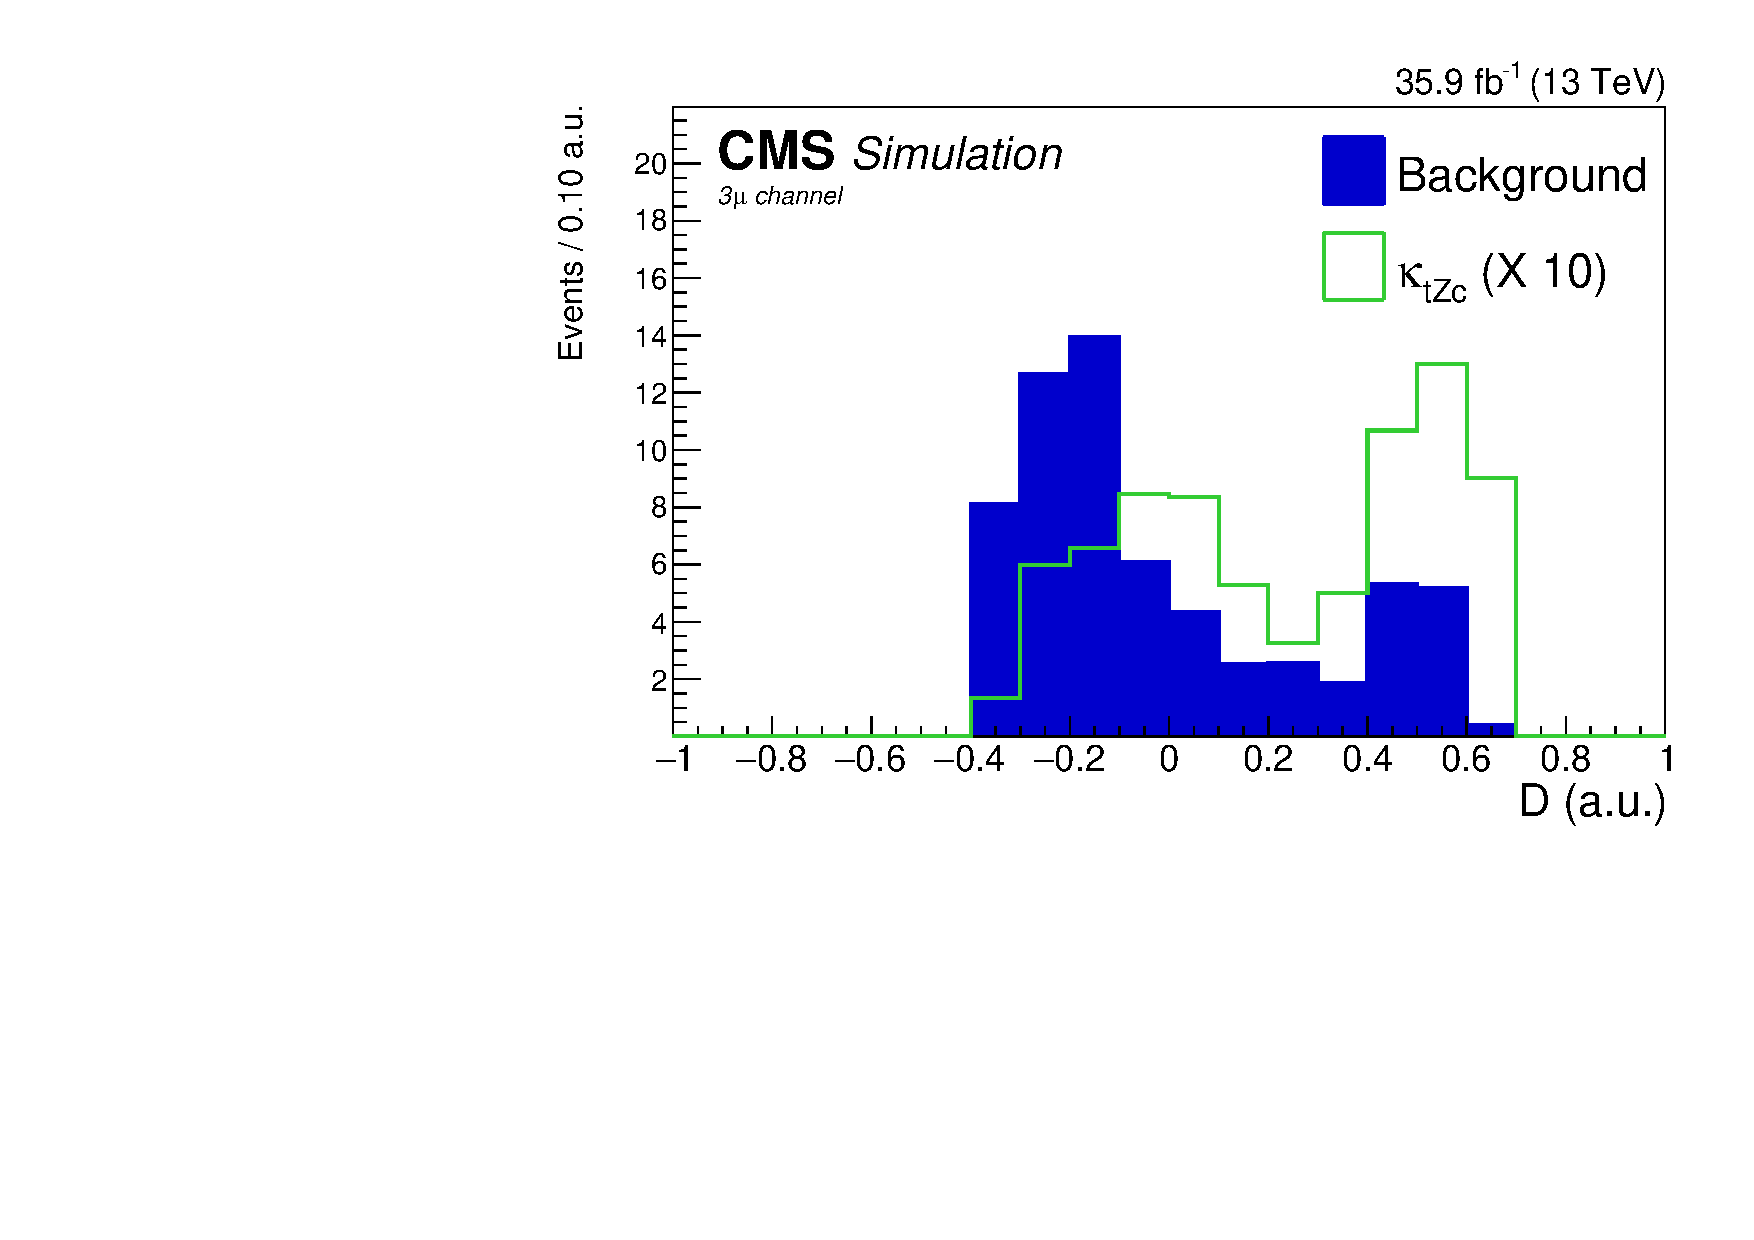
\includegraphics[width=0.47\linewidth]{FiguresAfterUnblinding/BDTunweighted//singletop_Zct_BDT_uuu_Stack}
	\caption{Distributions of the discriminating variable before the fit, \mumumu\  channel. Upper left: \TTSR\ \Zut , upper right: \TTSR\ \Zct ; lower left: \STSR\  \Zut , lower right: \STSR\  \Zct .}
	\label{fig:bdtuuustack}
\end{figure}


\begin{figure}[ht]
	\centering
	% % 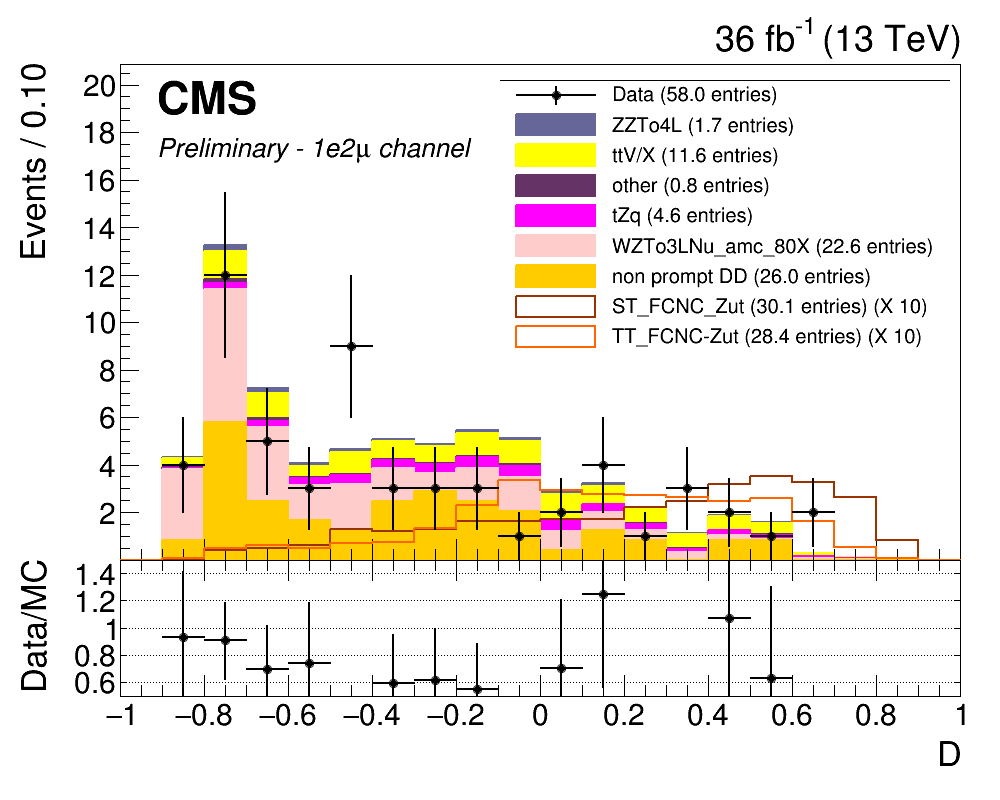
\includegraphics[width=0.47\linewidth]{FiguresAfterUnblinding/BDTunweighted//toppair_Zut_BDT_uue_Stack}
	% % 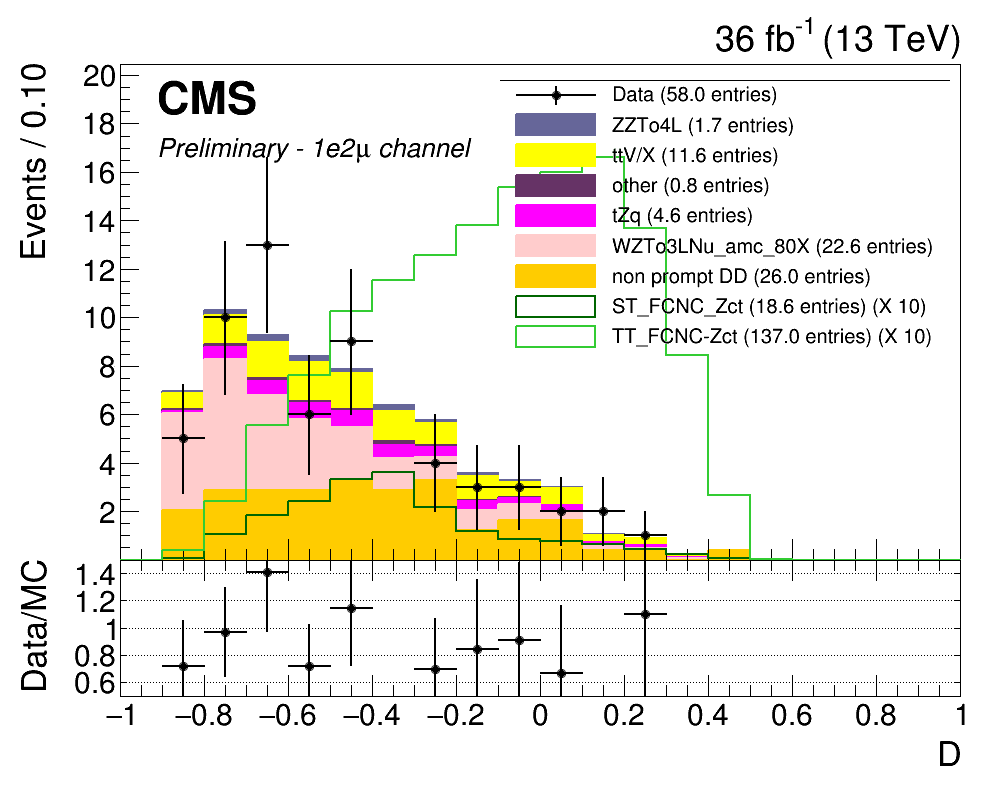
\includegraphics[width=0.47\linewidth]{FiguresAfterUnblinding/BDTunweighted//toppair_Zct_BDT_uue_Stack}
	% % 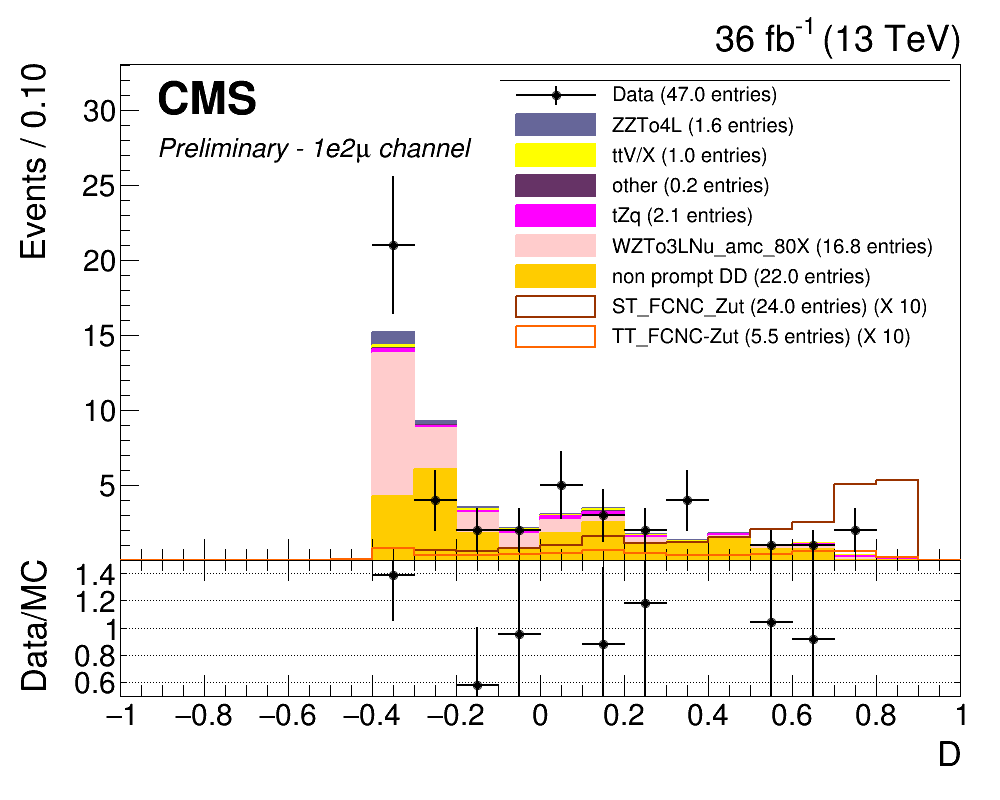
\includegraphics[width=0.47\linewidth]{FiguresAfterUnblinding/BDTunweighted//singletop_Zut_BDT_uue_Stack}
	% % 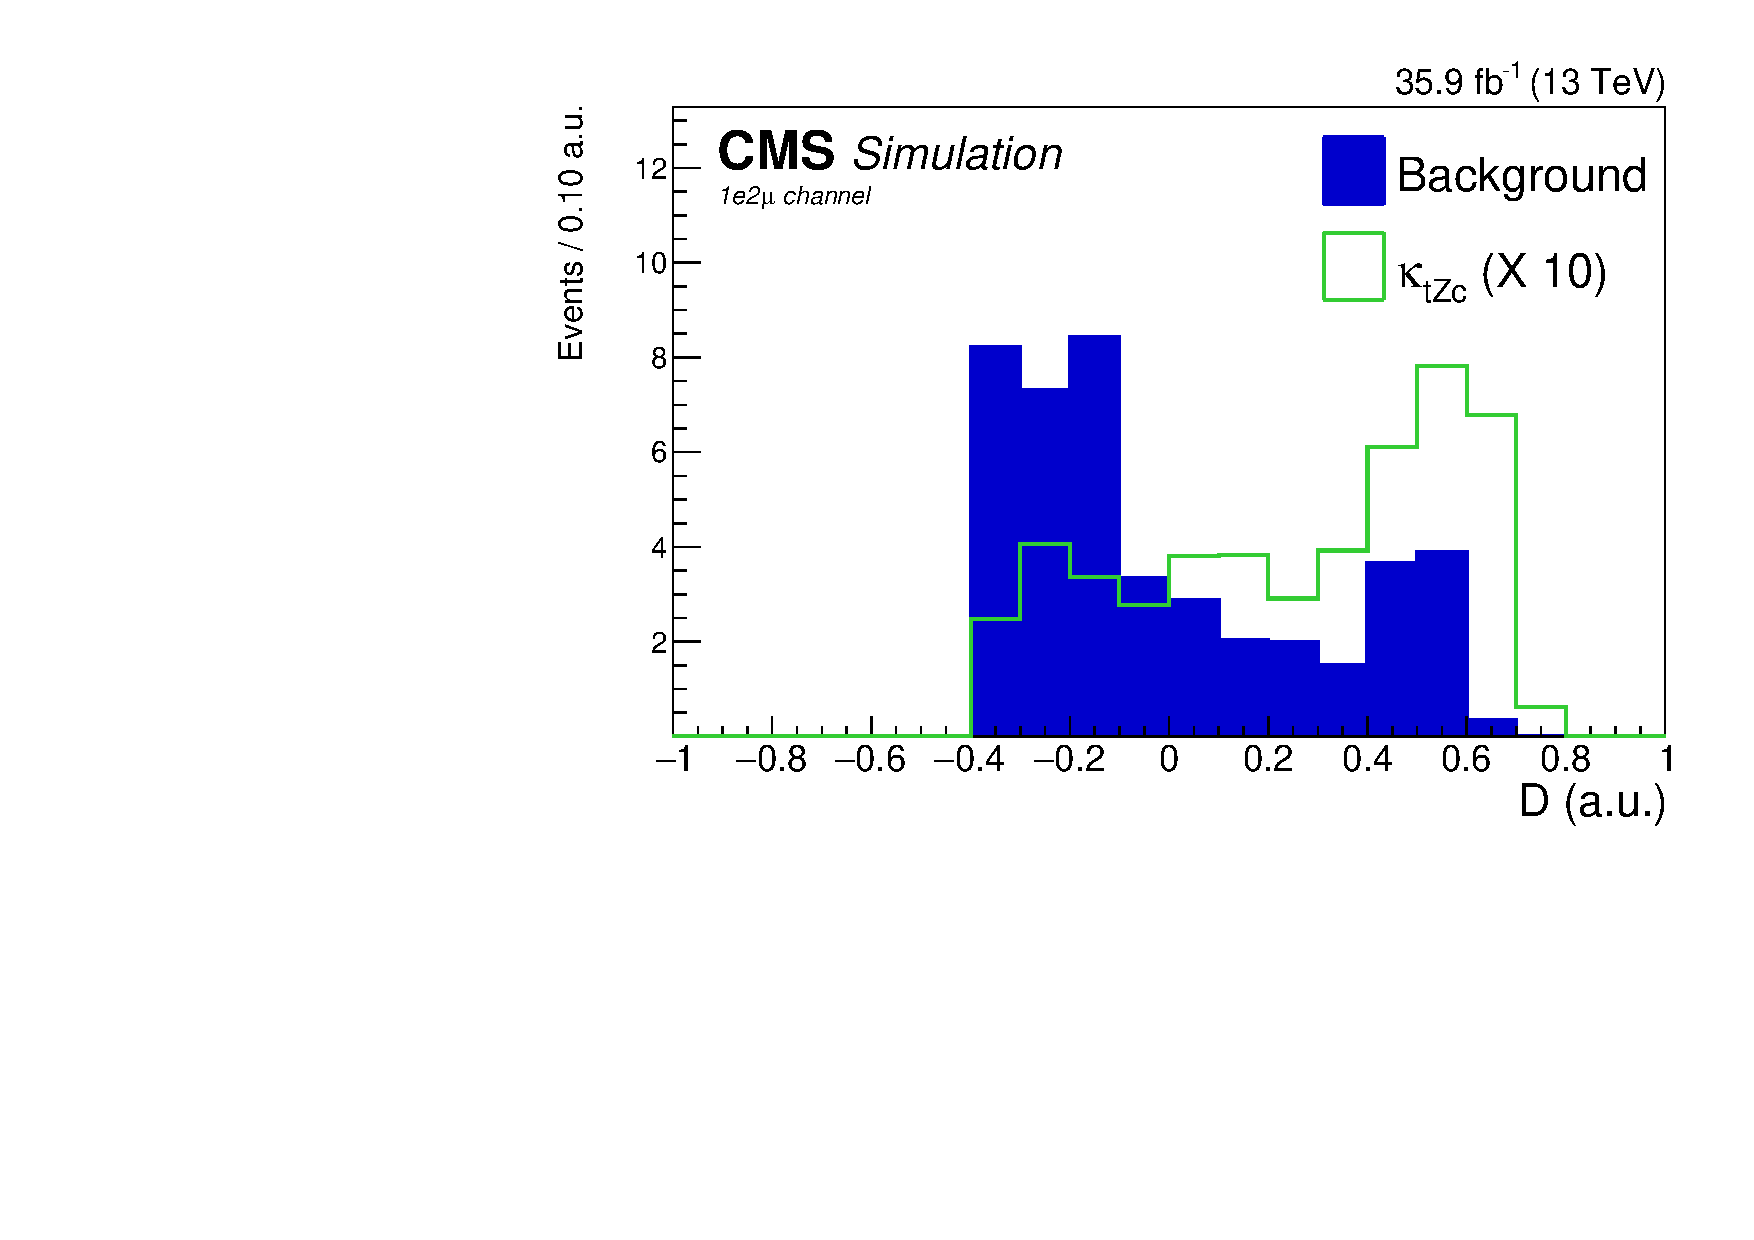
\includegraphics[width=0.47\linewidth]{FiguresAfterUnblinding/BDTunweighted//singletop_Zct_BDT_uue_Stack}
	\caption{Distributions of the discriminating variable before the fit, \emumu\  channel. Upper left: \TTSR\ \Zut , upper right: \TTSR\ \Zct ; lower left: \STSR\  \Zut , lower right: \STSR\  \Zct .}
	\label{fig:bdtuuestack}
\end{figure}

\begin{figure}[ht]
	\centering
	% % 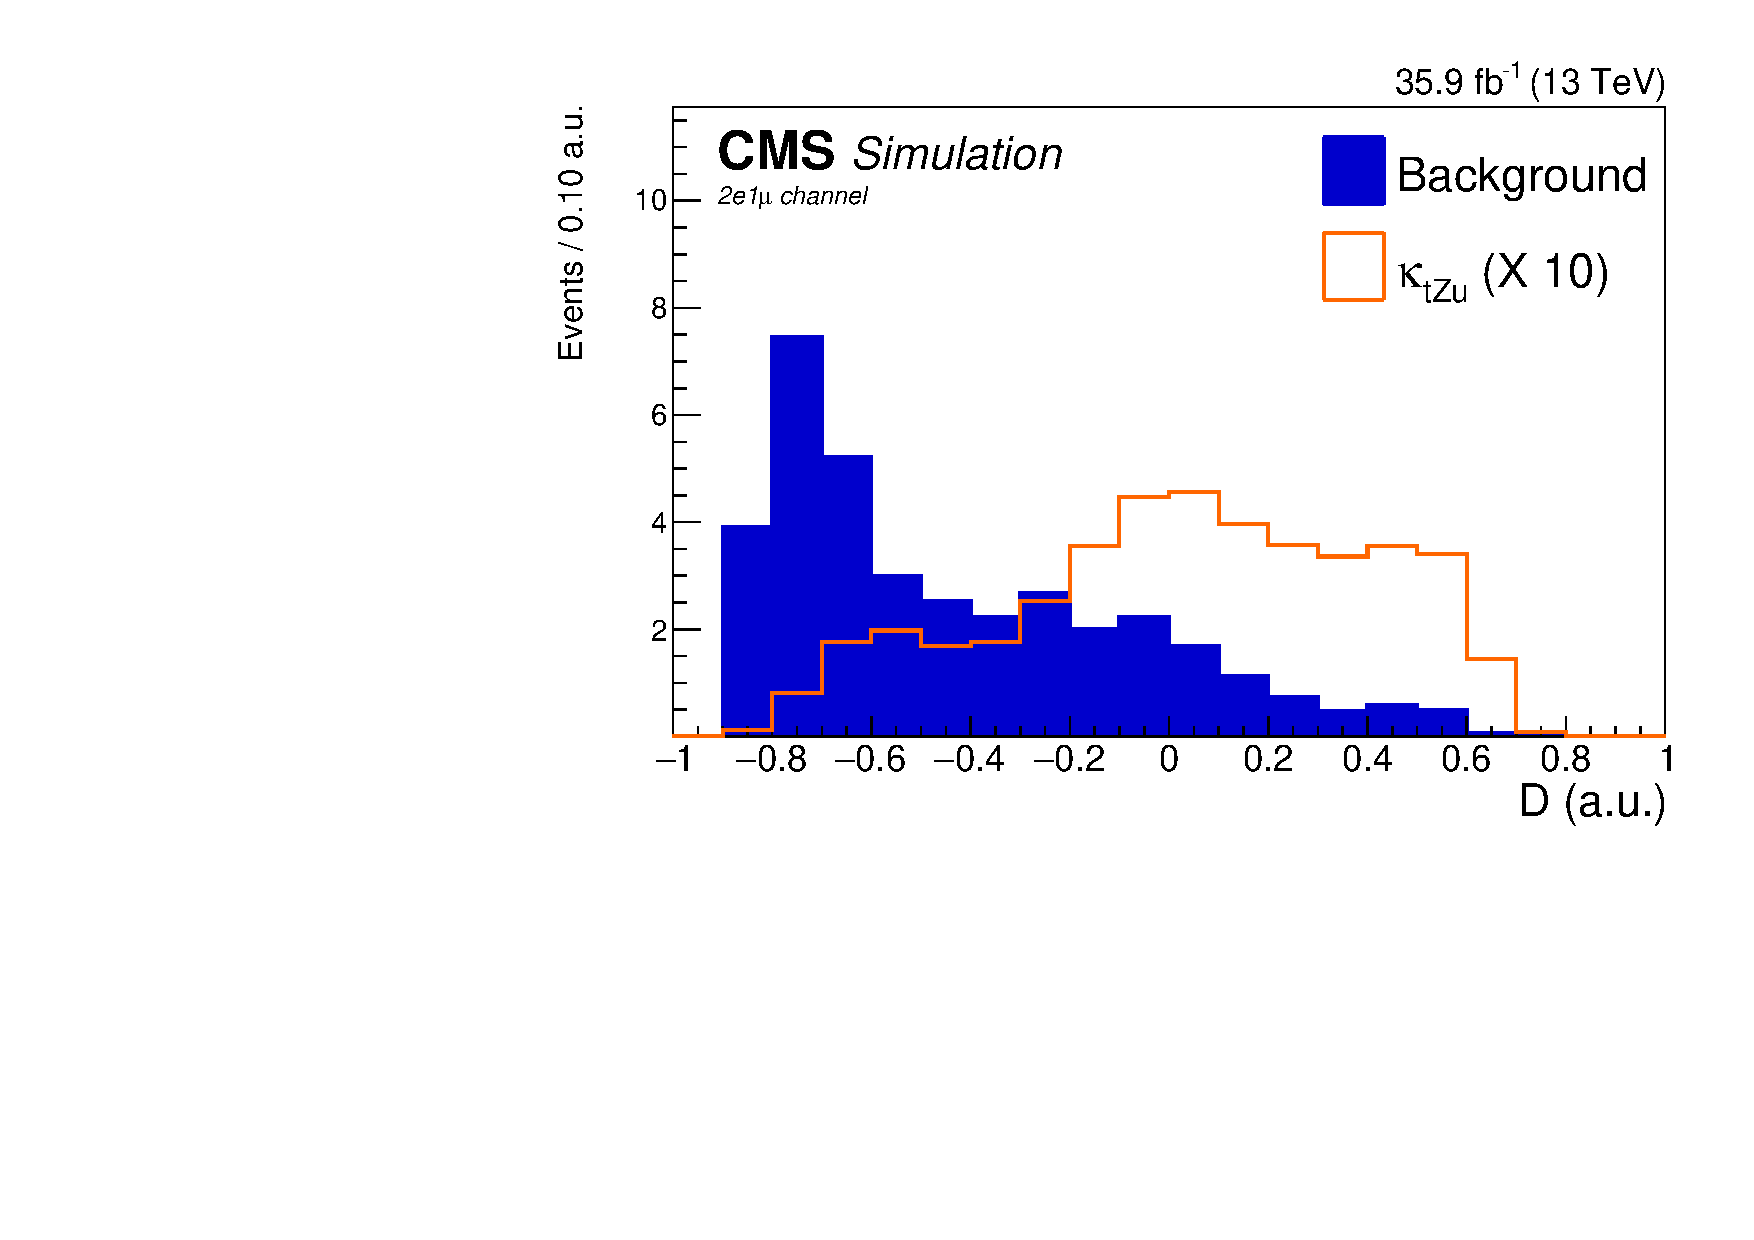
\includegraphics[width=0.47\linewidth]{FiguresAfterUnblinding/BDTunweighted//toppair_Zut_BDT_eeu_Stack}
	% % 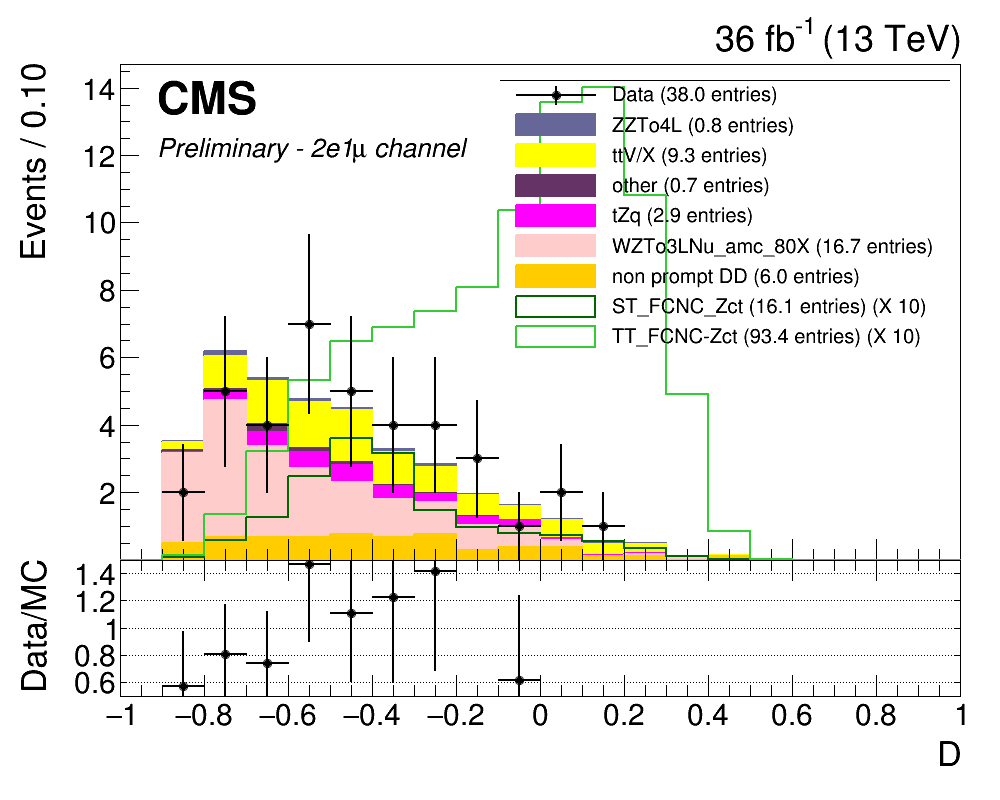
\includegraphics[width=0.47\linewidth]{FiguresAfterUnblinding/BDTunweighted//toppair_Zct_BDT_eeu_Stack}
	% % 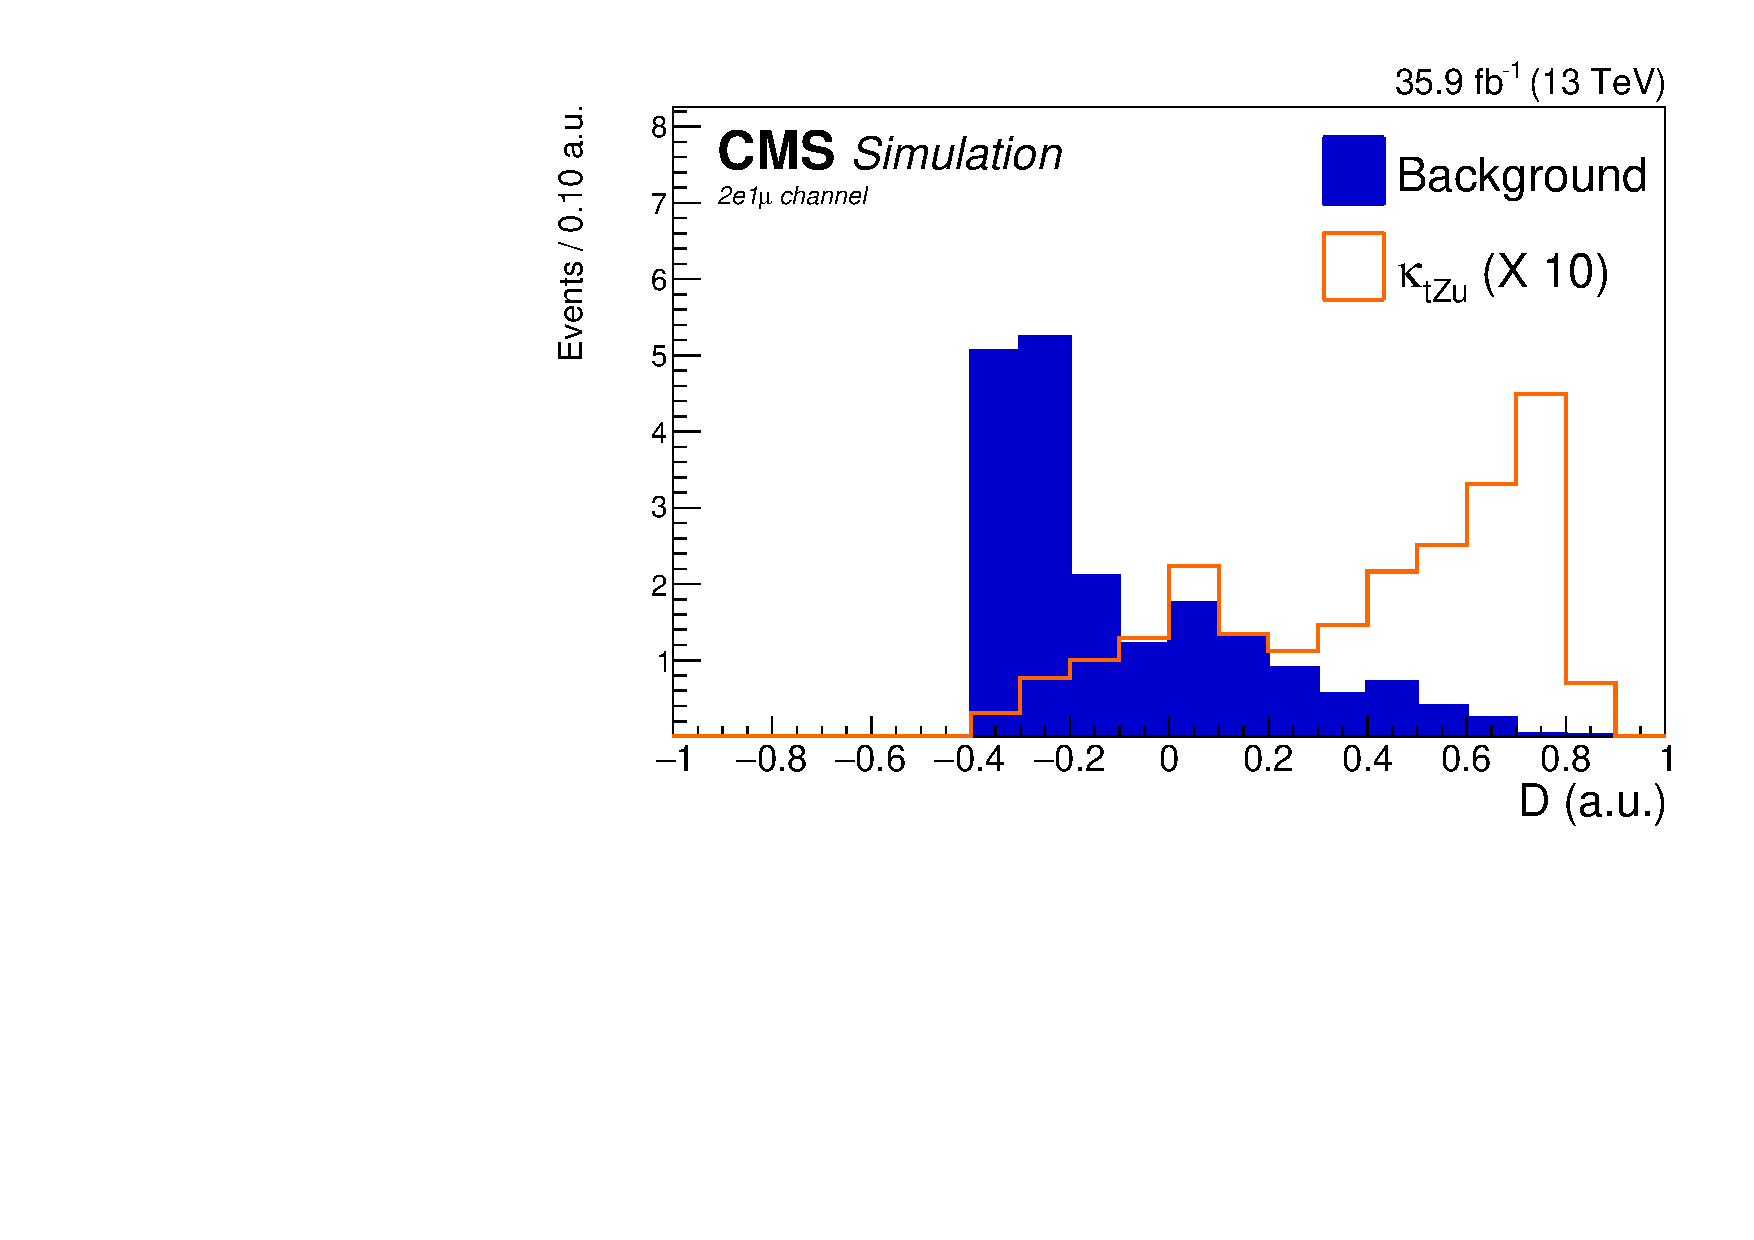
\includegraphics[width=0.47\linewidth]{FiguresAfterUnblinding/BDTunweighted//singletop_Zut_BDT_eeu_Stack}
	% % 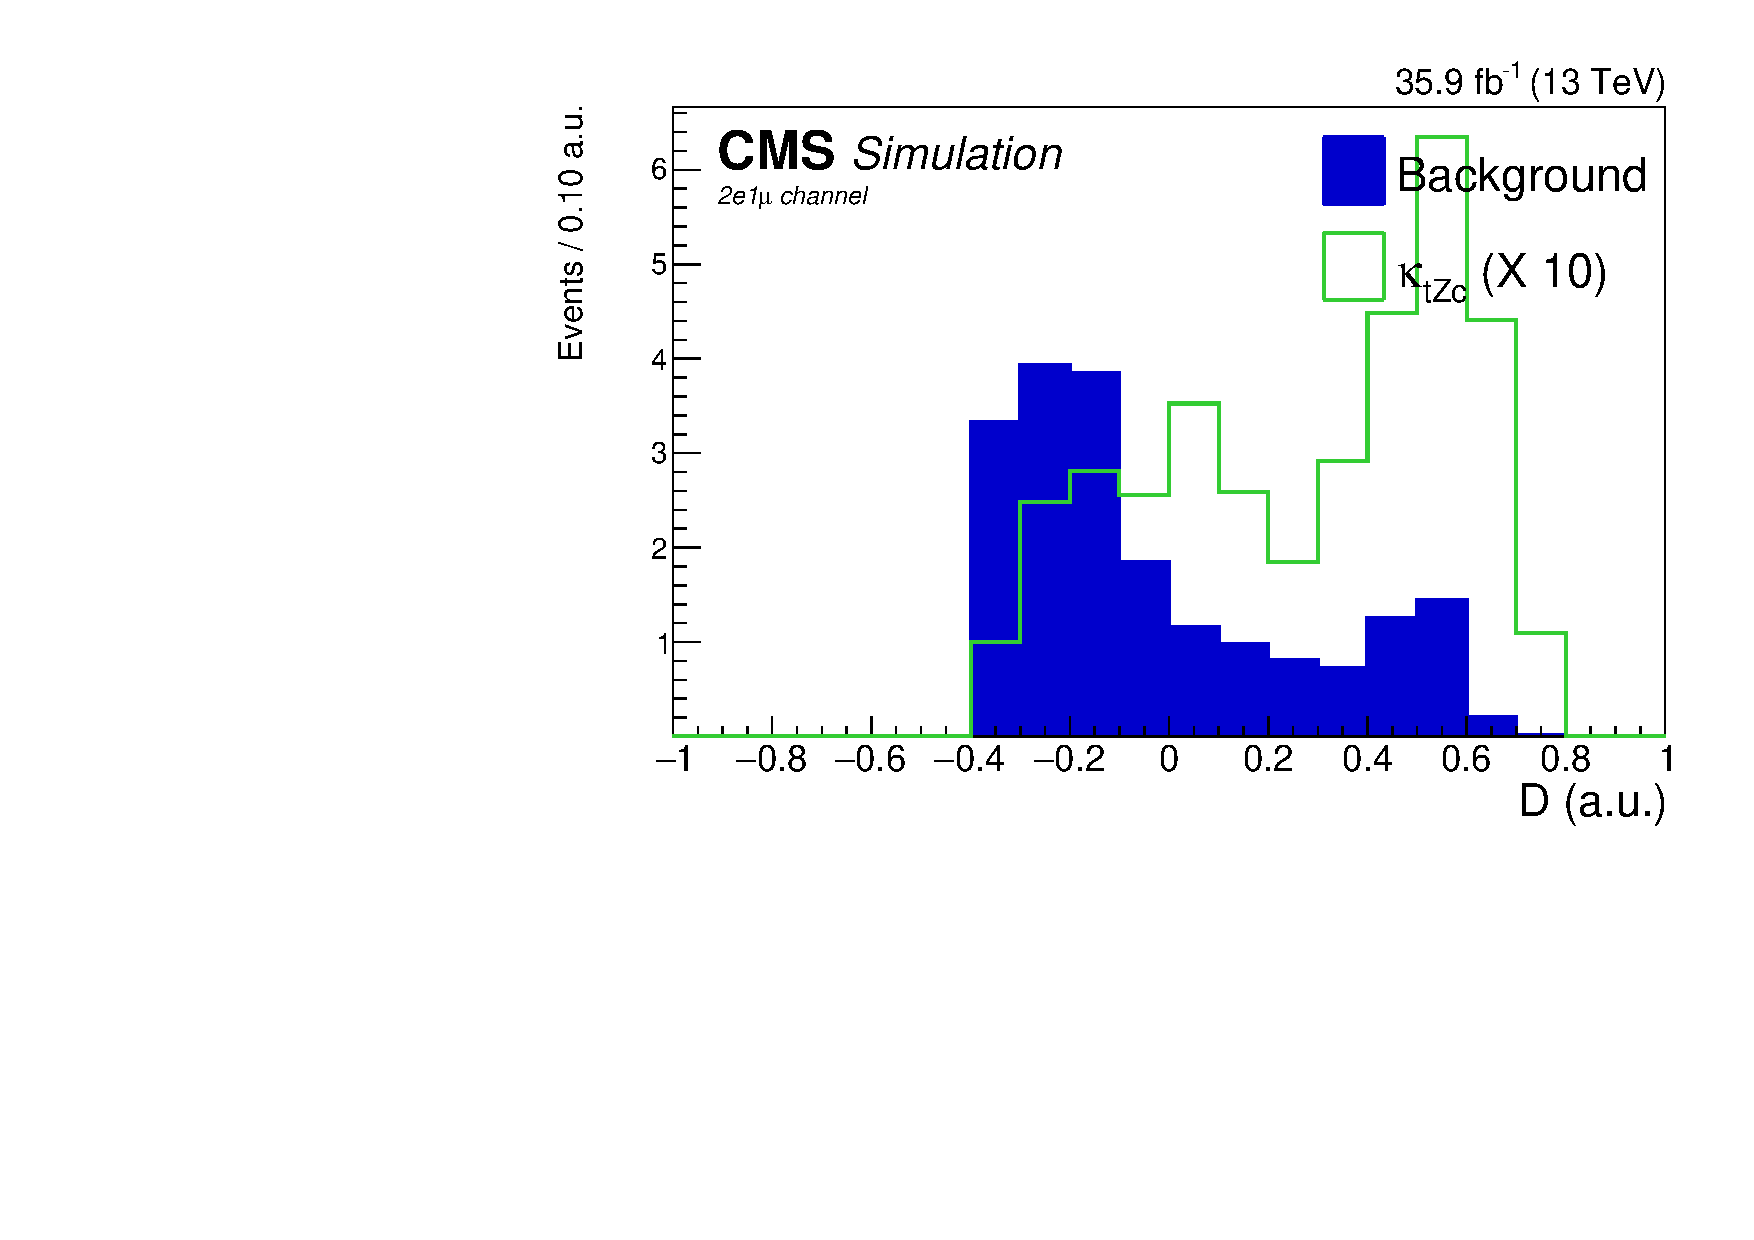
\includegraphics[width=0.47\linewidth]{FiguresAfterUnblinding/BDTunweighted//singletop_Zct_BDT_eeu_Stack}
	\caption{Distributions of the discriminating variable before the fit, \eemu\  channel. Upper left: \TTSR\ \Zut , upper right: \TTSR\ \Zct ; lower left: \STSR\  \Zut , lower right: \STSR\  \Zct .}
	\label{fig:bdteeustack}
\end{figure}



\begin{figure}[ht]
	\centering
	% % 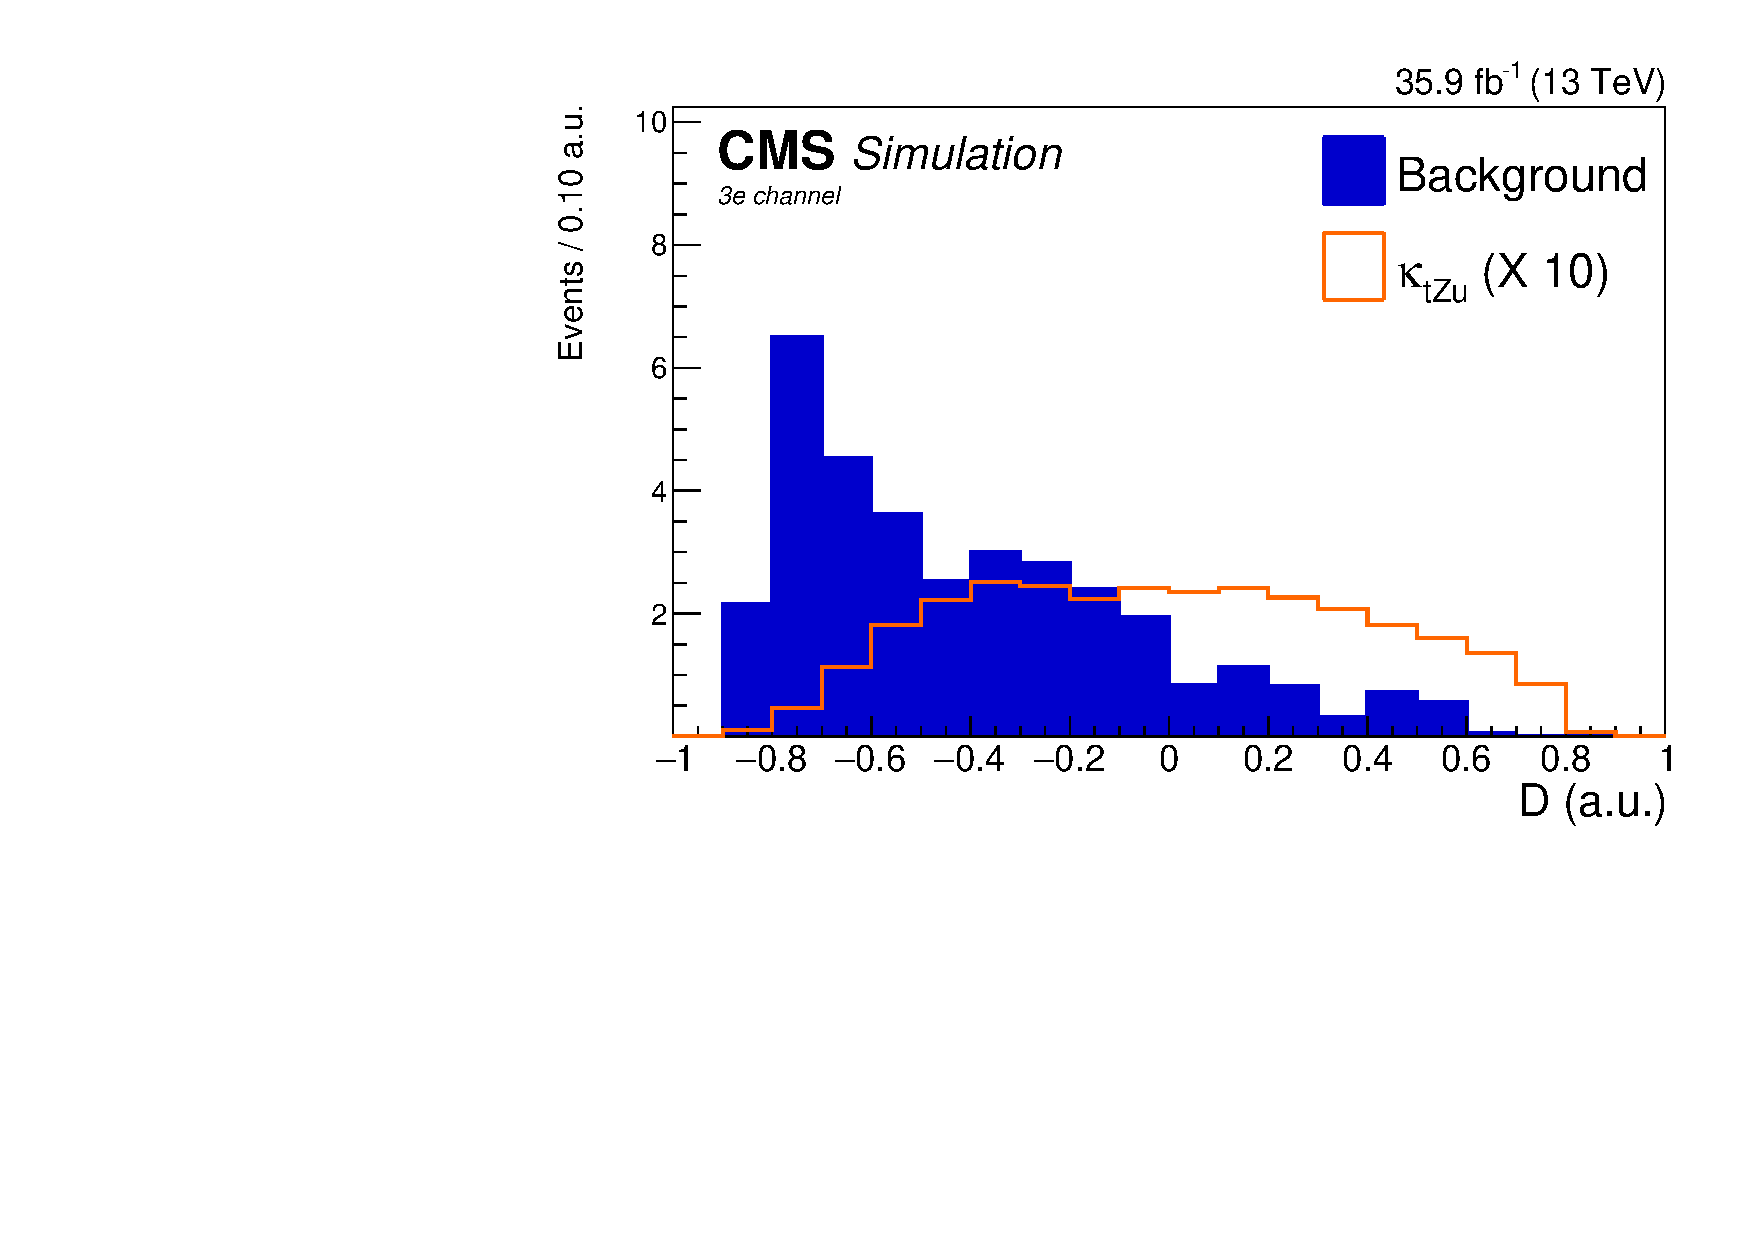
\includegraphics[width=0.47\linewidth]{FiguresAfterUnblinding/BDTunweighted//toppair_Zut_BDT_eee_Stack}
	% % 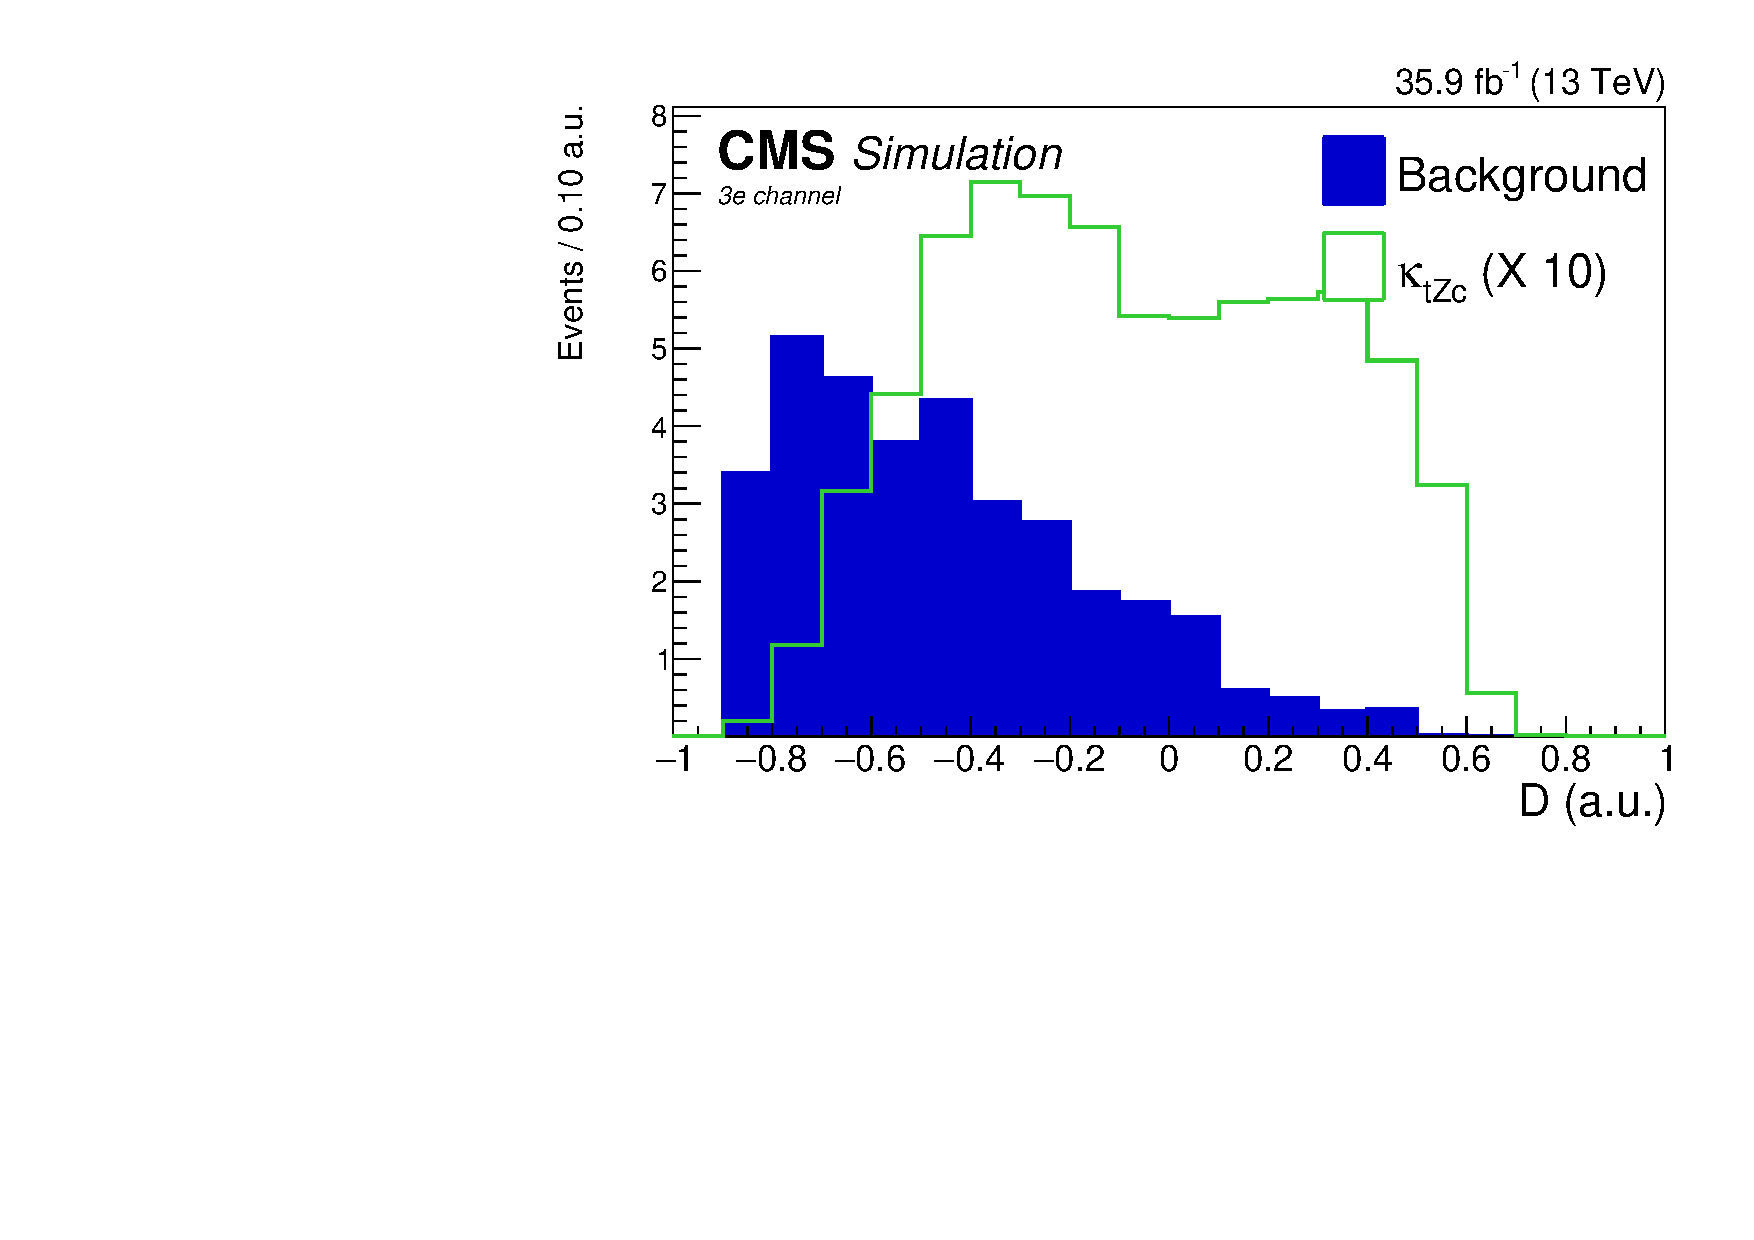
\includegraphics[width=0.47\linewidth]{FiguresAfterUnblinding/BDTunweighted//toppair_Zct_BDT_eee_Stack}
	% % 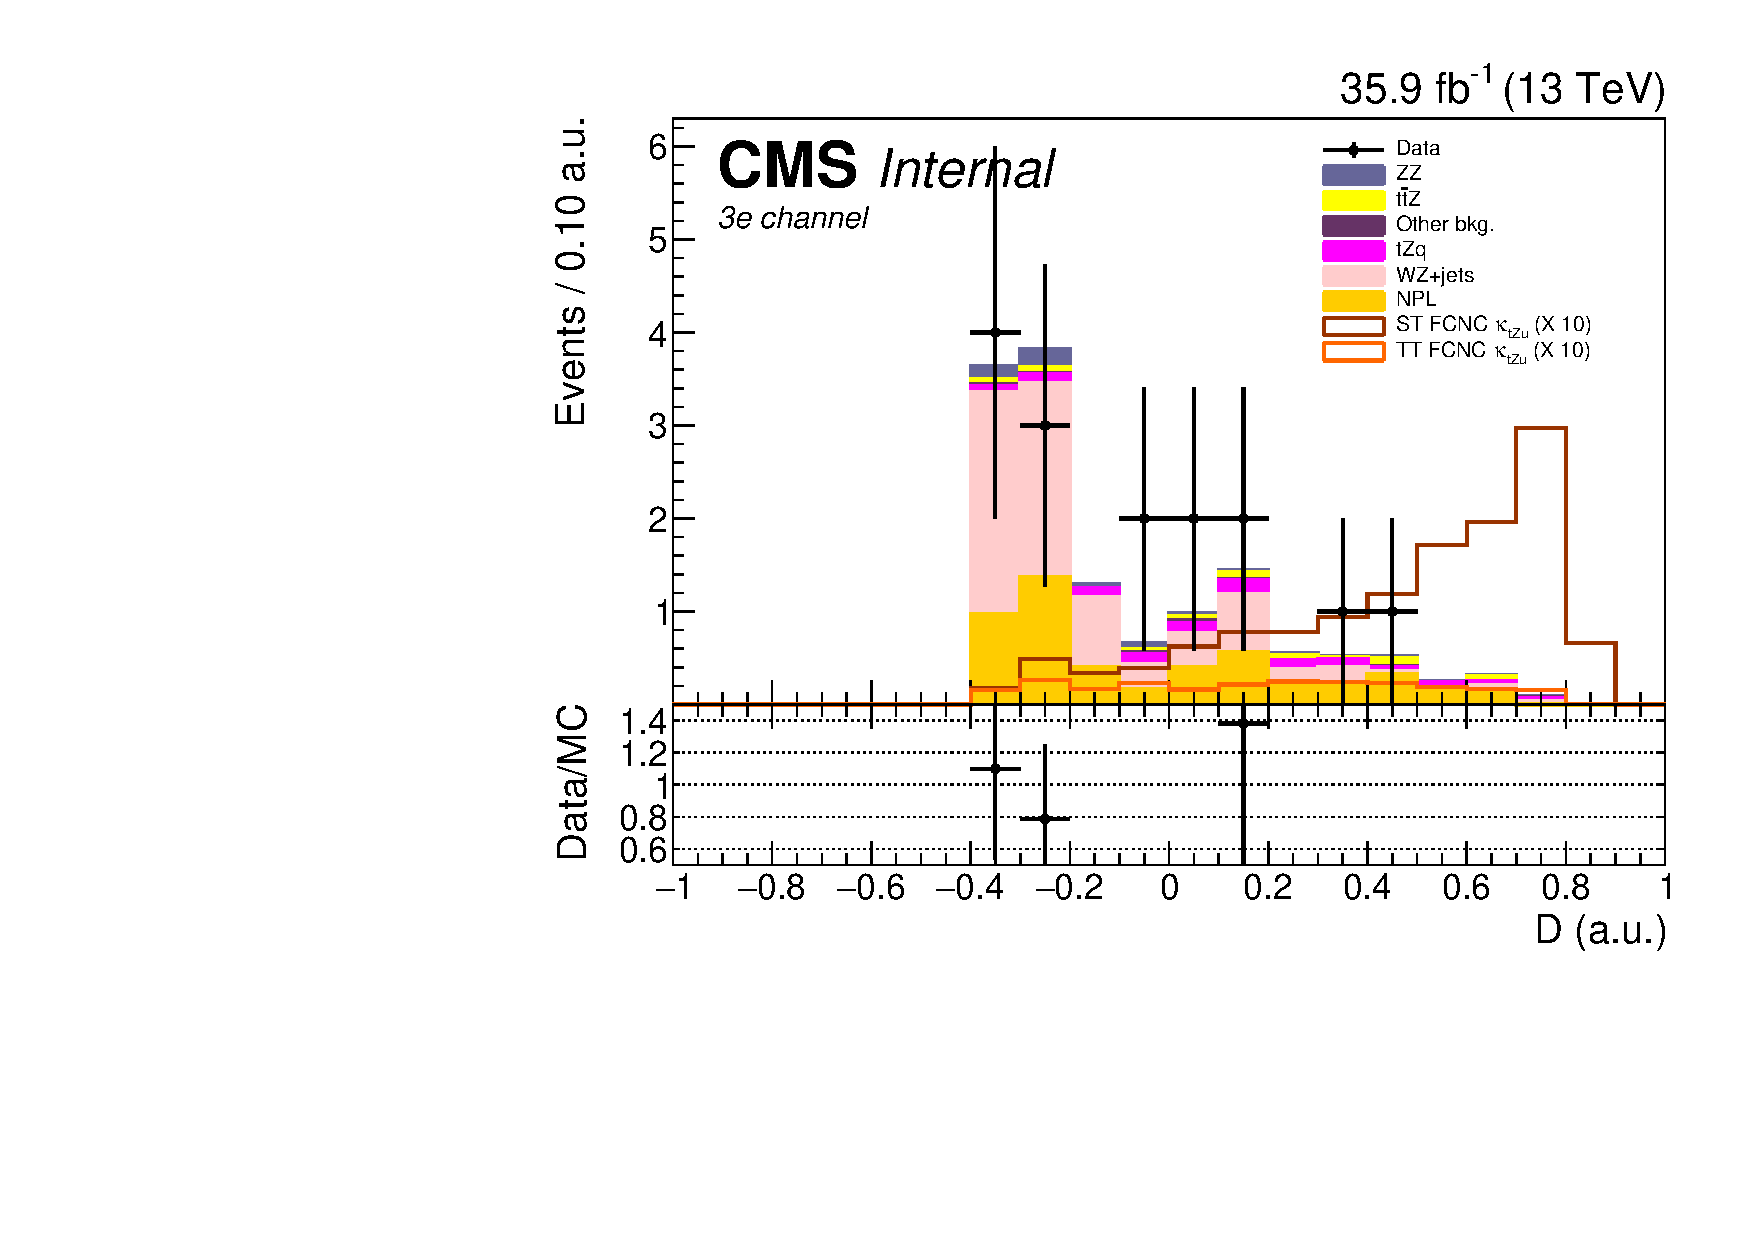
\includegraphics[width=0.47\linewidth]{FiguresAfterUnblinding/BDTunweighted//singletop_Zut_BDT_eee_Stack}
	% % 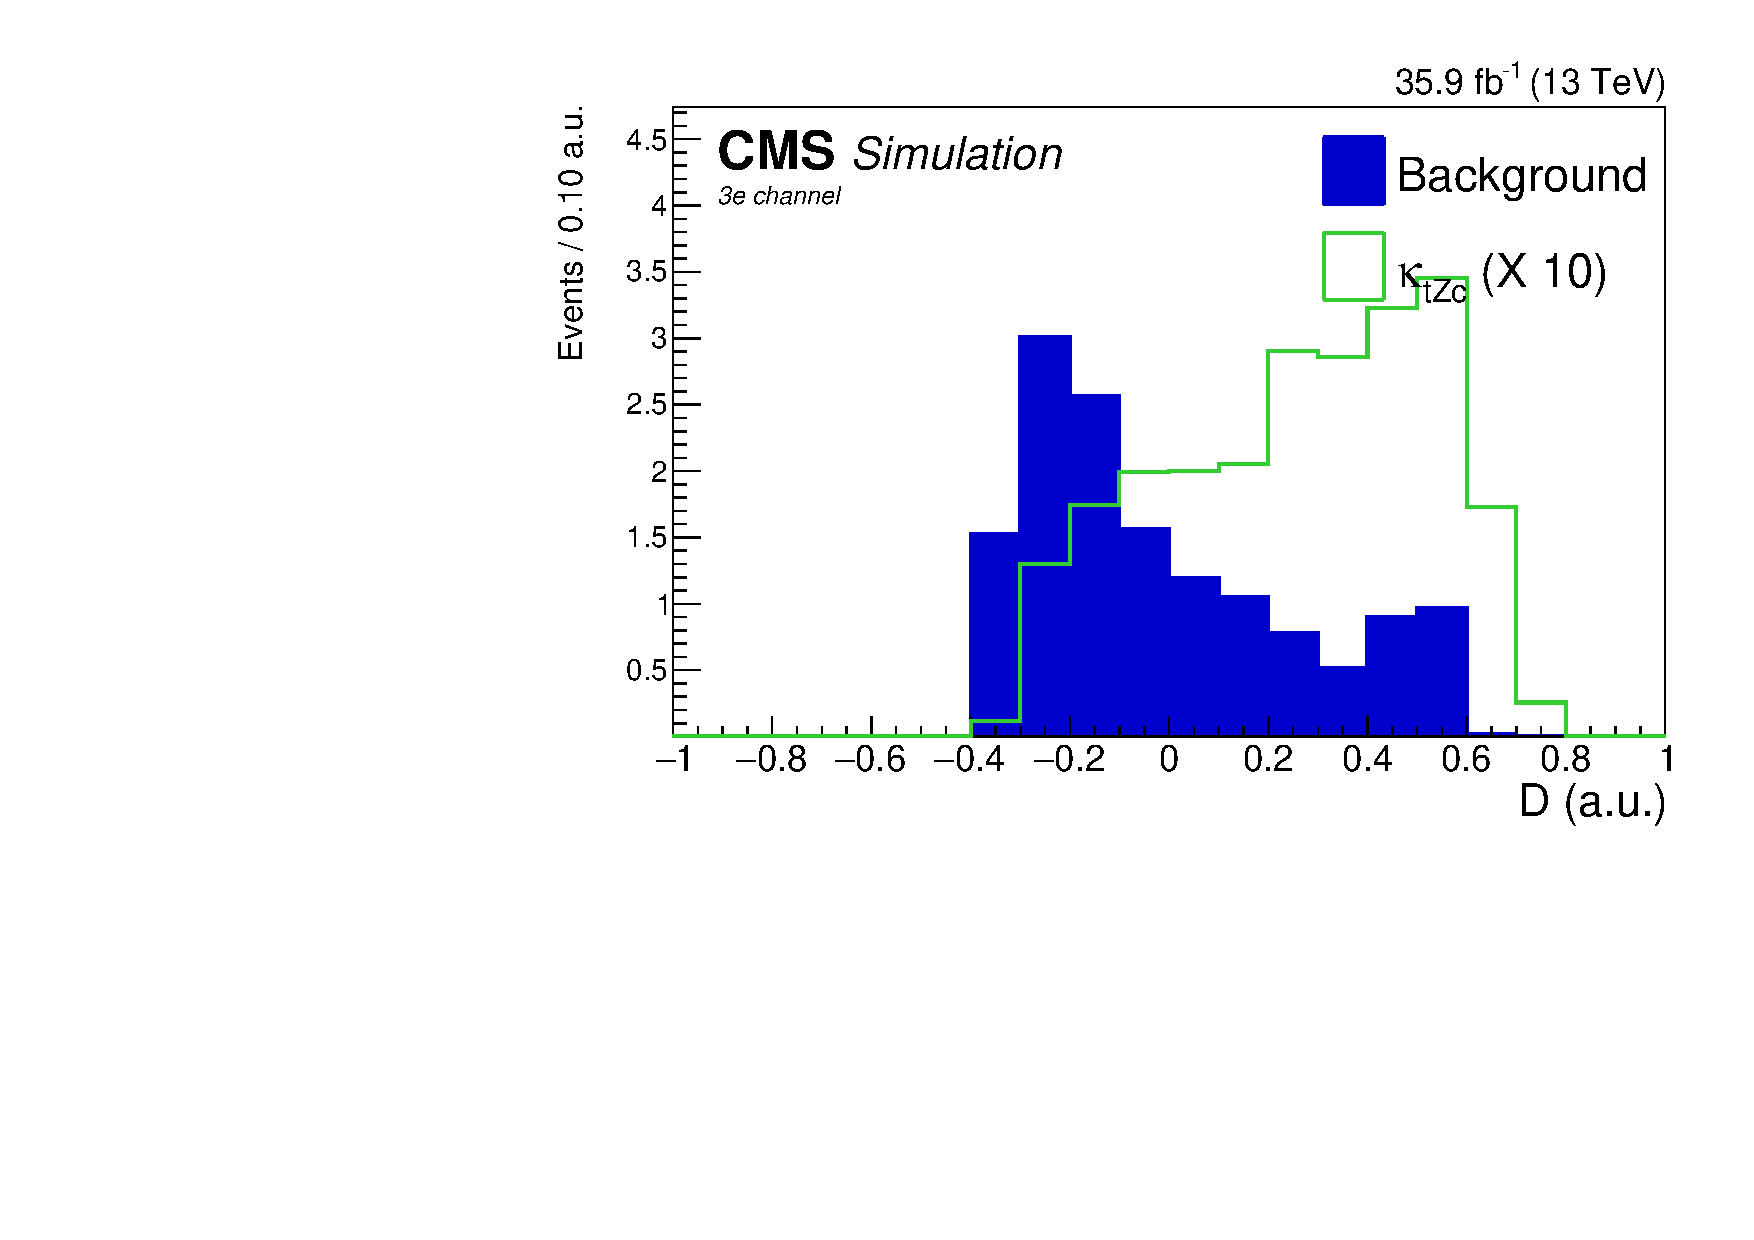
\includegraphics[width=0.47\linewidth]{FiguresAfterUnblinding/BDTunweighted//singletop_Zct_BDT_eee_Stack}
	\caption{Distributions of the discriminating variable before the fit, \eee\  channel. Upper left: \TTSR\ \Zut , upper right: \TTSR\ \Zct ; lower left: \STSR\  \Zut , lower right: \STSR\  \Zct .}
	\label{fig:bdteeestack}
\end{figure}

\subsection{Transverse mass in \WZCR}
The \WZCR\ is used to estimate the contribution from \WZ+jets and \NPL\ background. In this region, a fit is performed on the transverse mass distribution of the \PW\ boson. The pre-fit templates are given in \fig{fig:mtwallstack}. 

\begin{figure}[ht]
	\centering
	% % 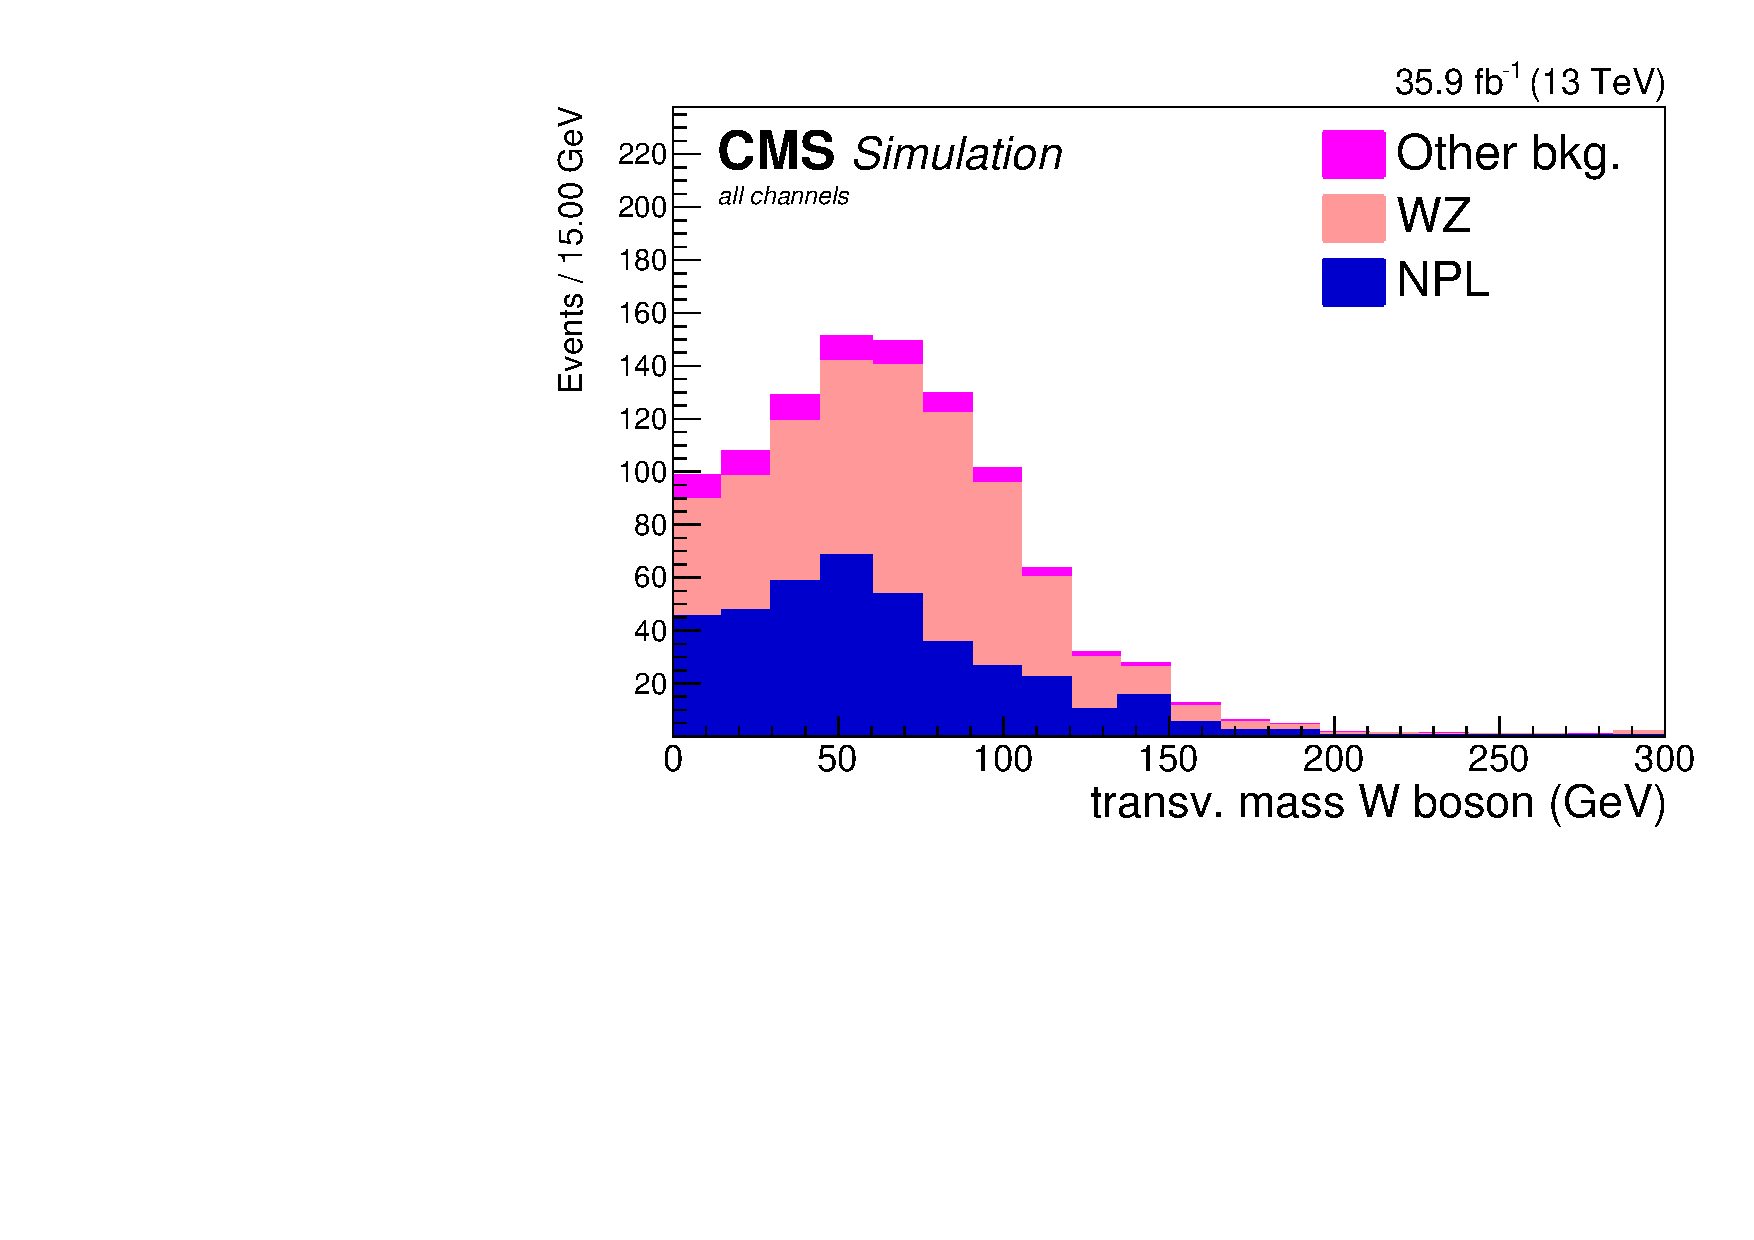
\includegraphics[width=0.47\linewidth]{FiguresAfterUnblinding/MSPlotMTW/MTW_all_Stack}
	% % 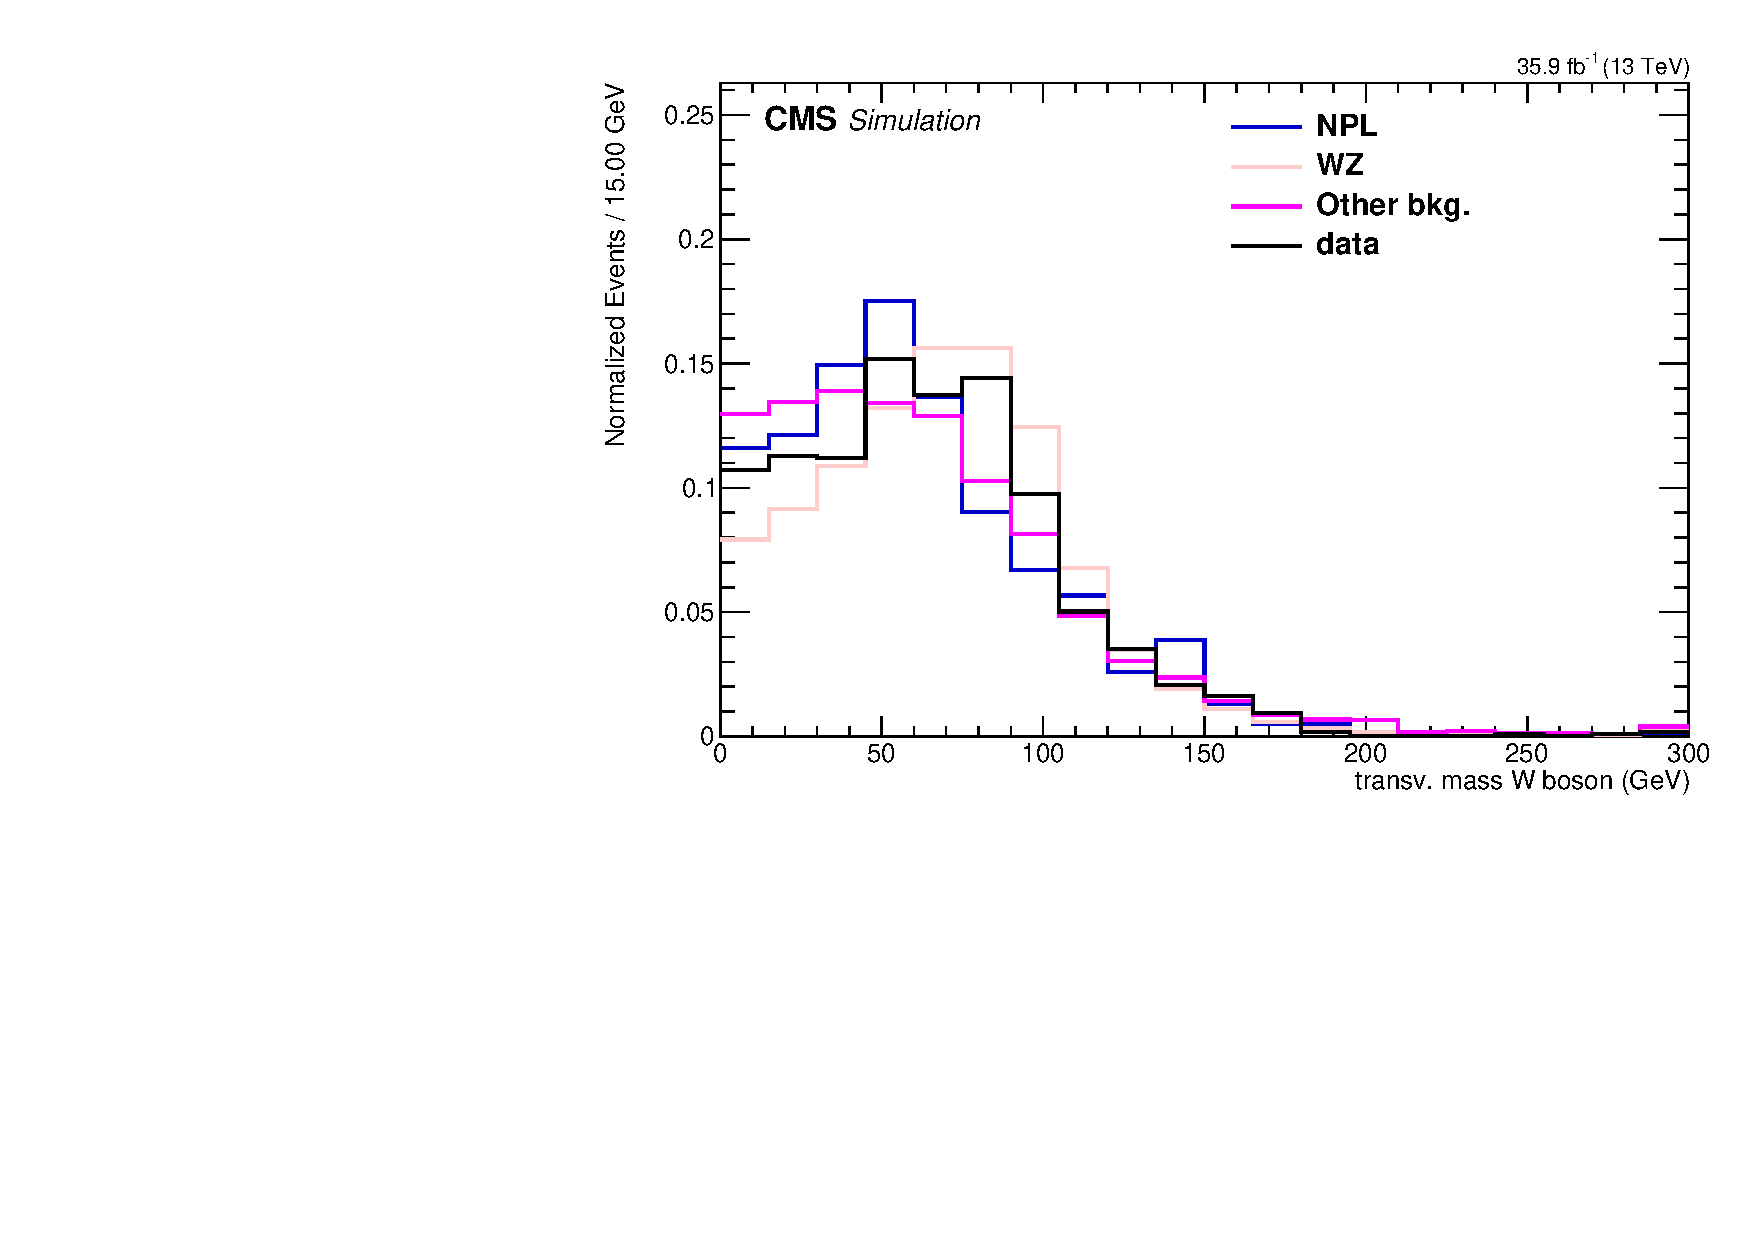
\includegraphics[width=0.37\linewidth]{FiguresAfterUnblinding/MSPlotMTW/MTW_all_Normalized}
	\caption{The transverse mass of the W boson in the \WZCR, before the fit. All different leptonic channels together. Left: scaled to the data, right: normalized.}
	\label{fig:mtwallstack}
\end{figure}

\section{Systematic uncertainties}
The systematic uncertainties entering the analysis are coming from different sources. The experimental uncertainties arise from the reconstruction of the objects and are discussed in \Sec{{sec:PhysicsObject}}. These influence the number of events passing the selection, so-called normalisation uncertainties, or the relative occupancies of the distributions, so-called shape
 uncertainties. The normalisation uncertainties coming from reconstruction include the uncertainty of 2.5\% on the measured integrated luminosity and the efficiency of the trigger logic used for the analysis which has a 1\% (5\%) uncertainty on the 
 \mumumu\ and \emumu (\eemu\ and \eee) channels. The  pileup distribution is calculated via the minimum bias cross section which has a 4.6\% uncertainty. This uncertainty results in a systematic shift in the pileup distribution and its shape effect is estimated by recalculating the pileup distribution for each variation of the minimum bias cross section. The effect of the systematic upwards and downwards shift on the pileup distribution is demonstrated in \Sec{pileupsys}. The shape uncertainties also include the uncertainties coming from the applied lepton scale factors. Their systematic uncertainty originates from three sources: identification, isolation and tracking. The effect of systematic upwards or downwards shift on shapes is demonstrated
 in \Sec{sec:electronsys} and \Sec{sec:muonsys}. The uncertainties arising from jet energy corrections require a recalculation of all jet related kinematic observables and its effect is propagated to the missing transverse energy. The resulting effect of the systematic upwards or downwards shift on shapes is demonstrated in \Sec{sec:JESsys} and \Sec{sec:JERsys}. The reweighting of the CSVv2 discriminant is also a source of uncertainty. There are three sources of uncertainty contributing to the measurement of the b-tag related scale factors: statistical uncertainties, jet energy scale and the purity of the sample. These result in eight uncorrelated contributions for which the effects on the shapes are shown in \Sec{sec:btagsys}. 
 
 Since the \NPL\ sample is artificially made from data by inverting the isolation of the third lepton. Its effect has to be estimated. The shape uncertainty one the \NPL\ processes is obtained by varying the isolation inversion with respect to tight working point to the loose working point for electrons and muons at the same time. This found to have negligible effect. The uncertainty on the normalisation of the overall \NPL\ yield is taken as 50\% in accordance the the \SM\ \tZq\ search\todocite.
 
 The uncertainty on the expected yield of the simulated backgrounds is taken to be 30\% of the yield such that it covers all uncertainties at next to leading order accuracy. Theory uncertainties  originating from the modelling of the main backgrounds are estimated to account for the effect on the shape of the distributions from the choice of parton density funnctions, and renormalization (\muR) and factorization (\muF) scales. The effect of the  renormalization (\muR) and factorization (\muF) scales is estimated by varying each independently and correlated up and down by a factor of two, where the anti-correlated variations are dropped. The envelope of these variations is used as an uncertainty. The uncertainties coming from the parton density functions  used for simulation are estimated using the PDF4LHC recipe~\cite{Ball:2017nwa}, which combines the MMHT14, CT14, and NNPDF3.0 PDF sets~\cite{Ball:2017nwa}. The theory uncertainties are considered for the main backgrounds coming from simulation: \WZ+jets, \ZZ+jets, \ttZ, and \tZq. This is found to have a negligible effect.

 The way the uncertainties are treated as nuisance parameters is summarized in Table \ref{tab:nuis}.

\begin{table}[htbp]
	\centering
	\caption{Uncertainties used in this analysis. The column labelled type represents how the uncertainty is treated for the fit.}
	\begin{tabular}{ccc}
		\toprule
		Source & Systematic input & Type \\ 
		\midrule 
		nonprompt muon norm. & 50\% & normalisation \\ 
		 
		nonprompt electron norm. & 50\% & normalisation \\ 
		 
		background \ttZ\ norm & 30\% & normalisation \\ 
		 
		background \WZ\ norm & 30\% & normalisation \\ 
		 
		background \tZq\ norm & 30\% & normalisation \\ 
		 
		background \ZZ\ norm & 30\% & normalisation \\ 
		 
		background other MC norm & 30\% & normalisation \\ 
		 
		trigger & 1\% (5\%) & normalisation \\ 
		 
		lepton identification  & $\pm \sigma(p_{T},\eta)$ & shape \\ 
		 
		JES & $\pm \sigma(p_{T},\eta)$ & shape \\ 
		 
		JER & $\pm \sigma(p_{T},\eta)$ &  shape \\ 
		 
		b-tagging & $\pm \sigma(p_{T},\eta)$ & shape \\ 
		 
		pileup\ & $\pm \sigma$ of min. bias cross section &  shape \\ 
		 
		PDF & PDF4LHC recipe &  shape (WZ,tZq, ttZ, ZZ)  \\ 
		 
		luminosity & 2.5\% & normalisation \\ 
		 
		renorm. and fact. scales & varying indep. and corr. &  shape \\ 
		\bottomrule
	\end{tabular} 
	\label{tab:nuis}
\end{table}
\begin{comment}
\subsection{Effect of pile up on the shapes}
\label{sec:pileupsys}
\begin{figure}[h] 
	\centering 
	% 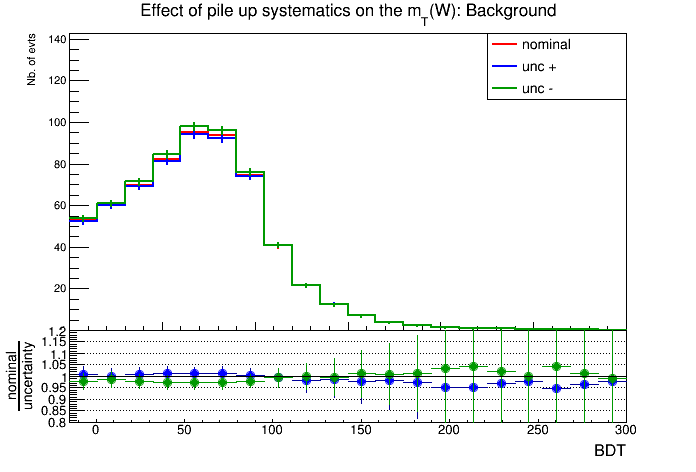
\includegraphics[width=0.48\textwidth]{Figures/boosteddecisiontrees/MTWsys/hist_mWt_puSF_nom_bkg}
	\caption{Distribution of the nominal values and shift due to pile up uncertainties for the transverse mass of the \PW\ boson in the \WZCR. All channel.}
	\label{fig:pileupshiftmtWSTzct}
\end{figure}
\begin{figure}[h] 
	\centering
	% \subfigure[Background]{% \includegraphics[width=0.48\textwidth]{Figures/boosteddecisiontrees/singletopzct/systematics/hist_BDT_puSF_nom_bkg}}
	% \subfigure[Signal]{% \includegraphics[width=0.48\textwidth]{Figures/boosteddecisiontrees/singletopzct/systematics/hist_BDT_puSF_nom_sig}}
	\caption{Distribution of the nominal values and shift due to pile up uncertainties for the BDT discriminant for the \Zct\ vertex in the \STSR. All channel.}
	\label{fig:pileupshiftBDTSTzct}
\end{figure}
\begin{figure}[h] 
	\centering
	% \subfigure[Background]{% \includegraphics[width=0.48\textwidth]{Figures/boosteddecisiontrees/singletopzut/systematics/hist_BDT_puSF_nom_bkg}}
	% \subfigure[Signal]{% \includegraphics[width=0.48\textwidth]{Figures/boosteddecisiontrees/singletopzut/systematics/hist_BDT_puSF_nom_sig}}
	\caption{Distribution of the nominal values and shift due to pile up uncertainties for the BDT discriminant for the \Zut\ vertex in the \STSR. All channel.}
	\label{fig:pileupshiftBDTSTzut}
\end{figure}
\begin{figure}[h] 
	\centering
	% \subfigure[Background]{% \includegraphics[width=0.48\textwidth]{Figures/boosteddecisiontrees/toppairzct/systematics/hist_BDT_puSF_nom_bkg}}
	% \subfigure[Signal]{% \includegraphics[width=0.48\textwidth]{Figures/boosteddecisiontrees/toppairzct/systematics/hist_BDT_puSF_nom_sig}}
	\caption{Distribution of the nominal values and shift due to pile up uncertainties for the BDT discriminant for the \Zct\ vertex in the \TTSR. All channel.}
	\label{fig:pileupshiftBDTTTzct}
\end{figure}
\begin{figure}[h] 
	\centering
	% \subfigure[Background]{% \includegraphics[width=0.48\textwidth]{Figures/boosteddecisiontrees/toppairzut/systematics/hist_BDT_puSF_nom_bkg}}
	% \subfigure[Signal]{% \includegraphics[width=0.48\textwidth]{Figures/boosteddecisiontrees/toppairzut/systematics/hist_BDT_puSF_nom_sig}}
	\caption{Distribution of the nominal values and shift due to pile up uncertainties for the BDT discriminant for the \Zut\ vertex in the \TTSR. All channel.}
	\label{fig:pileupshiftBDTTTzut}
\end{figure}


\subsection{Effect of electron scale factors on the shapes}
\label{sec:electronsys}

\begin{figure}[h] 
	\centering
	% 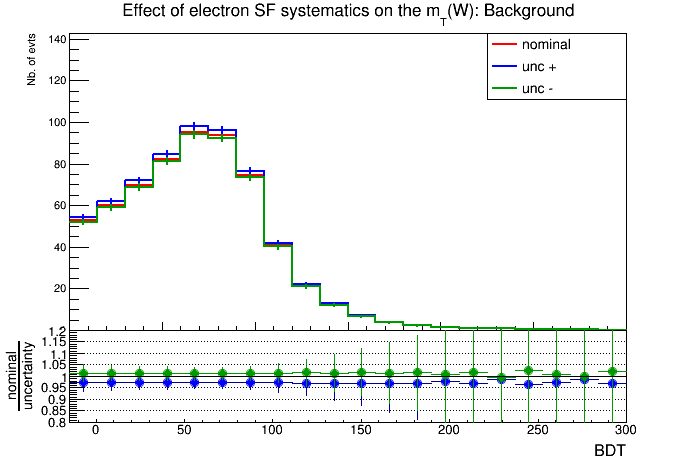
\includegraphics[width=0.48\textwidth]{Figures/boosteddecisiontrees/MTWsys/hist_mWt_electronSF_nom_bkg}
	\caption{Distribution of the nominal values and shift due to electron scale factors uncertainties for the transverse mass of the \PW\ boson in the \WZCR. All channel.}
	\label{fig:electronsfshiftmtWSTzct}
\end{figure}
\begin{figure}[h] 
	\centering
	% \subfigure[Background]{% \includegraphics[width=0.48\textwidth]{Figures/boosteddecisiontrees/singletopzct/systematics/hist_BDT_electronSF_nom_bkg}}
	% \subfigure[Signal]{% \includegraphics[width=0.48\textwidth]{Figures/boosteddecisiontrees/singletopzct/systematics/hist_BDT_electronSF_nom_sig}}
	\caption{Distribution of the nominal values and shift due to electron scale factor uncertainties for the BDT discriminant for the \Zct\ vertex in the \STSR. All channel.}
	\label{fig:electronsfshiftBDTSTzct}
\end{figure}
\begin{figure}[h] 
	\centering
	% \subfigure[Background]{% \includegraphics[width=0.48\textwidth]{Figures/boosteddecisiontrees/singletopzut/systematics/hist_BDT_electronSF_nom_bkg}}
	% \subfigure[Signal]{% \includegraphics[width=0.48\textwidth]{Figures/boosteddecisiontrees/singletopzut/systematics/hist_BDT_electronSF_nom_sig}}
	\caption{Distribution of the nominal values and shift due to electron scale factor uncertainties for the BDT discriminant for the \Zut\ vertex in the \STSR. All channel.}
	\label{fig:electronsfshiftBDTSTzut}
\end{figure}
\begin{figure}[h] 
	\centering
	% \subfigure[Background]{% \includegraphics[width=0.48\textwidth]{Figures/boosteddecisiontrees/toppairzct/systematics/hist_BDT_electronSF_nom_bkg}}
	% \subfigure[Signal]{% \includegraphics[width=0.48\textwidth]{Figures/boosteddecisiontrees/toppairzct/systematics/hist_BDT_electronSF_nom_sig}}
	\caption{Distribution of the nominal values and shift due to electron scale factor uncertainties for the BDT discriminant for the \Zct\ vertex in the \TTSR. All channel.}
	\label{fig:electronsfshiftBDTTTzct}
\end{figure}
\begin{figure}[h] 
	\centering
	% \subfigure[Background]{% \includegraphics[width=0.48\textwidth]{Figures/boosteddecisiontrees/toppairzut/systematics/hist_BDT_electronSF_nom_bkg}}
	% \subfigure[Signal]{% \includegraphics[width=0.48\textwidth]{Figures/boosteddecisiontrees/toppairzut/systematics/hist_BDT_electronSF_nom_sig}}
	\caption{Distribution of the nominal values and shift due to electron scale factor uncertainties for the BDT discriminant for the \Zut\ vertex in the \TTSR. All channel.}
	\label{fig:electronsfshiftBDTTTzut}
\end{figure}


\subsection{Effect of muon scale factors on the shapes}
\label{sec:muonsys}
\begin{figure}[h] 
	\centering
	% 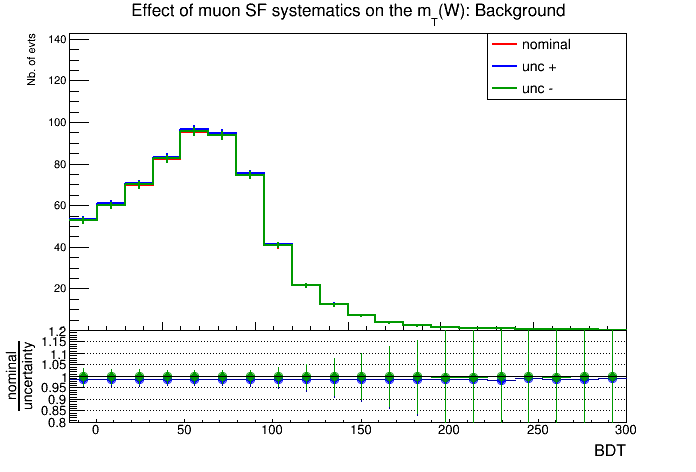
\includegraphics[width=0.48\textwidth]{Figures/boosteddecisiontrees/MTWsys/hist_mWt_muonSF_nom_bkg}
	\caption{Distribution of the nominal values and shift due to muon scale factors uncertainties for the transverse mass of the \PW\ boson in the \WZCR. All channel.}
	\label{fig:muonsfshiftmtWSTzct}
\end{figure}
\begin{figure}[h] 
	\centering
	% \subfigure[Background]{% \includegraphics[width=0.48\textwidth]{Figures/boosteddecisiontrees/singletopzct/systematics/hist_BDT_muonSF_nom_bkg}}
	% \subfigure[Signal]{% \includegraphics[width=0.48\textwidth]{Figures/boosteddecisiontrees/singletopzct/systematics/hist_BDT_muonSF_nom_sig}}
	\caption{Distribution of the nominal values and shift due to muon scale factor uncertainties for the BDT discriminant for the \Zct\ vertex in the \STSR. All channel.}
	\label{fig:muonsfshiftBDTSTzct}
\end{figure}
\begin{figure}[h] 
	\centering
	% \subfigure[Background]{% \includegraphics[width=0.48\textwidth]{Figures/boosteddecisiontrees/singletopzut/systematics/hist_BDT_muonSF_nom_bkg}}
	% \subfigure[Signal]{% \includegraphics[width=0.48\textwidth]{Figures/boosteddecisiontrees/singletopzut/systematics/hist_BDT_muonSF_nom_sig}}
	\caption{Distribution of the nominal values and shift due to muon scale factor uncertainties for the BDT discriminant for the \Zut\ vertex in the \STSR. All channel.}
	\label{fig:muonsfshiftBDTSTzut}
\end{figure}
\begin{figure}[h] 
	\centering
	% \subfigure[Background]{% \includegraphics[width=0.48\textwidth]{Figures/boosteddecisiontrees/toppairzct/systematics/hist_BDT_muonSF_nom_bkg}}
	% \subfigure[Signal]{% \includegraphics[width=0.48\textwidth]{Figures/boosteddecisiontrees/toppairzct/systematics/hist_BDT_muonSF_nom_sig}}
	\caption{Distribution of the nominal values and shift due to muon scale factor uncertainties for the BDT discriminant for the \Zct\ vertex in the \TTSR. All channel.}
	\label{fig:muonsfshiftBDTTTzct}
\end{figure}
\begin{figure}[h] 
	\centering
	% \subfigure[Background]{% \includegraphics[width=0.48\textwidth]{Figures/boosteddecisiontrees/toppairzut/systematics/hist_BDT_muonSF_nom_bkg}}
	% \subfigure[Signal]{% \includegraphics[width=0.48\textwidth]{Figures/boosteddecisiontrees/toppairzut/systematics/hist_BDT_muonSF_nom_sig}}
	\caption{Distribution of the nominal values and shift due to muon scale factor uncertainties for the BDT discriminant for the \Zut\ vertex in the \TTSR. All channel.}
	\label{fig:muonsfshiftBDTTTzut}
\end{figure}


\subsection{Effect of JES on the shapes}
\label{sec:JESsys}
\begin{figure}[h] 
	\centering 
	% 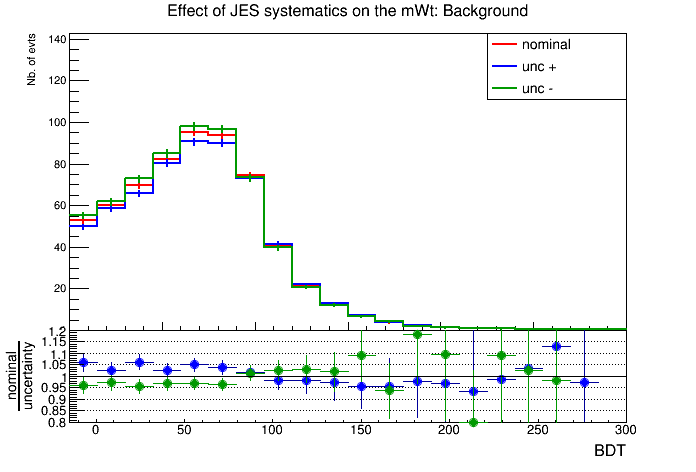
\includegraphics[width=0.48\textwidth]{Figures/boosteddecisiontrees/MTWsys/hist_mWt_JES_nom_bkg}
	\caption{Distribution of the nominal values and shift due to JES uncertainties for the transverse mass of the \PW\ boson in the \WZCR. All channel.}
	\label{fig:JESshiftmtWSTzct}
\end{figure}
\begin{figure}[h] 
	\centering
	% \subfigure[Background]{% \includegraphics[width=0.48\textwidth]{Figures/boosteddecisiontrees/singletopzct/systematics/hist_BDT_JES_nom_bkg}}
	% \subfigure[Signal]{% \includegraphics[width=0.48\textwidth]{Figures/boosteddecisiontrees/singletopzct/systematics/hist_BDT_JES_nom_sig}}
	\caption{Distribution of the nominal values and shift due to JES uncertainties for the BDT discriminant for the \Zct\ vertex in the \STSR. All channel.}
	\label{fig:JESshiftBDTSTzct}
\end{figure}
\begin{figure}[h] 
	\centering
	% \subfigure[Background]{% \includegraphics[width=0.48\textwidth]{Figures/boosteddecisiontrees/singletopzut/systematics/hist_BDT_JES_nom_bkg}}
	% \subfigure[Signal]{% \includegraphics[width=0.48\textwidth]{Figures/boosteddecisiontrees/singletopzut/systematics/hist_BDT_JES_nom_sig}}
	\caption{Distribution of the nominal values and shift due to JES uncertainties for the BDT discriminant for the \Zut\ vertex in the \STSR. All channel.}
	\label{fig:JESshiftBDTSTzut}
\end{figure}
\begin{figure}[h] 
	\centering
	% \subfigure[Background]{% \includegraphics[width=0.48\textwidth]{Figures/boosteddecisiontrees/toppairzct/systematics/hist_BDT_JES_nom_bkg}}
	% \subfigure[Signal]{% \includegraphics[width=0.48\textwidth]{Figures/boosteddecisiontrees/toppairzct/systematics/hist_BDT_JES_nom_sig}}
	\caption{Distribution of the nominal values and shift due to JES uncertainties for the BDT discriminant for the \Zct\ vertex in the \TTSR. All channel.}
	\label{fig:JESshiftBDTTTzct}
\end{figure}
\begin{figure}[h] 
	\centering
	% \subfigure[Background]{% \includegraphics[width=0.48\textwidth]{Figures/boosteddecisiontrees/toppairzut/systematics/hist_BDT_JES_nom_bkg}}
	% \subfigure[Signal]{% \includegraphics[width=0.48\textwidth]{Figures/boosteddecisiontrees/toppairzut/systematics/hist_BDT_JES_nom_sig}}
	\caption{Distribution of the nominal values and shift due to JES uncertainties for the BDT discriminant for the \Zut\ vertex in the \TTSR. All channel.}
	\label{fig:JESshiftBDTTTzut}
\end{figure}


\subsection{Effect of JER on the shapes}
\label{sec:JERsys}
\begin{figure}[h] 
	\centering 
	% \includegraphics[width=0.48\textwidth]{Figures/boosteddecisiontrees/MTWsys/hist_mWt_JER_nom_bkg}
	\caption{Distribution of the nominal values and shift due to JER uncertainties for the transverse mass of the \PW\ boson in the \WZCR. All channel.}
	\label{fig:JERshiftmtWSTzct}
\end{figure}
\begin{figure}[h] 
	\centering
	% \subfigure[Background]{% \includegraphics[width=0.48\textwidth]{Figures/boosteddecisiontrees/singletopzct/systematics/hist_BDT_JER_nom_bkg}}
	% \subfigure[Signal]{% \includegraphics[width=0.48\textwidth]{Figures/boosteddecisiontrees/singletopzct/systematics/hist_BDT_JER_nom_sig}}
	\caption{Distribution of the nominal values and shift due to JER uncertainties for the BDT discriminant for the \Zct\ vertex in the \STSR. All channel.}
	\label{fig:JERshiftBDTSTzct}
\end{figure}
\begin{figure}[h] 
	\centering
	% \subfigure[Background]{% \includegraphics[width=0.48\textwidth]{Figures/boosteddecisiontrees/singletopzut/systematics/hist_BDT_JER_nom_bkg}}
	% \subfigure[Signal]{% \includegraphics[width=0.48\textwidth]{Figures/boosteddecisiontrees/singletopzut/systematics/hist_BDT_JER_nom_sig}}
	\caption{Distribution of the nominal values and shift due to JER uncertainties for the BDT discriminant for the \Zut\ vertex in the \STSR. All channel.}
	\label{fig:JERshiftBDTSTzut}
\end{figure}
\begin{figure}[h] 
	\centering
	% \subfigure[Background]{% \includegraphics[width=0.48\textwidth]{Figures/boosteddecisiontrees/toppairzct/systematics/hist_BDT_JER_nom_bkg}}
	% \subfigure[Signal]{% \includegraphics[width=0.48\textwidth]{Figures/boosteddecisiontrees/toppairzct/systematics/hist_BDT_JER_nom_sig}}
	\caption{Distribution of the nominal values and shift due to JER uncertainties for the BDT discriminant for the \Zct\ vertex in the \TTSR. All channel.}
	\label{fig:JERshiftBDTTTzct}
\end{figure}
\begin{figure}[h] 
	\centering
	% \subfigure[Background]{% \includegraphics[width=0.48\textwidth]{Figures/boosteddecisiontrees/toppairzut/systematics/hist_BDT_JER_nom_bkg}}
	% \subfigure[Signal]{% \includegraphics[width=0.48\textwidth]{Figures/boosteddecisiontrees/toppairzut/systematics/hist_BDT_JER_nom_sig}}
	\caption{Distribution of the nominal values and shift due to JER uncertainties for the BDT discriminant for the \Zut\ vertex in the \TTSR. All channel.}
	\label{fig:JERshiftBDTTTzut}
\end{figure}



\subsection{Effect of b-tag scale factors on the shapes}
\label{sec:btagsys}
\begin{figure}[h] 
	\centering
	% \includegraphics[width=0.48\textwidth]{Figures/boosteddecisiontrees/MTWsys/hist_mWt_btagSF_cferr1_nom_bkg}
	\caption{Distribution of the nominal values and shift due to b tag cferr1 scale factors uncertainties for the transverse mass of the \PW\ boson in the \WZCR. All channel.}
	\label{fig:btagcferr1shiftmtWSTzct}
\end{figure}
\begin{figure}[h] 
	\centering
	% \subfigure[Background]{% \includegraphics[width=0.48\textwidth]{Figures/boosteddecisiontrees/singletopzct/systematics/hist_BDT_btagSF_cferr1_nom_bkg}}
	% \subfigure[Signal]{% \includegraphics[width=0.48\textwidth]{Figures/boosteddecisiontrees/singletopzct/systematics/hist_BDT_btagSF_cferr1_nom_sig}}
	\caption{Distribution of the nominal values and shift due to b tag cferr1 scale factor uncertainties for the BDT discriminant for the \Zct\ vertex in the \STSR. All channel.}
	\label{fig:btag_cferr1sfshiftBDTSTzct}
\end{figure}

\begin{figure}[h] 
	\centering
	% \subfigure[Background]{% \includegraphics[width=0.48\textwidth]{Figures/boosteddecisiontrees/singletopzut/systematics/hist_BDT_btagSF_cferr1_nom_bkg}}
	% \subfigure[Signal]{% \includegraphics[width=0.48\textwidth]{Figures/boosteddecisiontrees/singletopzut/systematics/hist_BDT_btagSF_cferr1_nom_sig}}
	\caption{Distribution of the nominal values and shift due to b tag cferr1 scale factor uncertainties for the BDT discriminant for the \Zut\ vertex in the \STSR. All channel.}
	\label{fig:btag_cferr1sfshiftBDTSTzut}
\end{figure}


\begin{figure}[h] 
	\centering
	% \subfigure[Background]{% \includegraphics[width=0.48\textwidth]{Figures/boosteddecisiontrees/toppairzct/systematics/hist_BDT_btagSF_cferr1_nom_bkg}}
	% \subfigure[Signal]{% \includegraphics[width=0.48\textwidth]{Figures/boosteddecisiontrees/toppairzct/systematics/hist_BDT_btagSF_cferr1_nom_sig}}
	\caption{Distribution of the nominal values and shift due to b tag cferr1 scale factor uncertainties for the BDT discriminant for the \Zct\ vertex in the \TTSR. All channel.}
	\label{fig:btag_cferr1sfshiftBDTTTzct}
\end{figure}


\begin{figure}[h] 
	\centering
	% \subfigure[Background]{% \includegraphics[width=0.48\textwidth]{Figures/boosteddecisiontrees/toppairzut/systematics/hist_BDT_btagSF_cferr1_nom_bkg}}
	% \subfigure[Signal]{% \includegraphics[width=0.48\textwidth]{Figures/boosteddecisiontrees/toppairzut/systematics/hist_BDT_btagSF_cferr1_nom_sig}}
	\caption{Distribution of the nominal values and shift due to b tag cferr1 scale factor uncertainties for the BDT discriminant for the \Zut\ vertex in the \TTSR. All channel.}
	\label{fig:btag_cferr1sfshiftBDTTTzut}
\end{figure}

\begin{figure}[h] 
	\centering
	% \includegraphics[width=0.48\textwidth]{Figures/boosteddecisiontrees/MTWsys/hist_mWt_btagSF_cferr2_nom_bkg}
	\caption{Distribution of the nominal values and shift due to b tag cferr2 scale factors uncertainties for the transverse mass of the \PW\ boson in the \WZCR. All channel.}
	\label{fig:btagcferr2shiftmtWSTzct}
\end{figure}

\begin{figure}[h] 
	\centering
	% \subfigure[Background]{% \includegraphics[width=0.48\textwidth]{Figures/boosteddecisiontrees/singletopzct/systematics/hist_BDT_btagSF_cferr2_nom_bkg}}
	% \subfigure[Signal]{% \includegraphics[width=0.48\textwidth]{Figures/boosteddecisiontrees/singletopzct/systematics/hist_BDT_btagSF_cferr2_nom_sig}}
	\caption{Distribution of the nominal values and shift due to b tag cferr2 scale factor uncertainties for the BDT discriminant for the \Zct\ vertex in the \STSR. All channel.}
	\label{fig:btag_cferr2sfshiftBDTSTzct}
\end{figure}


\begin{figure}[h] 
	\centering
	% \subfigure[Background]{% \includegraphics[width=0.48\textwidth]{Figures/boosteddecisiontrees/singletopzut/systematics/hist_BDT_btagSF_cferr2_nom_bkg}}
	% \subfigure[Signal]{% \includegraphics[width=0.48\textwidth]{Figures/boosteddecisiontrees/singletopzut/systematics/hist_BDT_btagSF_cferr2_nom_sig}}
	\caption{Distribution of the nominal values and shift due to b tag cferr2 scale factor uncertainties for the BDT discriminant for the \Zut\ vertex in the \STSR. All channel.}
	\label{fig:btag_cferr2sfshiftBDTSTzut}
\end{figure}

\begin{figure}[h] 
	\centering
	% \subfigure[Background]{% \includegraphics[width=0.48\textwidth]{Figures/boosteddecisiontrees/toppairzct/systematics/hist_BDT_btagSF_cferr2_nom_bkg}}
	% \subfigure[Signal]{% \includegraphics[width=0.48\textwidth]{Figures/boosteddecisiontrees/toppairzct/systematics/hist_BDT_btagSF_cferr2_nom_sig}}
	\caption{Distribution of the nominal values and shift due to b tag cferr2 scale factor uncertainties for the BDT discriminant for the \Zct\ vertex in the \TTSR. All channel.}
	\label{fig:btag_cferr2sfshiftBDTTTzct}
\end{figure}

\begin{figure}[h] 
	\centering
	% \subfigure[Background]{% \includegraphics[width=0.48\textwidth]{Figures/boosteddecisiontrees/toppairzut/systematics/hist_BDT_btagSF_cferr2_nom_bkg}}
	% \subfigure[Signal]{% \includegraphics[width=0.48\textwidth]{Figures/boosteddecisiontrees/toppairzut/systematics/hist_BDT_btagSF_cferr2_nom_sig}}
	\caption{Distribution of the nominal values and shift due to b tag cferr2 scale factor uncertainties for the BDT discriminant for the \Zut\ vertex in the \TTSR. All channel.}
	\label{fig:btag_cferr2sfshiftBDTTTzut}
\end{figure}

\begin{figure}[h] 
	\centering
	% \includegraphics[width=0.48\textwidth]{Figures/boosteddecisiontrees/MTWsys/hist_mWt_btagSF_hf_nom_bkg}
	\caption{Distribution of the nominal values and shift due to b tag hf scale factors uncertainties for the transverse mass of the \PW\ boson in the \WZCR. All channel.}
	\label{fig:btaghfshiftmtWSTzct}
\end{figure}
\begin{figure}[h] 
	\centering
	% \subfigure[Background]{% \includegraphics[width=0.48\textwidth]{Figures/boosteddecisiontrees/singletopzct/systematics/hist_BDT_btagSF_hf_nom_bkg}}
	% \subfigure[Signal]{% \includegraphics[width=0.48\textwidth]{Figures/boosteddecisiontrees/singletopzct/systematics/hist_BDT_btagSF_hf_nom_sig}}
	\caption{Distribution of the nominal values and shift due to b tag hf scale factor uncertainties for the BDT discriminant for the \Zct\ vertex in the \STSR. All channel.}
	\label{fig:btag_hfsfshiftBDTSTzct}
\end{figure}

\begin{figure}[h] 
	\centering
	% \subfigure[Background]{% \includegraphics[width=0.48\textwidth]{Figures/boosteddecisiontrees/singletopzut/systematics/hist_BDT_btagSF_hf_nom_bkg}}
	% \subfigure[Signal]{% \includegraphics[width=0.48\textwidth]{Figures/boosteddecisiontrees/singletopzut/systematics/hist_BDT_btagSF_hf_nom_sig}}
	\caption{Distribution of the nominal values and shift due to b tag hf scale factor uncertainties for the BDT discriminant for the \Zut\ vertex in the \STSR. All channel.}
	\label{fig:btag_hfsfshiftBDTSTzut}
\end{figure}

\begin{figure}[h] 
	\centering
	% \subfigure[Background]{% \includegraphics[width=0.48\textwidth]{Figures/boosteddecisiontrees/toppairzct/systematics/hist_BDT_btagSF_hf_nom_bkg}}
	% \subfigure[Signal]{% \includegraphics[width=0.48\textwidth]{Figures/boosteddecisiontrees/toppairzct/systematics/hist_BDT_btagSF_hf_nom_sig}}
	\caption{Distribution of the nominal values and shift due to b tag hf scale factor uncertainties for the BDT discriminant for the \Zct\ vertex in the \TTSR. All channel.}
	\label{fig:btag_hfsfshiftBDTTTzct}
\end{figure}

\begin{figure}[h] 
	\centering
	% \subfigure[Background]{% \includegraphics[width=0.48\textwidth]{Figures/boosteddecisiontrees/toppairzut/systematics/hist_BDT_btagSF_hf_nom_bkg}}
	% \subfigure[Signal]{% \includegraphics[width=0.48\textwidth]{Figures/boosteddecisiontrees/toppairzut/systematics/hist_BDT_btagSF_hf_nom_sig}}
	\caption{Distribution of the nominal values and shift due to b tag hf scale factor uncertainties for the BDT discriminant for the \Zut\ vertex in the \TTSR. All channel.}
	\label{fig:btag_hfsfshiftBDTTTzut}
\end{figure}
\begin{figure}[h] 
	\centering
	% \includegraphics[width=0.48\textwidth]{Figures/boosteddecisiontrees/MTWsys/hist_mWt_btagSF_hfstats1_nom_bkg}
	\caption{Distribution of the nominal values and shift due to b tag hfstats1 scale factors uncertainties for the transverse mass of the \PW\ boson in the \WZCR. All channel.}
	\label{fig:btaghfstats1shiftmtWSTzct}
\end{figure}
\begin{figure}[h] 
	\centering
	% \subfigure[Background]{% \includegraphics[width=0.48\textwidth]{Figures/boosteddecisiontrees/singletopzct/systematics/hist_BDT_btagSF_hfstats1_nom_bkg}}
	% \subfigure[Signal]{% \includegraphics[width=0.48\textwidth]{Figures/boosteddecisiontrees/singletopzct/systematics/hist_BDT_btagSF_hfstats1_nom_sig}}
	\caption{Distribution of the nominal values and shift due to b tag hfstats1 scale factor uncertainties for the BDT discriminant for the \Zct\ vertex in the \STSR. All channel.}
	\label{fig:btag_hfstats1sfshiftBDTSTzct}
\end{figure}

\begin{figure}[h] 
	\centering
	% \subfigure[Background]{% \includegraphics[width=0.48\textwidth]{Figures/boosteddecisiontrees/singletopzut/systematics/hist_BDT_btagSF_hfstats1_nom_bkg}}
	% \subfigure[Signal]{% \includegraphics[width=0.48\textwidth]{Figures/boosteddecisiontrees/singletopzut/systematics/hist_BDT_btagSF_hfstats1_nom_sig}}
	\caption{Distribution of the nominal values and shift due to b tag hfstats1 scale factor uncertainties for the BDT discriminant for the \Zut\ vertex in the \STSR. All channel.}
	\label{fig:btag_hfstats1sfshiftBDTSTzut}
\end{figure}

\begin{figure}[h] 
	\centering
	% \subfigure[Background]{% \includegraphics[width=0.48\textwidth]{Figures/boosteddecisiontrees/toppairzct/systematics/hist_BDT_btagSF_hfstats1_nom_bkg}}
	% \subfigure[Signal]{% \includegraphics[width=0.48\textwidth]{Figures/boosteddecisiontrees/toppairzct/systematics/hist_BDT_btagSF_hfstats1_nom_sig}}
	\caption{Distribution of the nominal values and shift due to b tag hfstats1 scale factor uncertainties for the BDT discriminant for the \Zct\ vertex in the \TTSR. All channel.}
	\label{fig:btag_hfstats1sfshiftBDTTTzct}
\end{figure}

\begin{figure}[h] 
	\centering
	% \subfigure[Background]{% \includegraphics[width=0.48\textwidth]{Figures/boosteddecisiontrees/toppairzut/systematics/hist_BDT_btagSF_hfstats1_nom_bkg}}
	% \subfigure[Signal]{% \includegraphics[width=0.48\textwidth]{Figures/boosteddecisiontrees/toppairzut/systematics/hist_BDT_btagSF_hfstats1_nom_sig}}
	\caption{Distribution of the nominal values and shift due to b tag hfstats1 scale factor uncertainties for the BDT discriminant for the \Zut\ vertex in the \TTSR. All channel.}
	\label{fig:btag_hfstats1sfshiftBDTTTzut}
\end{figure}
\begin{figure}[h] 
	\centering
	% \includegraphics[width=0.48\textwidth]{Figures/boosteddecisiontrees/MTWsys/hist_mWt_btagSF_hfstats2_nom_bkg}
	\caption{Distribution of the nominal values and shift due to b tag hfstats2 scale factors uncertainties for the transverse mass of the \PW\ boson in the \WZCR. All channel.}
	\label{fig:btaghfstats2shiftmtWSTzct}
\end{figure}
\begin{figure}[h] 
	\centering
	% \subfigure[Background]{% \includegraphics[width=0.48\textwidth]{Figures/boosteddecisiontrees/singletopzct/systematics/hist_BDT_btagSF_hfstats2_nom_bkg}}
	% \subfigure[Signal]{% \includegraphics[width=0.48\textwidth]{Figures/boosteddecisiontrees/singletopzct/systematics/hist_BDT_btagSF_hfstats2_nom_sig}}
	\caption{Distribution of the nominal values and shift due to b tag hfstats2 scale factor uncertainties for the BDT discriminant for the \Zct\ vertex in the \STSR. All channel.}
	\label{fig:btag_hfstats2sfshiftBDTSTzct}
\end{figure}

\begin{figure}[h] 
	\centering
	% \subfigure[Background]{% \includegraphics[width=0.48\textwidth]{Figures/boosteddecisiontrees/singletopzut/systematics/hist_BDT_btagSF_hfstats2_nom_bkg}}
	% \subfigure[Signal]{% \includegraphics[width=0.48\textwidth]{Figures/boosteddecisiontrees/singletopzut/systematics/hist_BDT_btagSF_hfstats2_nom_sig}}
	\caption{Distribution of the nominal values and shift due to b tag hfstats2 scale factor uncertainties for the BDT discriminant for the \Zut\ vertex in the \STSR. All channel.}
	\label{fig:btag_hfstats2sfshiftBDTSTzut}
\end{figure}

\begin{figure}[h] 
	\centering
	% \subfigure[Background]{% \includegraphics[width=0.48\textwidth]{Figures/boosteddecisiontrees/toppairzct/systematics/hist_BDT_btagSF_hfstats2_nom_bkg}}
	% \subfigure[Signal]{% \includegraphics[width=0.48\textwidth]{Figures/boosteddecisiontrees/toppairzct/systematics/hist_BDT_btagSF_hfstats2_nom_sig}}
	\caption{Distribution of the nominal values and shift due to b tag hfstats2 scale factor uncertainties for the BDT discriminant for the \Zct\ vertex in the \TTSR. All channel.}
	\label{fig:btag_hfstats2sfshiftBDTTTzct}
\end{figure}

\begin{figure}[h] 
	\centering
	% \subfigure[Background]{% \includegraphics[width=0.48\textwidth]{Figures/boosteddecisiontrees/toppairzut/systematics/hist_BDT_btagSF_hfstats2_nom_bkg}}
	% \subfigure[Signal]{% \includegraphics[width=0.48\textwidth]{Figures/boosteddecisiontrees/toppairzut/systematics/hist_BDT_btagSF_hfstats2_nom_sig}}
	\caption{Distribution of the nominal values and shift due to b tag hfstats2 scale factor uncertainties for the BDT discriminant for the \Zut\ vertex in the \TTSR. All channel.}
	\label{fig:btag_hfstats2sfshiftBDTTTzut}
\end{figure}



\begin{figure}[h] 
	\centering
	% \includegraphics[width=0.48\textwidth]{Figures/boosteddecisiontrees/MTWsys/hist_mWt_btagSF_lf_nom_bkg}
	\caption{Distribution of the nominal values and shift due to b tag lf scale factors uncertainties for the transverse mass of the \PW\ boson in the \WZCR. All channel.}
	\label{fig:btaglfshiftmtWSTzct}
\end{figure}
\begin{figure}[h] 
	\centering
	% \subfigure[Background]{% \includegraphics[width=0.48\textwidth]{Figures/boosteddecisiontrees/singletopzct/systematics/hist_BDT_btagSF_lf_nom_bkg}}
	% \subfigure[Signal]{% \includegraphics[width=0.48\textwidth]{Figures/boosteddecisiontrees/singletopzct/systematics/hist_BDT_btagSF_lf_nom_sig}}
	\caption{Distribution of the nominal values and shift due to b tag lf scale factor uncertainties for the BDT discriminant for the \Zct\ vertex in the \STSR. All channel.}
	\label{fig:btag_lfsfshiftBDTSTzct}
\end{figure}

\begin{figure}[h] 
	\centering
	% \subfigure[Background]{% \includegraphics[width=0.48\textwidth]{Figures/boosteddecisiontrees/singletopzut/systematics/hist_BDT_btagSF_lf_nom_bkg}}
	% \subfigure[Signal]{% \includegraphics[width=0.48\textwidth]{Figures/boosteddecisiontrees/singletopzut/systematics/hist_BDT_btagSF_lf_nom_sig}}
	\caption{Distribution of the nominal values and shift due to b tag lf scale factor uncertainties for the BDT discriminant for the \Zut\ vertex in the \STSR. All channel.}
	\label{fig:btag_lfsfshiftBDTSTzut}
\end{figure}

\begin{figure}[h] 
	\centering
	% \subfigure[Background]{% \includegraphics[width=0.48\textwidth]{Figures/boosteddecisiontrees/toppairzct/systematics/hist_BDT_btagSF_lf_nom_bkg}}
	% \subfigure[Signal]{% \includegraphics[width=0.48\textwidth]{Figures/boosteddecisiontrees/toppairzct/systematics/hist_BDT_btagSF_lf_nom_sig}}
	\caption{Distribution of the nominal values and shift due to b tag lf scale factor uncertainties for the BDT discriminant for the \Zct\ vertex in the \TTSR. All channel.}
	\label{fig:btag_lfsfshiftBDTTTzct}
\end{figure}


\begin{figure}[h] 
	\centering
	% \subfigure[Background]{% \includegraphics[width=0.48\textwidth]{Figures/boosteddecisiontrees/toppairzut/systematics/hist_BDT_btagSF_lf_nom_bkg}}
	% \subfigure[Signal]{% \includegraphics[width=0.48\textwidth]{Figures/boosteddecisiontrees/toppairzut/systematics/hist_BDT_btagSF_lf_nom_sig}}
	\caption{Distribution of the nominal values and shift due to b tag lf scale factor uncertainties for the BDT discriminant for the \Zut\ vertex in the \TTSR. All channel.}
	\label{fig:btag_lfsfshiftBDTTTzut}
\end{figure}
\begin{figure}[h] 
	\centering
	% \includegraphics[width=0.48\textwidth]{Figures/boosteddecisiontrees/MTWsys/hist_mWt_btagSF_lfstats1_nom_bkg}
	\caption{Distribution of the nominal values and shift due to b tag lfstats1 scale factors uncertainties for the transverse mass of the \PW\ boson in the \WZCR. All channel.}
	\label{fig:btaglfstats1shiftmtWSTzct}
\end{figure}
\begin{figure}[h] 
	\centering
	% \subfigure[Background]{% \includegraphics[width=0.48\textwidth]{Figures/boosteddecisiontrees/singletopzct/systematics/hist_BDT_btagSF_lfstats1_nom_bkg}}
	% \subfigure[Signal]{% \includegraphics[width=0.48\textwidth]{Figures/boosteddecisiontrees/singletopzct/systematics/hist_BDT_btagSF_lfstats1_nom_sig}}
	\caption{Distribution of the nominal values and shift due to b tag lfstats1 scale factor uncertainties for the BDT discriminant for the \Zct\ vertex in the \STSR. All channel.}
	\label{fig:btag_lfstats1sfshiftBDTSTzct}
\end{figure}

\begin{figure}[h] 
	\centering
	% \subfigure[Background]{% \includegraphics[width=0.48\textwidth]{Figures/boosteddecisiontrees/singletopzut/systematics/hist_BDT_btagSF_lfstats1_nom_bkg}}
	% \subfigure[Signal]{% \includegraphics[width=0.48\textwidth]{Figures/boosteddecisiontrees/singletopzut/systematics/hist_BDT_btagSF_lfstats1_nom_sig}}
	\caption{Distribution of the nominal values and shift due to b tag lfstats1 scale factor uncertainties for the BDT discriminant for the \Zut\ vertex in the \STSR. All channel.}
	\label{fig:btag_lfstats1sfshiftBDTSTzut}
\end{figure}

\begin{figure}[h] 
	\centering
	% \subfigure[Background]{% \includegraphics[width=0.48\textwidth]{Figures/boosteddecisiontrees/toppairzct/systematics/hist_BDT_btagSF_lfstats1_nom_bkg}}
	% \subfigure[Signal]{% \includegraphics[width=0.48\textwidth]{Figures/boosteddecisiontrees/toppairzct/systematics/hist_BDT_btagSF_lfstats1_nom_sig}}
	\caption{Distribution of the nominal values and shift due to b tag lfstats1 scale factor uncertainties for the BDT discriminant for the \Zct\ vertex in the \TTSR. All channel.}
	\label{fig:btag_lfstats1sfshiftBDTTTzct}
\end{figure}

\begin{figure}[h] 
	\centering
	% \subfigure[Background]{% \includegraphics[width=0.48\textwidth]{Figures/boosteddecisiontrees/toppairzut/systematics/hist_BDT_btagSF_lfstats1_nom_bkg}}
	% \subfigure[Signal]{% \includegraphics[width=0.48\textwidth]{Figures/boosteddecisiontrees/toppairzut/systematics/hist_BDT_btagSF_lfstats1_nom_sig}}
	\caption{Distribution of the nominal values and shift due to b tag lfstats1 scale factor uncertainties for the BDT discriminant for the \Zut\ vertex in the \TTSR. All channel.}
	\label{fig:btag_lfstats1sfshiftBDTTTzut}
\end{figure}
\begin{figure}[h] 
	\centering
	% \includegraphics[width=0.48\textwidth]{Figures/boosteddecisiontrees/MTWsys/hist_mWt_btagSF_lfstats2_nom_bkg}
	\caption{Distribution of the nominal values and shift due to b tag lfstats2 scale factors uncertainties for the transverse mass of the \PW\ boson in the \WZCR. All channel.}
	\label{fig:btaglfstats2shiftmtWSTzct}
\end{figure}
\begin{figure}[h] 
	\centering
	% \subfigure[Background]{% \includegraphics[width=0.48\textwidth]{Figures/boosteddecisiontrees/singletopzct/systematics/hist_BDT_btagSF_lfstats2_nom_bkg}}
	% \subfigure[Signal]{% \includegraphics[width=0.48\textwidth]{Figures/boosteddecisiontrees/singletopzct/systematics/hist_BDT_btagSF_lfstats2_nom_sig}}
	\caption{Distribution of the nominal values and shift due to b tag lfstats2 scale factor uncertainties for the BDT discriminant for the \Zct\ vertex in the \STSR. All channel.}
	\label{fig:btag_lfstats2sfshiftBDTSTzct}
\end{figure}

\begin{figure}[h] 
	\centering
	% \subfigure[Background]{% \includegraphics[width=0.48\textwidth]{Figures/boosteddecisiontrees/singletopzut/systematics/hist_BDT_btagSF_lfstats2_nom_bkg}}
	% \subfigure[Signal]{% \includegraphics[width=0.48\textwidth]{Figures/boosteddecisiontrees/singletopzut/systematics/hist_BDT_btagSF_lfstats2_nom_sig}}
	\caption{Distribution of the nominal values and shift due to b tag lfstats2 scale factor uncertainties for the BDT discriminant for the \Zut\ vertex in the \STSR. All channel.}
	\label{fig:btag_lfstats2sfshiftBDTSTzut}
\end{figure}

\begin{figure}[h] 
	\centering
	% \subfigure[Background]{% \includegraphics[width=0.48\textwidth]{Figures/boosteddecisiontrees/toppairzct/systematics/hist_BDT_btagSF_lfstats2_nom_bkg}}
	% \subfigure[Signal]{% \includegraphics[width=0.48\textwidth]{Figures/boosteddecisiontrees/toppairzct/systematics/hist_BDT_btagSF_lfstats2_nom_sig}}
	\caption{Distribution of the nominal values and shift due to b tag lfstats2 scale factor uncertainties for the BDT discriminant for the \Zct\ vertex in the \TTSR. All channel.}
	\label{fig:btag_lfstats2sfshiftBDTTTzct}
\end{figure}

\begin{figure}[h] 
	\centering
	% \subfigure[Background]{% \includegraphics[width=0.48\textwidth]{Figures/boosteddecisiontrees/toppairzut/systematics/hist_BDT_btagSF_lfstats2_nom_bkg}}
	% \subfigure[Signal]{% \includegraphics[width=0.48\textwidth]{Figures/boosteddecisiontrees/toppairzut/systematics/hist_BDT_btagSF_lfstats2_nom_sig}}
	\caption{Distribution of the nominal values and shift due to b tag lfstats2 scale factor uncertainties for the BDT discriminant for the \Zut\ vertex in the \TTSR. All channel.}
	\label{fig:btag_lfstats2sfshiftBDTTTzut}
\end{figure}
\end{comment}
\section{Limit setting procedure validation}
The analysis strategy has been established using a blinded strategy. Through the use of a pseudo dataset, the limit setting procedure has been validated. Signal injection tests for which the signal strength from a pseudo dataset with a pre-set  signal strength is estimated are perfomed and shown in \fig{fig:plotzut}.
\begin{figure}[ht]
	\centering
	% % \includegraphics[width=0.5\linewidth]{plotZut}
	 % \includegraphics[width=0.5\linewidth]{plotZct}
	\caption{The  obtained signal strength with the Maximum Likelihood method is in agreement with the signal strength used to generate the Asimov data set for the \Zut\ (left) and \Zct\ (right) couplings.}
	\label{fig:plotzut}
\end{figure}

Another validation has been done by performing a Maximum Likelihood fit in the \WZCR\ only, considering all lepton channels. A simultaneous fit of the signal strength of the \NPE, \NPM\ and the \WZ+jets backgrounds is done by using the multi-dimensional fit in \texttt{Higgs} \texttt{Combine} \texttt{Tool}. The resulting signal strengths with their maximum and minimum value in the 68\% CL interval according to a one-dimensional chi-square are: 
\begin{align}
\mu_{FakeMu} &= 1.825  \quad -0.807/+0.757 \\
\mu_{FakeEl} &= 1.321  \quad -0.501/+0.323 \\
\mu_{\WZ} &= 1.235      \quad-0.301/+0.401
\end{align}
When applying these signal strengths as scale factors, the data agrees with simulation as can be seen in Fig. \ref{fig:mtwstack}. Furthermore, a goodness of fit test using the saturated model in combine, resulting in a p-value of 0.3 (see Fig. \ref{fig:gof} ) .

\begin{figure}[htbp]
	\centering
	% % \includegraphics[width=0.7\linewidth]{IniFitMTW/GOF_1000toys}
	\caption{Goodness of fit testing in the \WZCR\ using the saturated model with 1000 toys.}
	\label{fig:gof}
\end{figure}

\begin{figure}[htbp]
	\centering
	%	% % \includegraphics[width=0.47\linewidth]{Figures/tempfix/LepChan_3mu_WZCR_postfit/error_trial}
	%	% % \includegraphics[width=0.47\linewidth]{Figures/tempfix/LepChan_1e2mu_WZCR_postfit/error_trial}
	%	% % \includegraphics[width=0.47\linewidth]{Figures/tempfix/LepChan_2e1mu_WZCR_postfit/error_trial}
	%	% % \includegraphics[width=0.47\linewidth]{Figures/tempfix/LepChan_3e_WZCR_postfit/error_trial}
	% % \includegraphics[width=0.47\linewidth]{Figures/WZcontrol/wzcontrol_MVA_mWt_uuu_Stack}
	% % \includegraphics[width=0.47\linewidth]{Figures/WZcontrol/wzcontrol_MVA_mWt_uue_Stack}
	% % \includegraphics[width=0.47\linewidth]{Figures/WZcontrol/wzcontrol_MVA_mWt_eeu_Stack}
	% % \includegraphics[width=0.47\linewidth]{Figures/WZcontrol/wzcontrol_MVA_mWt_eee_Stack}
	\caption{The transverse mass of the \PW\ boson in the \WZCR\ for the \mumumu\ channel (left, upper), \emumu\ channel (right, upper), \eemu\ channel (left, lower), and 3 electrons channel (right, lower).}
	\label{fig:mtwstack}
\end{figure}

Using the normalisations obtained by fitting the \WZCR\ only,  one can look at the data/MC  agreement in the \WZCR\ for all the variables used to create the BDT variables. These show good agreement and is illustrated in \fig{fig:agreement}

\begin{comment}
%\begin{figure}[htbp]
%	\centering \begin{minipage}{0.45\textwidth} \centering
%		% % \includegraphics[width=1.\linewidth]{FiguresAfterUnblinding/WZcontrol/wzcontrol_MVA_SMtop_eta_all_Stack}
%		\caption{Pseudo rapidity of the \SM\ top in the \WZCR\ for the sum of the different lepton channels after the initial normalization fit. }
%		\label{fig:allwzcontrolmvasmtopeta}
%	\end{minipage} 
%	\hfill
%	\begin{minipage}{0.45\textwidth} \centering
%		% % \includegraphics[width=1.\linewidth]{FiguresAfterUnblinding/WZcontrol/wzcontrol_MVA_mlb_all_Stack}
%		\caption{Invariant mass of the \SM\ \Pbottom\ jet and \PW\ lepton in the \WZCR\ for the sum of the different lepton channels after the initial normalization fit.}
%		\label{fig:allwzcontrolmvamlb}
%	\end{minipage} 
%	\hfill
%	\begin{minipage}{0.45\textwidth} \centering
%		% % \includegraphics[width=1.\linewidth]{FiguresAfterUnblinding/WZcontrol/wzcontrol_MVA_dPhiWlepb_all_Stack}
%		\caption{$\Delta \Phi$ between the \PW\ lepton and the \SM\ \Pbottom\ jet in the \WZCR\ for the sum of the different lepton channels after the initial normalization fit.}
%		\label{fig:allwzcontrolmvadPhiWlepb}
%	\end{minipage} 
%	\hfill
%	\begin{minipage}{0.45\textwidth} \centering
%		% % \includegraphics[width=1.\linewidth]{FiguresAfterUnblinding/WZcontrol/wzcontrol_MVA_deltaRWlepJet_min_all_Stack}
%		\caption{minimal $\Delta R$ between the \PW\ lepton and jets in the \WZCR\ for the sum of the different lepton channels after the initial normalization fit.}
%		\label{fig:allwzcontrolmvaMVA_deltaRWlepJet_min}
%	\end{minipage}
%\end{figure}
%
%\begin{figure}[ht]
%	\centering 
%	\begin{minipage}{0.45\textwidth} \centering
%		% % \includegraphics[width=1.\linewidth]{FiguresAfterUnblinding/WZcontrol/wzcontrol_MVA_Zboson_M_all_Stack}
%		\caption{Invariant mass of the \PZ\ boson in the \WZCR\ for the sum of the different lepton channels after the initial normalization fit.}
%		\label{fig:allwzcontrolmvaZbosonM}
%	\end{minipage} 
%	\hfill
%	\begin{minipage}{0.45\textwidth} \centering
%		% % \includegraphics[width=1.\linewidth]{FiguresAfterUnblinding/WZcontrol/wzcontrol_MVA_dPhiZWlep_all_Stack}
%		\caption{$\Delta \Phi$ between the \PW\ lepton and the \PZ\ boson in the \WZCR\ for the sum of the different lepton channels after the initial normalization fit.}
%		\label{fig:allwzcontrolmvadPhiZWlep}
%	\end{minipage} 
%	
%	\hfill
%	\begin{minipage}{0.45\textwidth} \centering
%		% % \includegraphics[width=1.\linewidth]{FiguresAfterUnblinding/WZcontrol/wzcontrol_MVA_dRWlepb_all_Stack}
%		\caption{$\Delta R$ between the \PW\ lepton and the \SM\ \Pbottom\ jet in the \WZCR\ for the sum of the different lepton channels after the initial normalization fit.}
%		\label{fig:allwzcontrolmvadRWlepb}
%	\end{minipage} 
%	\hfill
%	\begin{minipage}{0.45\textwidth} \centering
%		% % \includegraphics[width=1.\linewidth]{FiguresAfterUnblinding/WZcontrol/wzcontrol_MVA_NJets_CSVv2M_all_Stack}
%		\caption{Number of b jets according to the CSVv2 medium working point in the \WZCR\ for the sum of the different lepton channels after the initial normalization fit.}
%		\label{fig:allwzcontrolmvaNJets_CSVv2M}
%	\end{minipage}
%\end{figure}
%\newpage
%\begin{figure}[ht]
%	\centering \begin{minipage}{0.45\textwidth} \centering
%		% % \includegraphics[width=1.\linewidth]{FiguresAfterUnblinding/WZcontrol/wzcontrol_MVA_FCNCtop_M_all_Stack}
%		\caption{Invariant mass of the FCNC top in the \WZCR\ for the sum of the different lepton channels after the initial normalization fit. }
%		\label{fig:allwzcontrolmvaFCNCtop_M}
%	\end{minipage} \hfill
%	\begin{minipage}{0.45\textwidth} \centering
%		% % \includegraphics[width=1.\linewidth]{FiguresAfterUnblinding/WZcontrol/wzcontrol_MVA_dRZc_all_Stack}
%		\caption{$\Delta R$ between the \PZ\ boson and the FCNC light jet in the \WZCR\ for the sum of the different lepton channels after the initial normalization fit. }
%		\label{fig:allwzcontrolmvadRZc}
%	\end{minipage} \hfill
%	\begin{minipage}{0.45\textwidth} \centering
%		% % \includegraphics[width=1.\linewidth]{FiguresAfterUnblinding/WZcontrol/wzcontrol_MVA_dRSMjetLightjet_all_Stack}
%		\caption{$\Delta R$ between the \SM\ jet and the FCNC jet in the \WZCR\ for the sum of the different lepton channels after the initial normalization fit. }
%		\label{fig:allwzcontrolmvadRSMjetLightjet}
%	\end{minipage} \hfill
%	\begin{minipage}{0.45\textwidth} \centering
%		% % \includegraphics[width=1.\linewidth]{FiguresAfterUnblinding/WZcontrol/wzcontrol_MVA_charge_asym_all_Stack}
%		\caption{Charge of the \PW\ lepton times the absolute pseudo rapidity of the \PW\ lepton in the \WZCR\ for the sum of the different lepton channels after the initial normalization fit. }
%		\label{fig:allwzcontrolmvachargeasym}
%	\end{minipage} 
%\end{figure}
%\begin{figure}[ht]
%	\centering \begin{minipage}{0.45\textwidth} \centering
%		% % \includegraphics[width=1.\linewidth]{FiguresAfterUnblinding/WZcontrol/wzcontrol_MVA_bdiscCSVv2_jet_0_all_Stack}
%		\caption{b discriminant of the highest $p_T$ jet in the \WZCR\ for the sum of the different lepton channels after the initial normalization fit.}
%		\label{fig:allwzcontrolmvabdis}
%	\end{minipage} \hfill
%	\begin{minipage}{0.45\textwidth} \centering
%		% % \includegraphics[width=1.\linewidth]{FiguresAfterUnblinding/WZcontrol/wzcontrol_MVA_TotalHt_lep_all_Stack}
%		\caption{Total Ht of the leptons in the \WZCR\ for the sum of the different lepton channels after the initial normalization fit.}
%		\label{fig:allwzcontrolmvaht}
%	\end{minipage} \hfill
%	\begin{minipage}{0.45\textwidth} \centering
%		% % \includegraphics[width=1.\linewidth]{FiguresAfterUnblinding/WZcontrol/wzcontrol_MVA_ptWQ_all_Stack}
%		\caption{The $p_T$ of the \PW\ lepton times its charge in the \WZCR\ for the sum of the different lepton channels after the initial normalization fit. }
%		\label{fig:allwzcontrolmvaptwq}
%	\end{minipage} \hfill
%	\begin{minipage}{0.45\textwidth} \centering
%		% % \includegraphics[width=1.\linewidth]{FiguresAfterUnblinding/WZcontrol/wzcontrol_MVA_TotalInvMass_lep_all_Stack}
%		\caption{The total invariant mass of the leptons in the \WZCR\ for the sum of the different lepton channels after the initial normalization fit. }
%		\label{fig:allwzcontrolmvam3l}
%	\end{minipage} 
%\end{figure}
%\begin{figure}[ht]
%	\centering \begin{minipage}{0.45\textwidth} \centering
%		% % \includegraphics[width=1.\linewidth]{FiguresAfterUnblinding/WZcontrol/wzcontrol_MVA_dRZWlep_all_Stack}
%		\caption{$\Delta R$ between the \PW\ lepton and the \PZ\ boson in the \WZCR\ for the sum of the different lepton channels after the initial normalization fit.}
%		\label{fig:allwzcontrolmvadRZWlep}
%	\end{minipage} \hfill
%	\begin{minipage}{0.45\textwidth} \centering
%		% % \includegraphics[width=1.\linewidth]{FiguresAfterUnblinding/WZcontrol/wzcontrol_MVA_TotalInvMass_all_Stack}
%		\caption{The total invariant mass of the event in the \WZCR\ for the sum of the different lepton channels after the initial normalization fit. }
%		\label{fig:allwzcontrolmvainvmass}
%	\end{minipage} \hfill
%	\begin{minipage}{0.45\textwidth} \centering
%		% % \includegraphics[width=1.\linewidth]{FiguresAfterUnblinding/WZcontrol/wzcontrol_MVA_Bdis_LightJet_all_Stack}
%		\caption{The b discriminant of the FCNC jet in the \WZCR\ for the sum of the different lepton channels after the initial normalization fit. }
%		\label{fig:allwzcontrolmvabdislightjet}
%	\end{minipage} \hfill
%	\begin{minipage}{0.45\textwidth} \centering
%		% % \includegraphics[width=1.\linewidth]{FiguresAfterUnblinding/WZcontrol/wzcontrol_MVA_dRZb_all_Stack}
%		\caption{$\Delta R$ between the \PZ\ boson and the \SM\ \Pbottom\ jet in the \WZCR\ for the sum of the different lepton channels after the initial normalization fit. }
%		\label{fig:allwzcontrolmvadRZb}
%	\end{minipage} 
%\end{figure}

%\subsection*{\STSR}
%\begin{figure}[ht]
%	\centering \begin{minipage}{0.45\textwidth} \centering
%		% % \includegraphics[width=1.\linewidth]{FiguresAfterUnblinding/STSR/singletop_MVA_SMtop_eta_all_Stack}
%		\caption{Pseudo rapidity of the \SM\ top in the \STSR\ for the sum of the different lepton channels after the initial normalization fit. }
%		\label{fig:allsingletopmvasmtopeta}
%	\end{minipage} 
%	\hfill
%	\begin{minipage}{0.45\textwidth} \centering
%		% % \includegraphics[width=1.\linewidth]{FiguresAfterUnblinding/STSR/singletop_MVA_mlb_all_Stack}
%		\caption{Invariant mass of the \SM\ \Pbottom\ jet and \PW\ lepton in the \STSR\ for the sum of the different lepton channels after the initial normalization fit.}
%		\label{fig:allsingletopmvamlb}
%	\end{minipage} 
%	\hfill
%	\begin{minipage}{0.45\textwidth} \centering
%		% % \includegraphics[width=1.\linewidth]{FiguresAfterUnblinding/STSR/singletop_MVA_dPhiWlepb_all_Stack}
%		\caption{$\Delta \Phi$ between the \PW\ lepton and the \SM\ \Pbottom\ jet in the \STSR\ for the sum of the different lepton channels after the initial normalization fit.}
%		\label{fig:allsingletopmvadPhiWlepb}
%	\end{minipage} 
%	\hfill
%	\begin{minipage}{0.45\textwidth} \centering
%		% % \includegraphics[width=1.\linewidth]{FiguresAfterUnblinding/STSR/singletop_MVA_deltaRWlepJet_min_all_Stack}
%		\caption{minimal $\Delta R$ between the \PW\ lepton and jets in the \STSR\ for the sum of the different lepton channels after the initial normalization fit.}
%		\label{fig:allsingletopmvaMVA_deltaRWlepJet_min}
%	\end{minipage}
%\end{figure}
%\newpage
%\begin{figure}[ht]
%	\centering 
%	\begin{minipage}{0.45\textwidth} \centering
%		% % \includegraphics[width=1.\linewidth]{FiguresAfterUnblinding/STSR/singletop_MVA_Zboson_M_all_Stack}
%		\caption{Invariant mass of the \PZ\ boson in the \STSR\ for the sum of the different lepton channels after the initial normalization fit.}
%		\label{fig:allsingletopmvaZbosonM}
%	\end{minipage} 
%	\hfill
%	\begin{minipage}{0.45\textwidth} \centering
%		% % \includegraphics[width=1.\linewidth]{FiguresAfterUnblinding/STSR/singletop_MVA_dPhiZWlep_all_Stack}
%		\caption{$\Delta \Phi$ between the \PW\ lepton and the \PZ\ boson in the \STSR\ for the sum of the different lepton channels after the initial normalization fit.}
%		\label{fig:allsingletopmvadPhiZWlep}
%	\end{minipage} 
%	
%	\hfill
%	\begin{minipage}{0.45\textwidth} \centering
%		% % \includegraphics[width=1.\linewidth]{FiguresAfterUnblinding/STSR/singletop_MVA_dRWlepb_all_Stack}
%		\caption{$\Delta R$ between the \PW\ lepton and the \SM\ \Pbottom\ jet in the \STSR\ for the sum of the different lepton channels after the initial normalization fit.}
%		\label{fig:allsingletopmvadRWlepb}
%	\end{minipage} 
%	\hfill
%	\begin{minipage}{0.45\textwidth} \centering
%		% % \includegraphics[width=1.\linewidth]{FiguresAfterUnblinding/STSR/singletop_MVA_NJets_CSVv2M_all_Stack}
%		\caption{Number of b jets according to the CSVv2 medium working point in the \STSR\ for the sum of the different lepton channels after the initial normalization fit.}
%		\label{fig:allsingletopmvaNJets_CSVv2M}
%	\end{minipage}
%\end{figure}
%\newpage
%\begin{figure}[ht]
%	\centering \begin{minipage}{0.45\textwidth} \centering
%		% % \includegraphics[width=1.\linewidth]{FiguresAfterUnblinding/STSR/singletop_MVA_FCNCtop_M_all_Stack}
%		\caption{Invariant mass of the FCNC top in the \STSR\ for the sum of the different lepton channels after the initial normalization fit. }
%		\label{fig:allsingletopmvaFCNCtop_M}
%	\end{minipage} \hfill
%	\begin{minipage}{0.45\textwidth} \centering
%		% % \includegraphics[width=1.\linewidth]{FiguresAfterUnblinding/STSR/singletop_MVA_dRZc_all_Stack}
%		\caption{$\Delta R$ between the \PZ\ boson and the FCNC light jet in the \STSR\ for the sum of the different lepton channels after the initial normalization fit. }
%		\label{fig:allsingletopmvadRZc}
%	\end{minipage} \hfill
%	\begin{minipage}{0.45\textwidth} \centering
%		% % \includegraphics[width=1.\linewidth]{FiguresAfterUnblinding/STSR/singletop_MVA_dRSMjetLightjet_all_Stack}
%		\caption{$\Delta R$ between the \SM\ jet and the FCNC jet in the \STSR\ for the sum of the different lepton channels after the initial normalization fit. }
%		\label{fig:allsingletopmvadRSMjetLightjet}
%	\end{minipage} \hfill
%	\begin{minipage}{0.45\textwidth} \centering
%		% % \includegraphics[width=1.\linewidth]{FiguresAfterUnblinding/STSR/singletop_MVA_charge_asym_all_Stack}
%		\caption{Charge of the \PW\ lepton times the absolute pseudo rapidity of the \PW\ lepton in the \STSR\ for the sum of the different lepton channels after the initial normalization fit. }
%		\label{fig:allsingletopmvachargeasym}
%	\end{minipage} 
%\end{figure}
%\begin{figure}[ht]
%	\centering \begin{minipage}{0.45\textwidth} \centering
%		% % \includegraphics[width=1.\linewidth]{FiguresAfterUnblinding/STSR/singletop_MVA_bdiscCSVv2_jet_0_all_Stack}
%		\caption{b discriminant of the highest $p_T$ jet in the \STSR\ for the sum of the different lepton channels after the initial normalization fit.}
%		\label{fig:allsingletopmvabdis}
%	\end{minipage} \hfill
%	\begin{minipage}{0.45\textwidth} \centering
%		% % \includegraphics[width=1.\linewidth]{FiguresAfterUnblinding/STSR/singletop_MVA_TotalHt_lep_all_Stack}
%		\caption{Total Ht of the leptons in the \STSR\ for the sum of the different lepton channels after the initial normalization fit.}
%		\label{fig:allsingletopmvaht}
%	\end{minipage} \hfill
%	\begin{minipage}{0.45\textwidth} \centering
%		% % \includegraphics[width=1.\linewidth]{FiguresAfterUnblinding/STSR/singletop_MVA_ptWQ_all_Stack}
%		\caption{The $p_T$ of the \PW\ lepton times its charge in the \STSR\ for the sum of the different lepton channels after the initial normalization fit. }
%		\label{fig:allsingletopmvaptwq}
%	\end{minipage} \hfill
%	\begin{minipage}{0.45\textwidth} \centering
%		% % \includegraphics[width=1.\linewidth]{FiguresAfterUnblinding/STSR/singletop_MVA_TotalInvMass_lep_all_Stack}
%		\caption{The total invariant mass of the leptons in the \STSR\ for the sum of the different lepton channels after the initial normalization fit. }
%		\label{fig:allsingletopmvam3l}
%	\end{minipage} 
%\end{figure}
%\begin{figure}[ht]
%	\centering \begin{minipage}{0.45\textwidth} \centering
%		% % \includegraphics[width=1.\linewidth]{FiguresAfterUnblinding/STSR/singletop_MVA_dRZWlep_all_Stack}
%		\caption{$\Delta R$ between the \PW\ lepton and the \PZ\ boson in the \STSR\ for the sum of the different lepton channels after the initial normalization fit.}
%		\label{fig:allsingletopmvadRZWlep}
%	\end{minipage} \hfill
%	\begin{minipage}{0.45\textwidth} \centering
%		% % \includegraphics[width=1.\linewidth]{FiguresAfterUnblinding/STSR/singletop_MVA_TotalInvMass_all_Stack}
%		\caption{The total invariant mass of the event in the \STSR\ for the sum of the different lepton channels after the initial normalization fit. }
%		\label{fig:allsingletopmvainvmass}
%	\end{minipage} \hfill
%	\begin{minipage}{0.45\textwidth} \centering
%		% % \includegraphics[width=1.\linewidth]{FiguresAfterUnblinding/STSR/singletop_MVA_Bdis_LightJet_all_Stack}
%		\caption{The b discriminant of the FCNC jet in the \STSR\ for the sum of the different lepton channels after the initial normalization fit. }
%		\label{fig:allsingletopmvabdislightjet}
%	\end{minipage} \hfill
%	\begin{minipage}{0.45\textwidth} \centering
%		% % \includegraphics[width=1.\linewidth]{FiguresAfterUnblinding/STSR/singletop_MVA_dRZb_all_Stack}
%		\caption{$\Delta R$ between the \PZ\ boson and the \SM\ \Pbottom\ jet in the \STSR\ for the sum of the different lepton channels after the initial normalization fit. }
%		\label{fig:allsingletopmvadRZb}
%	\end{minipage} 
%\end{figure}
%
%\subsection*{\TTSR}
%\begin{figure}[ht]
%	\centering \begin{minipage}{0.45\textwidth} \centering
%		% % \includegraphics[width=1.\linewidth]{FiguresAfterUnblinding/TTSR/toppair_MVA_SMtop_eta_all_Stack}
%		\caption{Pseudo rapidity of the \SM\ top in the \TTSR\ for the sum of the different lepton channels after the initial normalization fit. }
%		\label{fig:alltoppairmvasmtopeta}
%	\end{minipage} 
%	\hfill
%	\begin{minipage}{0.45\textwidth} \centering
%		% % \includegraphics[width=1.\linewidth]{FiguresAfterUnblinding/TTSR/toppair_MVA_mlb_all_Stack}
%		\caption{Invariant mass of the \SM\ \Pbottom\ jet and \PW\ lepton in the \TTSR\ for the sum of the different lepton channels after the initial normalization fit.}
%		\label{fig:alltoppairmvamlb}
%	\end{minipage} 
%	\hfill
%	\begin{minipage}{0.45\textwidth} \centering
%		% % \includegraphics[width=1.\linewidth]{FiguresAfterUnblinding/TTSR/toppair_MVA_dPhiWlepb_all_Stack}
%		\caption{$\Delta \Phi$ between the \PW\ lepton and the \SM\ \Pbottom\ jet in the \TTSR\ for the sum of the different lepton channels after the initial normalization fit.}
%		\label{fig:alltoppairmvadPhiWlepb}
%	\end{minipage} 
%	\hfill
%	\begin{minipage}{0.45\textwidth} \centering
%		% % \includegraphics[width=1.\linewidth]{FiguresAfterUnblinding/TTSR/toppair_MVA_deltaRWlepJet_min_all_Stack}
%		\caption{minimal $\Delta R$ between the \PW\ lepton and jets in the \TTSR\ for the sum of the different lepton channels after the initial normalization fit.}
%		\label{fig:alltoppairmvaMVA_deltaRWlepJet_min}
%	\end{minipage}
%\end{figure}
%\newpage
%\begin{figure}[ht]
%	\centering 
%	\begin{minipage}{0.45\textwidth} \centering
%		% % \includegraphics[width=1.\linewidth]{FiguresAfterUnblinding/TTSR/toppair_MVA_Zboson_M_all_Stack}
%		\caption{Invariant mass of the \PZ\ boson in the \TTSR\ for the sum of the different lepton channels after the initial normalization fit.}
%		\label{fig:alltoppairmvaZbosonM}
%	\end{minipage} 
%	\hfill
%	\begin{minipage}{0.45\textwidth} \centering
%		% % \includegraphics[width=1.\linewidth]{FiguresAfterUnblinding/TTSR/toppair_MVA_dPhiZWlep_all_Stack}
%		\caption{$\Delta \Phi$ between the \PW\ lepton and the \PZ\ boson in the \TTSR\ for the sum of the different lepton channels after the initial normalization fit.}
%		\label{fig:alltoppairmvadPhiZWlep}
%	\end{minipage} 
%	
%	\hfill
%	\begin{minipage}{0.45\textwidth} \centering
%		% % \includegraphics[width=1.\linewidth]{FiguresAfterUnblinding/TTSR/toppair_MVA_dRWlepb_all_Stack}
%		\caption{$\Delta R$ between the \PW\ lepton and the \SM\ \Pbottom\ jet in the \TTSR\ for the sum of the different lepton channels after the initial normalization fit.}
%		\label{fig:alltoppairmvadRWlepb}
%	\end{minipage} 
%	\hfill
%	\begin{minipage}{0.45\textwidth} \centering
%		% % \includegraphics[width=1.\linewidth]{FiguresAfterUnblinding/TTSR/toppair_MVA_NJets_CSVv2M_all_Stack}
%		\caption{Number of b jets according to the CSVv2 medium working point in the \TTSR\ for the sum of the different lepton channels after the initial normalization fit.}
%		\label{fig:alltoppairmvaNJets_CSVv2M}
%	\end{minipage}
%\end{figure}
%\newpage
%\begin{figure}[ht]
%	\centering \begin{minipage}{0.45\textwidth} \centering
%		% % \includegraphics[width=1.\linewidth]{FiguresAfterUnblinding/TTSR/toppair_MVA_FCNCtop_M_all_Stack}
%		\caption{Invariant mass of the FCNC top in the \TTSR\ for the sum of the different lepton channels after the initial normalization fit. }
%		\label{fig:alltoppairmvaFCNCtop_M}
%	\end{minipage} \hfill
%	\begin{minipage}{0.45\textwidth} \centering
%		% % \includegraphics[width=1.\linewidth]{FiguresAfterUnblinding/TTSR/toppair_MVA_dRZc_all_Stack}
%		\caption{$\Delta R$ between the \PZ\ boson and the FCNC light jet in the \TTSR\ for the sum of the different lepton channels after the initial normalization fit. }
%		\label{fig:alltoppairmvadRZc}
%	\end{minipage} \hfill
%	\begin{minipage}{0.45\textwidth} \centering
%		% % \includegraphics[width=1.\linewidth]{FiguresAfterUnblinding/TTSR/toppair_MVA_dRSMjetLightjet_all_Stack}
%		\caption{$\Delta R$ between the \SM\ jet and the FCNC jet in the \TTSR\ for the sum of the different lepton channels after the initial normalization fit. }
%		\label{fig:alltoppairmvadRSMjetLightjet}
%	\end{minipage} \hfill
%	\begin{minipage}{0.45\textwidth} \centering
%		% % \includegraphics[width=1.\linewidth]{FiguresAfterUnblinding/TTSR/toppair_MVA_charge_asym_all_Stack}
%		\caption{Charge of the \PW\ lepton times the absolute pseudo rapidity of the \PW\ lepton in the \TTSR\ for the sum of the different lepton channels after the initial normalization fit. }
%		\label{fig:alltoppairmvachargeasym}
%	\end{minipage} 
%\end{figure}
%\begin{figure}[ht]
%	\centering \begin{minipage}{0.45\textwidth} \centering
%		% % \includegraphics[width=1.\linewidth]{FiguresAfterUnblinding/TTSR/toppair_MVA_bdiscCSVv2_jet_0_all_Stack}
%		\caption{b discriminant of the highest $p_T$ jet in the \TTSR\ for the sum of the different lepton channels after the initial normalization fit.}
%		\label{fig:alltoppairmvabdis}
%	\end{minipage} \hfill
%	\begin{minipage}{0.45\textwidth} \centering
%		% % \includegraphics[width=1.\linewidth]{FiguresAfterUnblinding/TTSR/toppair_MVA_TotalHt_lep_all_Stack}
%		\caption{Total Ht of the leptons in the \TTSR\ for the sum of the different lepton channels after the initial normalization fit.}
%		\label{fig:alltoppairmvaht}
%	\end{minipage} \hfill
%	\begin{minipage}{0.45\textwidth} \centering
%		% % \includegraphics[width=1.\linewidth]{FiguresAfterUnblinding/TTSR/toppair_MVA_ptWQ_all_Stack}
%		\caption{The $p_T$ of the \PW\ lepton times its charge in the \TTSR\ for the sum of the different lepton channels after the initial normalization fit. }
%		\label{fig:alltoppairmvaptwq}
%	\end{minipage} \hfill
%	\begin{minipage}{0.45\textwidth} \centering
%		% % \includegraphics[width=1.\linewidth]{FiguresAfterUnblinding/TTSR/toppair_MVA_TotalInvMass_lep_all_Stack}
%		\caption{The total invariant mass of the leptons in the \TTSR\ for the sum of the different lepton channels after the initial normalization fit. }
%		\label{fig:alltoppairmvam3l}
%	\end{minipage} 
%\end{figure}
%\begin{figure}[ht]
%	\centering \begin{minipage}{0.45\textwidth} \centering
%		% % \includegraphics[width=1.\linewidth]{FiguresAfterUnblinding/TTSR/toppair_MVA_dRZWlep_all_Stack}
%		\caption{$\Delta R$ between the \PW\ lepton and the \PZ\ boson in the \TTSR\ for the sum of the different lepton channels after the initial normalization fit.}
%		\label{fig:alltoppairmvadRZWlep}
%	\end{minipage} \hfill
%	\begin{minipage}{0.45\textwidth} \centering
%		% % \includegraphics[width=1.\linewidth]{FiguresAfterUnblinding/TTSR/toppair_MVA_TotalInvMass_all_Stack}
%		\caption{The total invariant mass of the event in the \TTSR\ for the sum of the different lepton channels after the initial normalization fit. }
%		\label{fig:alltoppairmvainvmass}
%	\end{minipage} \hfill
%	\begin{minipage}{0.45\textwidth} \centering
%		% % \includegraphics[width=1.\linewidth]{FiguresAfterUnblinding/TTSR/toppair_MVA_Bdis_LightJet_all_Stack}
%		\caption{The b discriminant of the FCNC jet in the \TTSR\ for the sum of the different lepton channels after the initial normalization fit. }
%		\label{fig:alltoppairmvabdislightjet}
%	\end{minipage} \hfill
%	\begin{minipage}{0.45\textwidth} \centering
%		% % \includegraphics[width=1.\linewidth]{FiguresAfterUnblinding/TTSR/toppair_MVA_dRZb_all_Stack}
%		\caption{$\Delta R$ between the \PZ\ boson and the \SM\ \Pbottom\ jet in the \TTSR\ for the sum of the different lepton channels after the initial normalization fit. }
%		\label{fig:alltoppairmvadRZb}
%	\end{minipage} 
%\end{figure}

\end{comment}


\section{Result and discussion}
\subsection{Resulting limits on tZu}



\begin{table}[ht]
	\centering
	\caption{Expected limits on the branching ratios at 95\% CL for the tZu coupling~\cite{Sirunyan:2017kkr,ATLAS-CONF-2017-070}.}
	\begin{tabular}{|c|c|c|c|c|c|c|}
		\hline 
		& expected & $+2\sigma$ & $+1\sigma$ & $-1\sigma$ & $-2\sigma$ & observed \\ 
		\hline 
		\mumumu\ & 0.032\% & 0.074\% & 0.050\% & 0.021\% & 0.014\% & 0.053\% \\ 
		\hline 
		\emumu\ & 0.032\% & 0.074\% & 0.050\% & 0.021\% & 0.014\% & 0.064\% \\ 
		\hline 
		\eemu\ & 0.036\% & 0.084\% & 0.056\% & 0.023\% & 0.016\% & 0.056\% \\ 
		\hline 
		\eee\ & 0.050\% & 0.13\% & 0.082\% & 0.031\% & 0.021\% & 0.038\% \\ 
		\hline 
		ST only & 0.020\% & 0.049\% & 0.032\% & 0.013\% & 0.0086\% & 0.025\% \\ 
		\hline 
		TT only & 0.025\% & 0.054\% & 0.038\% & 0.025\% & 0.017\% & 0.039\% \\ 
		\hline 
		combined & 0.015\% & 0.033\% & 0.023\% & 0.0097\% & 0.0068\% & 0.024\% \\ 
		\hline
		8 \TeV\  (19.7 \fbinv)    & -\% &0.027\% & 0.42\% & 0.018\% & -\% & 0.022\% \\
		\hline
		13 \TeV\ ATLAS (36 \fbinv)    & 0.024\% & -\% & 0.35\% & 0.017\%& -\% & 0.017\%\\
		
		\hline
	\end{tabular} 
	\label{tab:ResultsTZU}
\end{table}
\begin{figure}[ht]
	\centering
	% % \includegraphics[width=0.42\linewidth]{FiguresAfterUnblinding/limits/ExclusionPlots1D_2017_09_19/ExclusionLimit_BR_FCNC_Zut_3mu.png}
	% % \includegraphics[width=0.42\linewidth]{FiguresAfterUnblinding/limits/ExclusionPlots1D_2017_09_19/ExclusionLimit_BR_FCNC_Zut_1e2mu.png}
	% % \includegraphics[width=0.42\linewidth]{FiguresAfterUnblinding/limits/ExclusionPlots1D_2017_09_19/ExclusionLimit_BR_FCNC_Zut_2e1mu.png}
	% % \includegraphics[width=0.42\linewidth]{FiguresAfterUnblinding/limits/ExclusionPlots1D_2017_09_19/ExclusionLimit_BR_FCNC_Zut_3e.png}
	\caption{Resulting limits considering the tZu coupling on the BR at 95\%  CL for the different lepton channels: \mumumu\ (left, top), \emumu\ (right,top), \eee\ (left, bottom), \eemu\ (right,bottom). The current observed (expected) best limit of CMS is given in blue.}
	\label{fig:exclusionlimitbrfcnczutchannels}
\end{figure}

\begin{figure}[ht]
	\centering
	% % \includegraphics[width=0.42\linewidth]{FiguresAfterUnblinding/limits/ExclusionPlots1D_2017_09_19/ExclusionLimit_BR_FCNC_Zut_TTOnly.png}
	% % \includegraphics[width=0.42\linewidth]{FiguresAfterUnblinding/limits/ExclusionPlots1D_2017_09_19/ExclusionLimit_BR_FCNC_Zut_STOnly.png}
	\caption{Resulting limits considering the tZu coupling on the BR at 95\%  CL for the different signal regions: TTSR (left) and STSR (right). The current observed (expected) best limit of CMS is given in blue.}
	\label{fig:exclusionlimitbrfcnczutttst}
\end{figure}


\begin{figure}[ht]
	\centering
	% % \includegraphics[width=0.75\linewidth]{FiguresAfterUnblinding/limits/ExclusionPlots1D_2017_09_19/ExclusionLimit_BR_FCNC_Zut.png}
	\caption{Resulting limits considering the tZu coupling on the BR at 95\%  CL. The current observed (expected) best limit of CMS is given in blue.}
	\label{fig:exclusionlimitbrfcnczut}
\end{figure}


\begin{figure}[ht]
	\centering
	% % \includegraphics[width=0.42\linewidth]{FiguresAfterUnblinding/limits/ExclusionPlots1D_2017_09_19/ExclusionLimit_Kappa_FCNC_Zut_3mu.png}
	% % \includegraphics[width=0.42\linewidth]{FiguresAfterUnblinding/limits/ExclusionPlots1D_2017_09_19/ExclusionLimit_Kappa_FCNC_Zut_1e2mu.png}
	% % \includegraphics[width=0.42\linewidth]{FiguresAfterUnblinding/limits/ExclusionPlots1D_2017_09_19/ExclusionLimit_Kappa_FCNC_Zut_2e1mu.png}
	% % \includegraphics[width=0.42\linewidth]{FiguresAfterUnblinding/limits/ExclusionPlots1D_2017_09_19/ExclusionLimit_Kappa_FCNC_Zut_3e.png}
	\caption{Resulting limits considering the tZu coupling on the coupling at 95\%  CL for the different lepton channels: \mumumu\ (left, top), \emumu\ (right,top), \eee\ (left, bottom), \eemu\ (right,bottom). The current observed (expected) best limit of CMS is given in blue.}
	\label{fig:exclusionlimitbrfcnczutchannelsc}
\end{figure}

\begin{figure}[ht]
	\centering
	% % \includegraphics[width=0.42\linewidth]{FiguresAfterUnblinding/limits/ExclusionPlots1D_2017_09_19/ExclusionLimit_Kappa_FCNC_Zut_TTOnly.png}
	% % \includegraphics[width=0.42\linewidth]{FiguresAfterUnblinding/limits/ExclusionPlots1D_2017_09_19/ExclusionLimit_Kappa_FCNC_Zut_STOnly.png}
	\caption{Resulting limits considering the tZu coupling on the coupling at 95\%  CL for the different signal regions: TTSR (left) and STSR (right). The current observed (expected) best limit of CMS is given in blue.}
	\label{fig:exclusionlimitbrfcnczutttstc}
\end{figure}


\begin{figure}[ht]
	\centering
	% % \includegraphics[width=0.75\linewidth]{FiguresAfterUnblinding/limits/ExclusionPlots1D_2017_09_19/ExclusionLimit_Kappa_FCNC_Zut.png}
	\caption{Resulting limits considering the tZu coupling on the coupling at 95\%  CL. The current observed (expected) best limit of CMS is given in blue.}
	\label{fig:exclusionlimitbrfcnczutc}
\end{figure}


\subsection{Resulting limits on tZc}
\begin{table}[ht]
	\centering
	\caption{Expected limits on the branching ratios at 95\% CL for the tZc coupling~\cite{Sirunyan:2017kkr,ATLAS-CONF-2017-070}.}
	\begin{tabular}{|c|c|c|c|c|c|c|}
		\hline 
		& expected & $+2\sigma$ & $+1\sigma$ & $-1\sigma$ & $-2\sigma$ & observed \\ 
		\hline 
		\mumumu\ & 0.070\% & 0.15\% & 0.10\% & 0.046\% & 0.032\% & 0.12\% \\ 
		\hline 
		\emumu\ & 0.079\% & 0.18\% & 0.12\% & 0.052\% & 0.036\% & 0.096\% \\ 
		\hline 
		\eemu\ & 0.089\% & 0.20\% & 0.14\% & 0.058\% & 0.040\% & 0.099\% \\ 
		\hline 
		\eee\ & 0.12\% & 0.29\% & 0.19\% & 0.075\% & 0.050\% & 0.095\% \\ 
		\hline 
		ST only & 0.10\% & 0.23\% & 0.16\% & 0.066\% & 0.045\% & 0.17\% \\ 
		\hline 
		TT only & 0.044\% & 0.094\% & 0.066\% & 0.029\% & 0.020\% & 0.043\% \\ 
		\hline 
		combined & 0.037\% & 0.081\% & 0.056\% & 0.025\% & 0.017\% & 0.045\% \\ 
		\hline
		8 \TeV\ CMS (19.7 \fbinv)    & 0.118\% & -\% &0.222\% & 0.071\% & -\% & 0.049\%\\
		\hline
		13 \TeV\ ATLAS (36 \fbinv)    & 0.032\% & -\% & 0.046\% & 0.022\%& -\% & 0.023\%\\
		\hline
	\end{tabular} 
	\label{tab:ResultsTZC}
\end{table}
\begin{figure}[ht]
	\centering
	% % \includegraphics[width=0.42\linewidth]{FiguresAfterUnblinding/limits/ExclusionPlots1D_2017_09_19/ExclusionLimit_BR_FCNC_Zct_3mu.png}
	% % \includegraphics[width=0.42\linewidth]{FiguresAfterUnblinding/limits/ExclusionPlots1D_2017_09_19/ExclusionLimit_BR_FCNC_Zct_1e2mu.png}
	% % \includegraphics[width=0.42\linewidth]{FiguresAfterUnblinding/limits/ExclusionPlots1D_2017_09_19/ExclusionLimit_BR_FCNC_Zct_2e1mu.png}
	% % \includegraphics[width=0.42\linewidth]{FiguresAfterUnblinding/limits/ExclusionPlots1D_2017_09_19/ExclusionLimit_BR_FCNC_Zct_3e.png}
	\caption{Resulting limits considering the tZc coupling on the BR at 95\%  CL for the different lepton channels: \mumumu\ (left, top), \emumu\ (right,top), \eee\ (left, bottom), \eemu\ (right,bottom). The current observed (expected) best limit is given in blue.}
	\label{fig:exclusionlimitbrfcnczctchannels}
\end{figure}

\begin{figure}[ht]
	\centering
	% % \includegraphics[width=0.42\linewidth]{FiguresAfterUnblinding/limits/ExclusionPlots1D_2017_09_19/ExclusionLimit_BR_FCNC_Zct_TTOnly.png}
	% % \includegraphics[width=0.42\linewidth]{FiguresAfterUnblinding/limits/ExclusionPlots1D_2017_09_19/ExclusionLimit_BR_FCNC_Zct_STOnly.png}
	\caption{Resulting limits considering the tZc coupling on the BR at 95\%  CL for the different signal regions: TTSR (left) and STSR (right). The current observed (expected) best limit is given in blue.}
	\label{fig:exclusionlimitbrfcnczctttst}
\end{figure}


\begin{figure}[ht]
	\centering
	% % \includegraphics[width=0.75\linewidth]{FiguresAfterUnblinding/limits/ExclusionPlots1D_2017_09_19/ExclusionLimit_BR_FCNC_Zct.png}
	\caption{Resulting limits considering the tZc coupling on the BR at 95\%  CL. The current observed (expected) best limit is given in blue.}
	\label{fig:exclusionlimitbrfcnczct}
\end{figure}

\begin{figure}[ht]
	\centering
	% % \includegraphics[width=0.42\linewidth]{FiguresAfterUnblinding/limits/ExclusionPlots1D_2017_09_19/ExclusionLimit_Kappa_FCNC_Zct_3mu.png}
	% % \includegraphics[width=0.42\linewidth]{FiguresAfterUnblinding/limits/ExclusionPlots1D_2017_09_19/ExclusionLimit_Kappa_FCNC_Zct_1e2mu.png}
	% % \includegraphics[width=0.42\linewidth]{FiguresAfterUnblinding/limits/ExclusionPlots1D_2017_09_19/ExclusionLimit_Kappa_FCNC_Zct_2e1mu.png}
	% % \includegraphics[width=0.42\linewidth]{FiguresAfterUnblinding/limits/ExclusionPlots1D_2017_09_19/ExclusionLimit_Kappa_FCNC_Zct_3e.png}
	\caption{Resulting limits considering the tZc coupling on the coupling at 95\%  CL for the different lepton channels: \mumumu\ (left, top), \emumu\ (right,top), \eee\ (left, bottom), \eemu\ (right,bottom). The current observed (expected) best limit is given in blue.}
	\label{fig:exclusionlimitbrfcnczctchannelsc}
\end{figure}

\begin{figure}[ht]
	\centering
	% % \includegraphics[width=0.42\linewidth]{FiguresAfterUnblinding/limits/ExclusionPlots1D_2017_09_19/ExclusionLimit_Kappa_FCNC_Zct_TTOnly.png}
	% % \includegraphics[width=0.42\linewidth]{FiguresAfterUnblinding/limits/ExclusionPlots1D_2017_09_19/ExclusionLimit_Kappa_FCNC_Zct_STOnly.png}
	\caption{Resulting limits considering the tZc coupling on the coupling at 95\%  CL for the different signal regions: TTSR (left) and STSR (right). The current observed (expected) best limit is given in blue.}
	\label{fig:exclusionlimitbrfcnczctttstc}
\end{figure}


\begin{figure}[ht]
	\centering
	% % \includegraphics[width=0.75\linewidth]{FiguresAfterUnblinding/limits/ExclusionPlots1D_2017_09_19/ExclusionLimit_Kappa_FCNC_Zct.png}
	\caption{Resulting limits considering the tZc coupling on the coupling at 95\%  CL. The current observed (expected) best limit is given in blue.}
	\label{fig:exclusionlimitbrfcnczctc}
\end{figure}




\subsection{Resulting limits where both couplings are non-vanishing}
\begin{figure}[ht]
	\centering
	% % \includegraphics[width=0.65\linewidth]{FiguresAfterUnblinding/limits/ExclusionPlots2D_2017_09_19/ExclusionLimit_BR_FCNC.png}
	\caption{Resulting limits considering the tZc and tZu couplings on the BR at 95\%  CL in the 2D plane. The current observed (expected) best limit is given in blue.}
	\label{fig:exclusionlimitbrfcnc}
\end{figure}

\begin{figure}[ht]
	\centering
	% % \includegraphics[width=0.65\linewidth]{FiguresAfterUnblinding/limits/ExclusionPlots2D_2017_09_19/ExclusionLimit_Kappa_FCNC.png}
	\caption{Resulting limits considering the tZc and tZu vertices on the couplings at 95\%  CL in the 2D plane. The current observed (expected) best limit is given in blue.}
	\label{fig:exclusionlimitbrfcncc}
\end{figure}
\subsection{Post fit distributions}
\begin{figure}[h]
	\centering
	% % \includegraphics[width=0.49\linewidth]{FiguresAfterUnblinding/Postfit/ZutFit/shapes_fit_s_LepChan_3mu_TTSR_error_trial.pdf}
	% % \includegraphics[width=0.49\linewidth]{FiguresAfterUnblinding/Postfit/ZctFit/shapes_fit_s_LepChan_3mu_TTSR_error_trial.pdf}	
	% % \includegraphics[width=0.49\linewidth]{FiguresAfterUnblinding/Postfit/ZutFit/shapes_fit_s_LepChan_3mu_STSR_error_trial.pdf}
	% % \includegraphics[width=0.49\linewidth]{FiguresAfterUnblinding/Postfit/ZctFit/shapes_fit_s_LepChan_3mu_STSR_error_trial.pdf}
	\caption{The discriminating variable distribution after the fit for the \mumumu\ leptonic channel. Upper left: top pair \Zut; upper right: top pair \Zct; lower left: single top \Zut; lower right: single top \Zct.}
	\label{fig:shapesfitslepchan3mustcrerrortrialSTSR}
\end{figure}

\begin{figure}[h]
	\centering
	% % \includegraphics[width=0.49\linewidth]{FiguresAfterUnblinding/Postfit/ZutFit/shapes_fit_s_LepChan_1e2mu_TTSR_error_trial.pdf}
	% % \includegraphics[width=0.49\linewidth]{FiguresAfterUnblinding/Postfit/ZctFit/shapes_fit_s_LepChan_1e2mu_TTSR_error_trial.pdf}	
	% % \includegraphics[width=0.49\linewidth]{FiguresAfterUnblinding/Postfit/ZutFit/shapes_fit_s_LepChan_1e2mu_STSR_error_trial.pdf}
	% % \includegraphics[width=0.49\linewidth]{FiguresAfterUnblinding/Postfit/ZctFit/shapes_fit_s_LepChan_1e2mu_STSR_error_trial.pdf}
	\caption{The discriminating variable distribution after the fit for the \emumu\ leptonic channel. Upper left: top pair \Zut; upper right: top pair \Zct; lower left: single top \Zut; lower right: single top \Zct.}
	\label{fig:shapesfitslepchan1e2mustcrerrortrialSTSR}
\end{figure}

\begin{figure}[h]
	\centering
	% % \includegraphics[width=0.49\linewidth]{FiguresAfterUnblinding/Postfit/ZutFit/shapes_fit_s_LepChan_2e1mu_TTSR_error_trial.pdf}
	% % \includegraphics[width=0.49\linewidth]{FiguresAfterUnblinding/Postfit/ZctFit/shapes_fit_s_LepChan_2e1mu_TTSR_error_trial.pdf}	
	% % \includegraphics[width=0.49\linewidth]{FiguresAfterUnblinding/Postfit/ZutFit/shapes_fit_s_LepChan_2e1mu_STSR_error_trial.pdf}
	% % \includegraphics[width=0.49\linewidth]{FiguresAfterUnblinding/Postfit/ZctFit/shapes_fit_s_LepChan_2e1mu_STSR_error_trial.pdf}
	\caption{The discriminating variable distribution after the fit for the \eemu\ leptonic channel. Upper left: top pair \Zut; upper right: top pair \Zct; lower left: single top \Zut; lower right: single top \Zct.}
	\label{fig:shapesfitslepchan2e1mustcrerrortrialSTSR}
\end{figure}


\begin{figure}[h]
	\centering
	% % \includegraphics[width=0.49\linewidth]{FiguresAfterUnblinding/Postfit/ZutFit/shapes_fit_s_LepChan_3e_TTSR_error_trial.pdf}
	% % \includegraphics[width=0.49\linewidth]{FiguresAfterUnblinding/Postfit/ZctFit/shapes_fit_s_LepChan_3e_TTSR_error_trial.pdf}	
	% % \includegraphics[width=0.49\linewidth]{FiguresAfterUnblinding/Postfit/ZutFit/shapes_fit_s_LepChan_3e_STSR_error_trial.pdf}
	% % \includegraphics[width=0.49\linewidth]{FiguresAfterUnblinding/Postfit/ZctFit/shapes_fit_s_LepChan_3e_STSR_error_trial.pdf}
	\caption{The discriminating variable distribution after the fit for the \eee\ leptonic channel. Upper left: top pair \Zut; upper right: top pair \Zct; lower left: single top \Zut; lower right: single top \Zct.}
	\label{fig:shapesfitslepchan3estcrerrortrialSTSR}
\end{figure}

\subsection{Nuisance parameters}
\begin{figure}[h] 
	\centering
	% % \includegraphics[width=.99\linewidth]{FiguresAfterUnblinding/impact/impacts_170919Zut_datacar18_noMCpage1.pdf}
	% % \includegraphics[width=.99\linewidth]{FiguresAfterUnblinding/impact/impacts_170919Zut_datacar18_noMCpage2.pdf}
	\caption{tZu coupling}
	\label{fig:impacts170901zutnomcc}
\end{figure}
\begin{figure}[h] 
	\centering
	% % \includegraphics[width=.99\linewidth]{FiguresAfterUnblinding/impact/impacts_170919Zct_datacar18_noMCpage1.pdf}
	% % \includegraphics[width=.99\linewidth]{FiguresAfterUnblinding/impact/impacts_170919Zct_datacar18_noMCpage2.pdf}
	\caption{tZc coupling}
	\label{fig:impacts170901zctnomcc}
\end{figure}
The expected limits at 95\% CL on the BR of \BRZut\ for \Zut\ and \BRZct\ for \Zct\ surpass the expected limits of 0.027\% for \Zut\ and 0.118\% for \Zct\ from the 8 \TeV\ analysis. The observed limit at 95\% CL on the BR for \Zut\ is \BRZutobs\ and isn't improving the current best limit of 0.022\%. For \Zct\ the observed limit 95\% CL is \BRZctobs\ and is improving the current best limit of 0.049\%.  The latest result on 13 \TeV\ from ATLAS~\cite{ATLAS-CONF-2017-070} set limits at 95\% CL of 
observed (expected) limits of 0.017\% (0.024\%) for \Zut\ and 0.023\% (0.032\%) for \Zct. 
\begin{figure}[ht]
	\centering
	% % \includegraphics[width=0.45\linewidth]{FiguresAfterUnblinding/limits/ExclusionPlots1D_2017_09_19/ExclusionLimit_BR_FCNC_Zut.png}
	% % \includegraphics[width=0.45\linewidth]{FiguresAfterUnblinding/limits/ExclusionPlots1D_2017_09_19//ExclusionLimit_BR_FCNC_Zct.png}
	\caption{Exclusion limits at 95\% CL on the FCNC branching ratios as a function of the cross section of the FCNC process,  considering only the \Zct\ (right) or \Zut\ (left) coupling. The current observed (expected) best limit for CMS is given in blue.}
	\label{fig:exclusionlimitbr}
\end{figure}
\begin{figure}[ht]
	\centering
	% % \includegraphics[width=0.45\linewidth]{FiguresAfterUnblinding/limits/ExclusionPlots1D_2017_09_19//ExclusionLimit_Kappa_FCNC_Zut.png}
	% % \includegraphics[width=0.45\linewidth]{FiguresAfterUnblinding/limits/ExclusionPlots1D_2017_09_19//ExclusionLimit_Kappa_FCNC_Zct.png}
	\caption{Exclusion limits at 95\% CL on the FCNC couplings as a function of the cross section of the FCNC process,  considering only the \Zct\ (right) or \Zut\ (left) coupling. The current observed (expected) best limit for CMS is given in blue.}
	\label{fig:exclusionlimitbrc}
\end{figure}

\begin{figure}[ht]
	\centering
	% % \includegraphics[width=0.45\linewidth]{FiguresAfterUnblinding/limits/ExclusionPlots2D_2017_09_19/ExclusionLimit_BR_FCNC.png}
	% % \includegraphics[width=0.45\linewidth]{FiguresAfterUnblinding/limits/ExclusionPlots2D_2017_09_19/ExclusionLimit_Kappa_FCNC.png}
	\caption{Exclusion regions at 95\% CL on the FCNC branching ratios (right) and couplings (left) in the 2D plane of the two variables. The current observed (expected) best limit for CMS is given in blue.}
	\label{fig:exclusionlimitbrfcnconc}
\end{figure}

%The best limits, and the limit expected for this search are summarized in Figure \ref{fig:fcncupperlimits}.
%
%\begin{figure}[h]
%	\centering
%	% % \includegraphics[width=0.7\linewidth]{fcnc_upperlimits}
%	\caption{The best limits up to date for FCNC searches. In violet the expected limits for this search. Latest update: July 2017\cite{CMSpub}}
%	\label{fig:fcncupperlimits}
%\end{figure}